\documentclass[12pt]{article}
%\RequirePackage[2020-02-02]{latexrelease}
\usepackage[T1]{fontenc}
\usepackage[utf8x]{inputenc}  
\usepackage[english]{babel}
\usepackage{times}  % Times Roman font
%\usepackage{helvet} % Helvetica font
%\renewcommand{\familydefault}{\sfdefault} % font
\usepackage{graphicx} % se uso picture with pdflatex
\usepackage[pdftex]{hyperref} % To enable hyperlinks with pdflatex
\usepackage{tikz}  % used ALSO for positioning of logo 
\usepackage{abstract}
\usepackage{listings}  % needed to write SQL - see next
\usepackage{float}

% NB: Every team can adapt the setting of their SQL code
% by changing the parameters in their \lstset - here is a defalut:
\lstset{language=SQL, %=\ttfamily,
        basicstyle=\ttfamily,
        keywordstyle=\ttfamily,
        backgroundcolor=\color{backcolour},  
        basicstyle={\small\ttfamily},
        belowskip=3mm,
        breakatwhitespace=true,
        breaklines=true,
        classoffset=0,
        columns=flexible,
        commentstyle=\color{dkgreen},
        framexleftmargin=0.25em,
%        frameshape={}{}{}{}, %To remove to vertical lines on left, set `frameshape={}{}{}{}`
        keywordstyle=\color{blue},
        numbers=none, %If you want line numbers, set `numbers=left`
        numberstyle=\tiny\color{gray},
        showstringspaces=false,
        stringstyle=\color{mauve},
        tabsize=3,
        xleftmargin =1em
}

%%% FORMST / MARGINS %%%
\setlength{\oddsidemargin}{0.05 true in}
\setlength{\evensidemargin}{0.05 true in}
\setlength{\textwidth}{6.2 true in}
\setlength{\textheight}{9.20 in} % 9.80 in
\setlength{\topmargin}{-0.35 in} % -0.55 in

%%\evensidemargin 36pt\oddsidemargin 36pt\textwidth 5.4in
%%\topmargin 0pt \addtolength{\textheight}{1.0truein}


%%%%%%%%%%%%   MACROS AND PACKAGES SPECIFIC TO **YOUR** HOMEWORK  %%%%%%%%%%%%%%
%%%%%%%%%
%%%%%%%%%
%%%%%%%%%

% TO DO

%%%%%%%%%
%%%%%%%%%
%%%%%%%%%
%%%%%%%%%%%% END MACROS SPECIFIC TO THIS BOOK %%%%%%%%%%%%%%%


\includeonly{}


\begin{document}
%\noindent\rule{\textwidth}{1pt}
%\pagenumbering{roman}
%\pagestyle{plain}
\thispagestyle{empty}

%\vbox{\vskip 1.0truein}

\title{{\large\textsc{database (SOC-3020) @ SOCIE}}\\[5pt]
Home Assignment \#1 \\[3pt] \textit{Week 03}}

\author{%
Javohirbek Xatamov* \\ 
ID U2210251, 004
\and
Moxirboy Muzaffarov \\ 
ID U2210270, 001
\and
Bahromiddin Komiljonov \\ 
ID U2210120, 001
\and
Nargiza Sharipova \\ 
ID U2210207, 004
}

\date{\today}

\maketitle

% logo
\begin{tikzpicture}[remember picture,overlay]
%\node[xshift=400pt,yshift=300pt] at (current page.north east) 
\node[xshift=-100pt,yshift=-50pt] at (current page.north east) 
%\node[anchor=north east] at (current page.north east)
{
\includegraphics[width=1.3cm]{fig/logoIUT.jpeg} }; 
\end{tikzpicture}

%
\begin{abstract}
\noindent
Our team worked on a database homework assignment that focused on practical SQL querying skills. We set up a MySQL database using phpMyAdmin and worked through a series of exercises. The main tasks involved rewriting and executing existing SQL queries from our class materials, as well as creating our own complex queries in English and translating them to SQL. We documented everything, including screenshots of our queries and results in phpMyAdmin. We collaborated to divided evenly the tasks of screenshoting queries, writing queris, and creating a LaTeX script while following the submission guidelines. The main challenge was creating a complex and accurate translation between English and SQL.
\end{abstract}

\vfill
* Student who submits the homework to eClass. NB: Write the IDs in increasing order.


%\tableofcontents


\newpage



\begingroup
\hypersetup{linkcolor=black}
%\hypersetup{linkcolor=blue}

\bibliographystyle{plain}      
%\bibliographystyle{abbrv}     % as plain except uses abbreviations for first names,
                               % month names, and journal names

\pagenumbering{arabic}
\setcounter{page}{1}
\pagestyle{plain}

\section{First section}

%%%%%%%%%%%%%%%%%%%%%%%%%%%%%%%%%%%%%%%%%%%%%%%%%%%%%%%%%%%%%%%%%%%%%%%%%%%%%%%%%%%%%%
%javohir
%%%%
\begin{verbatim}
SELECT name FROM instructor;
\end{verbatim}
\begin{figure}[H]
    \centering
    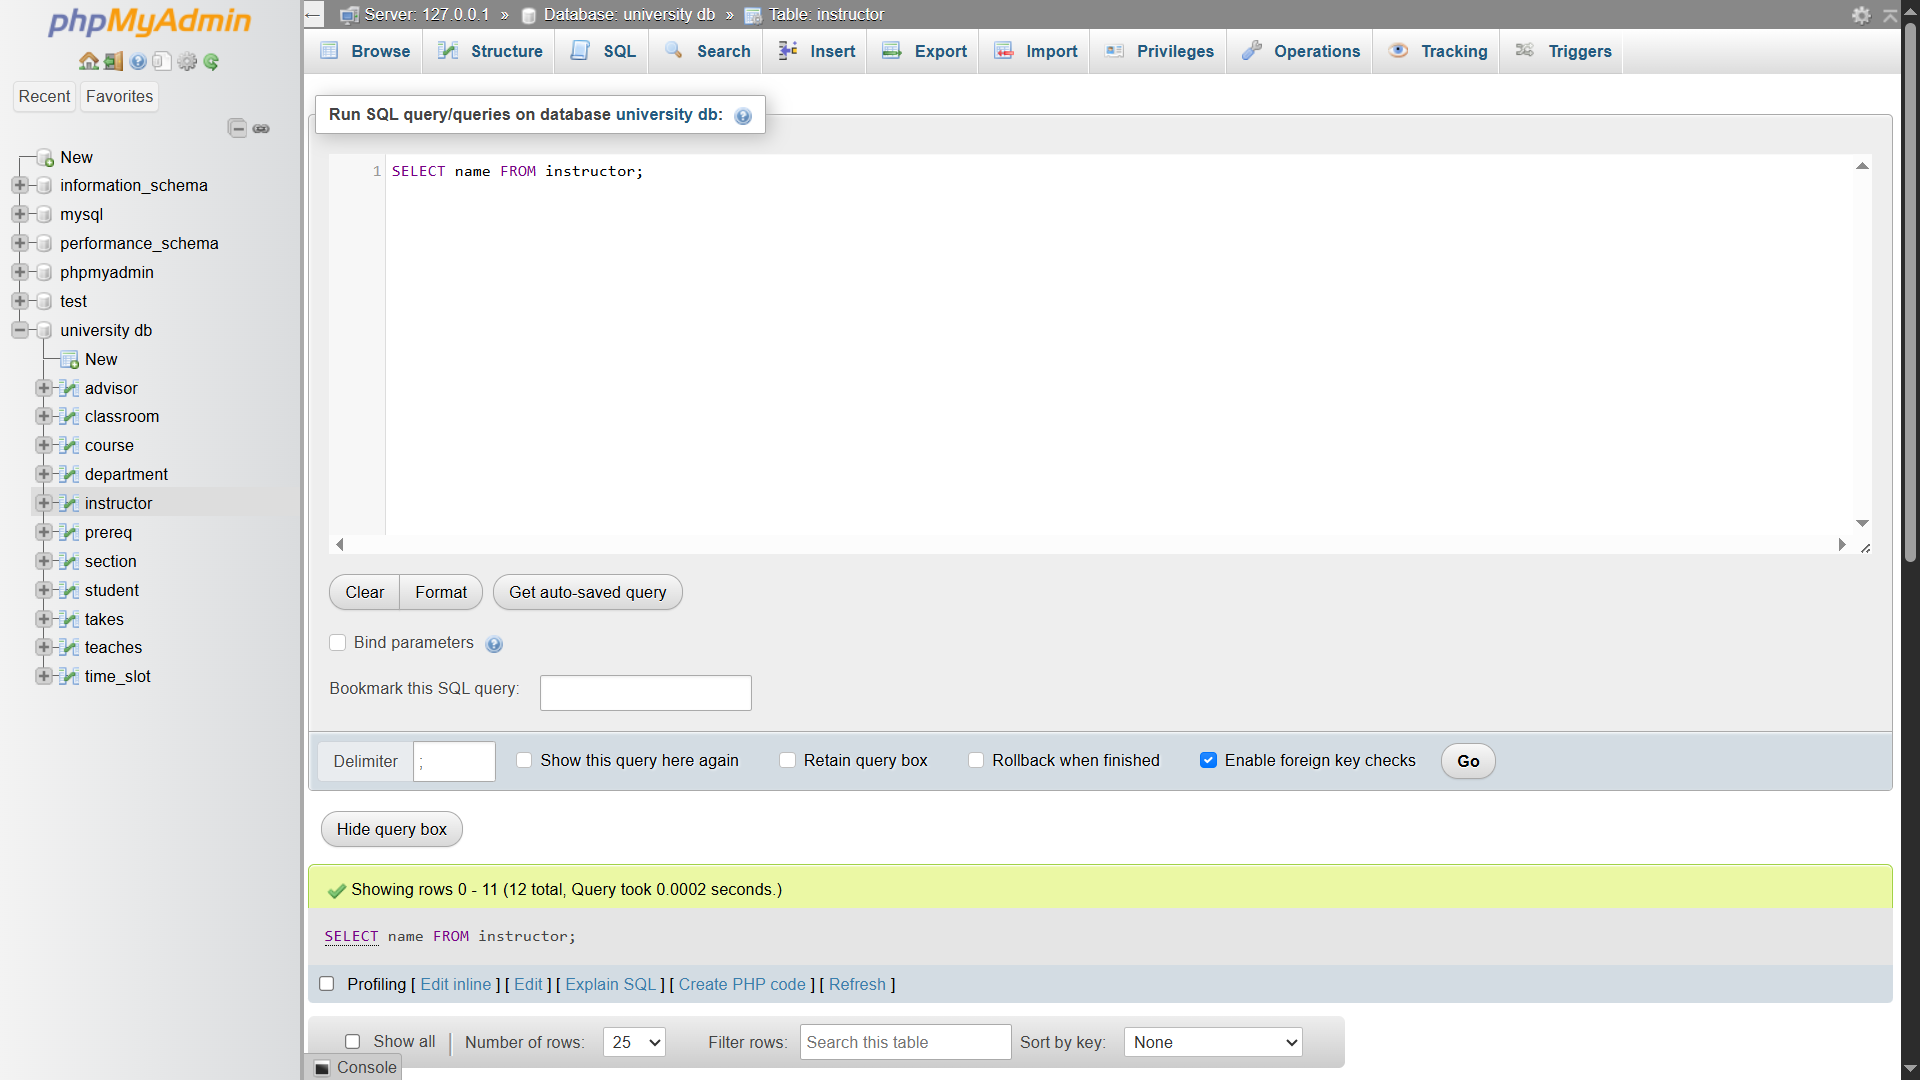
\includegraphics[width=1.0\textwidth]{fig/1.png}
\end{figure}

\begin{figure}[H]
    \centering
    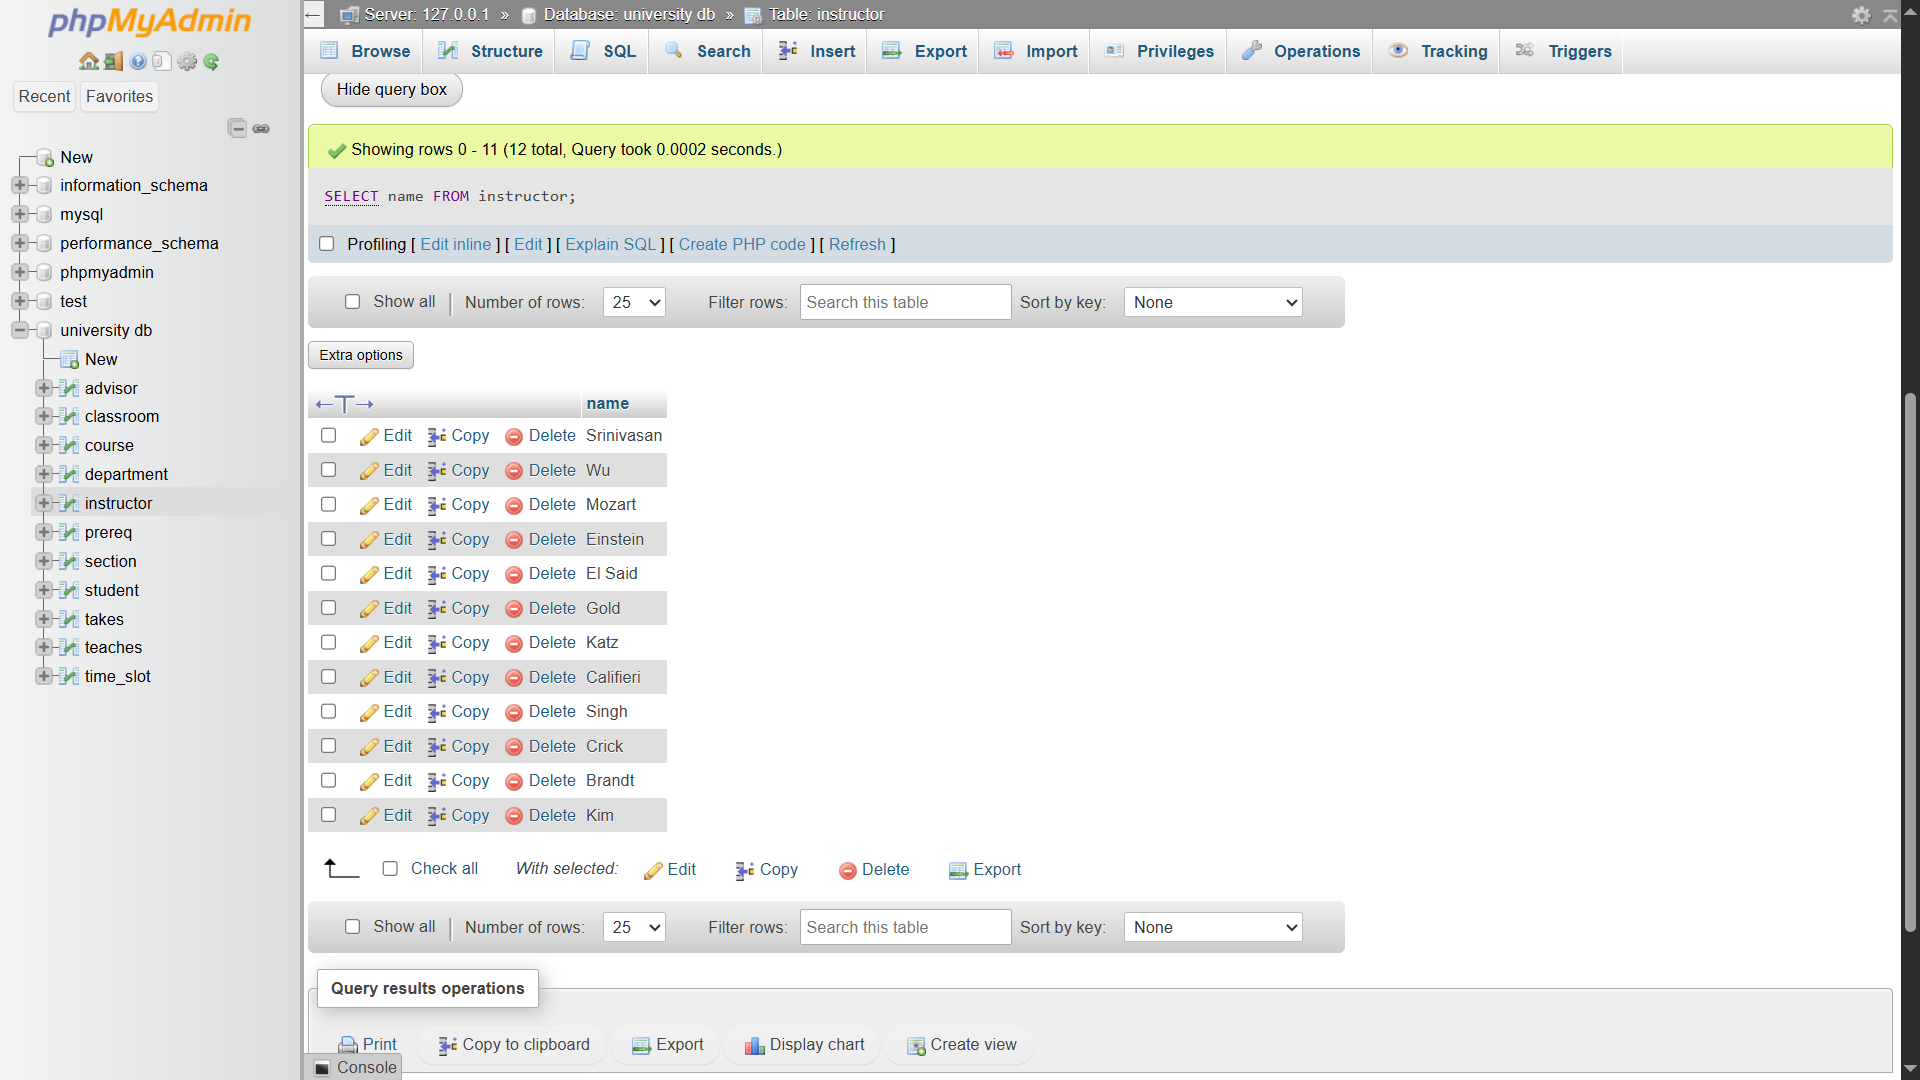
\includegraphics[width=1.0\textwidth]{fig/2.png}
\end{figure}

\begin{verbatim}
SELECT dept_name FROM instructor;
\end{verbatim}
\begin{figure}[H]
    \centering
    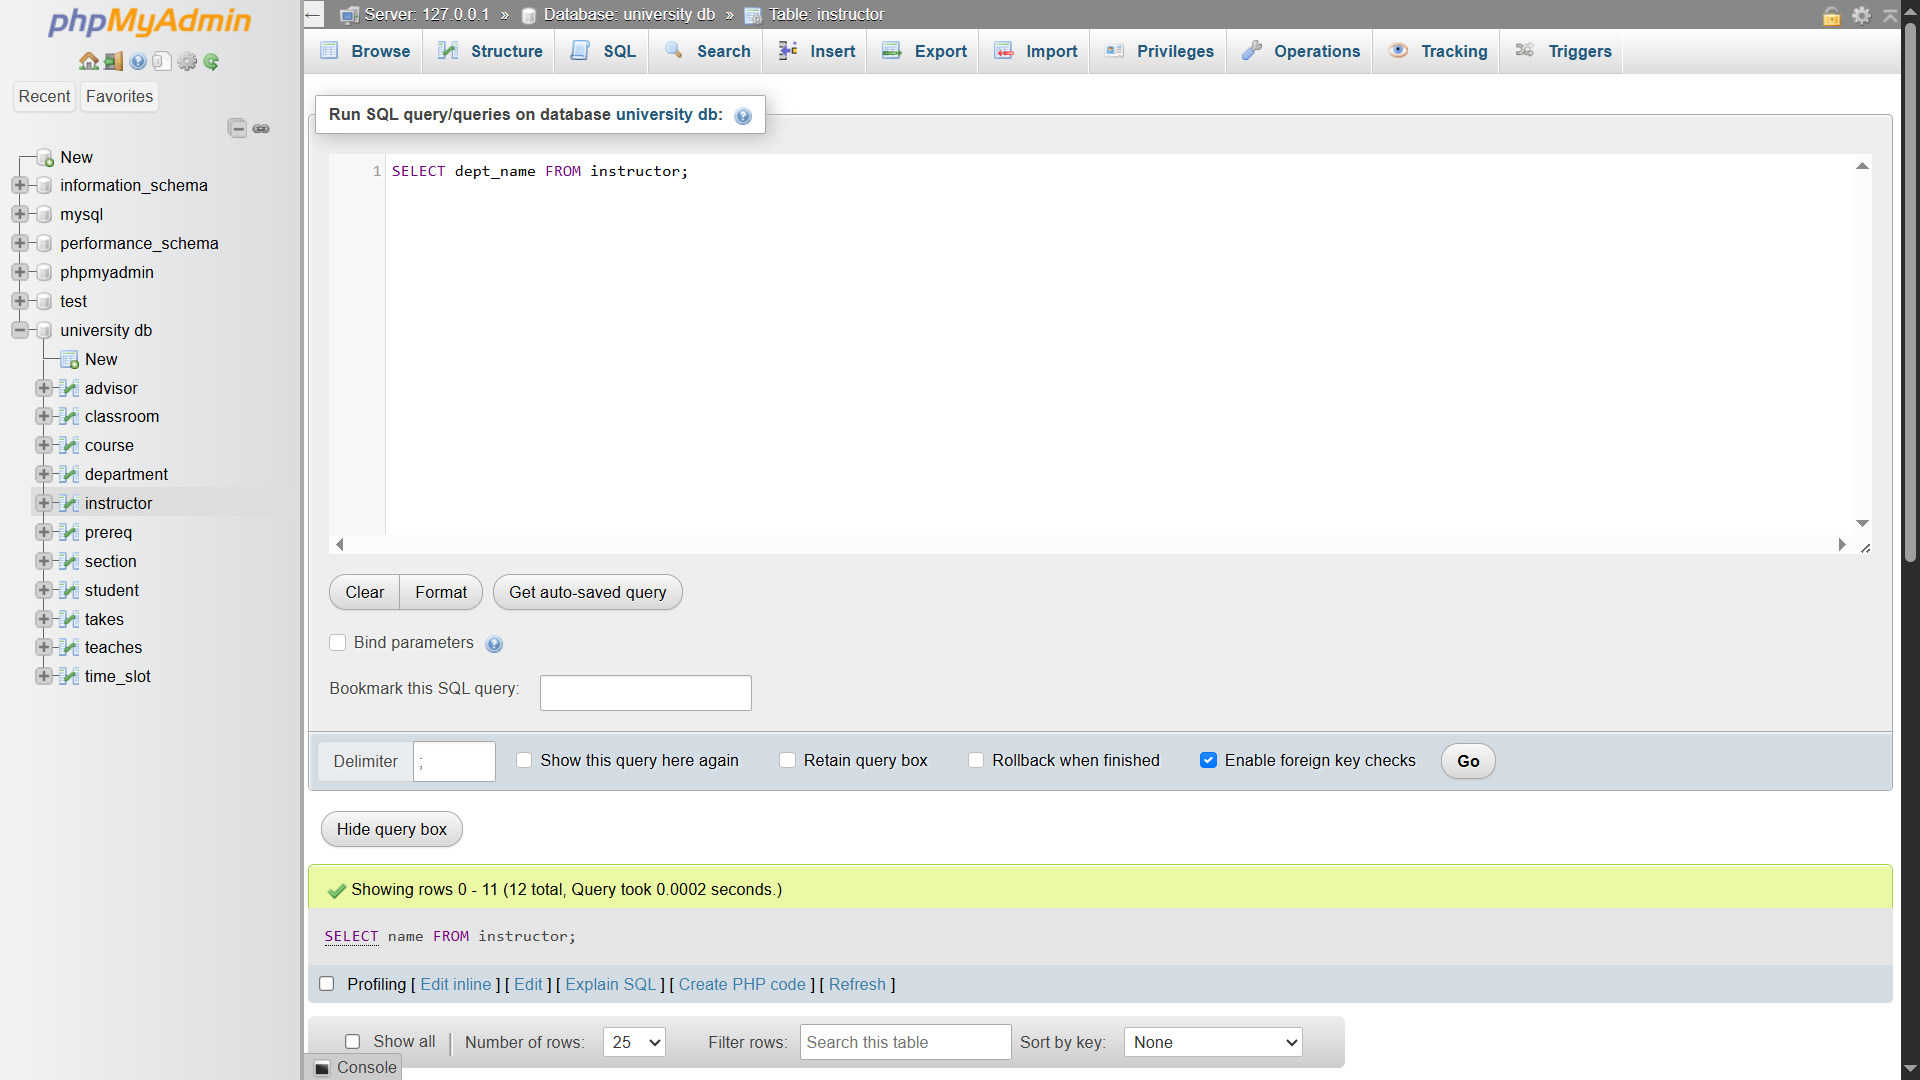
\includegraphics[width=1.0\textwidth]{fig/3.png}
\end{figure}

\begin{figure}[H]
    \centering
    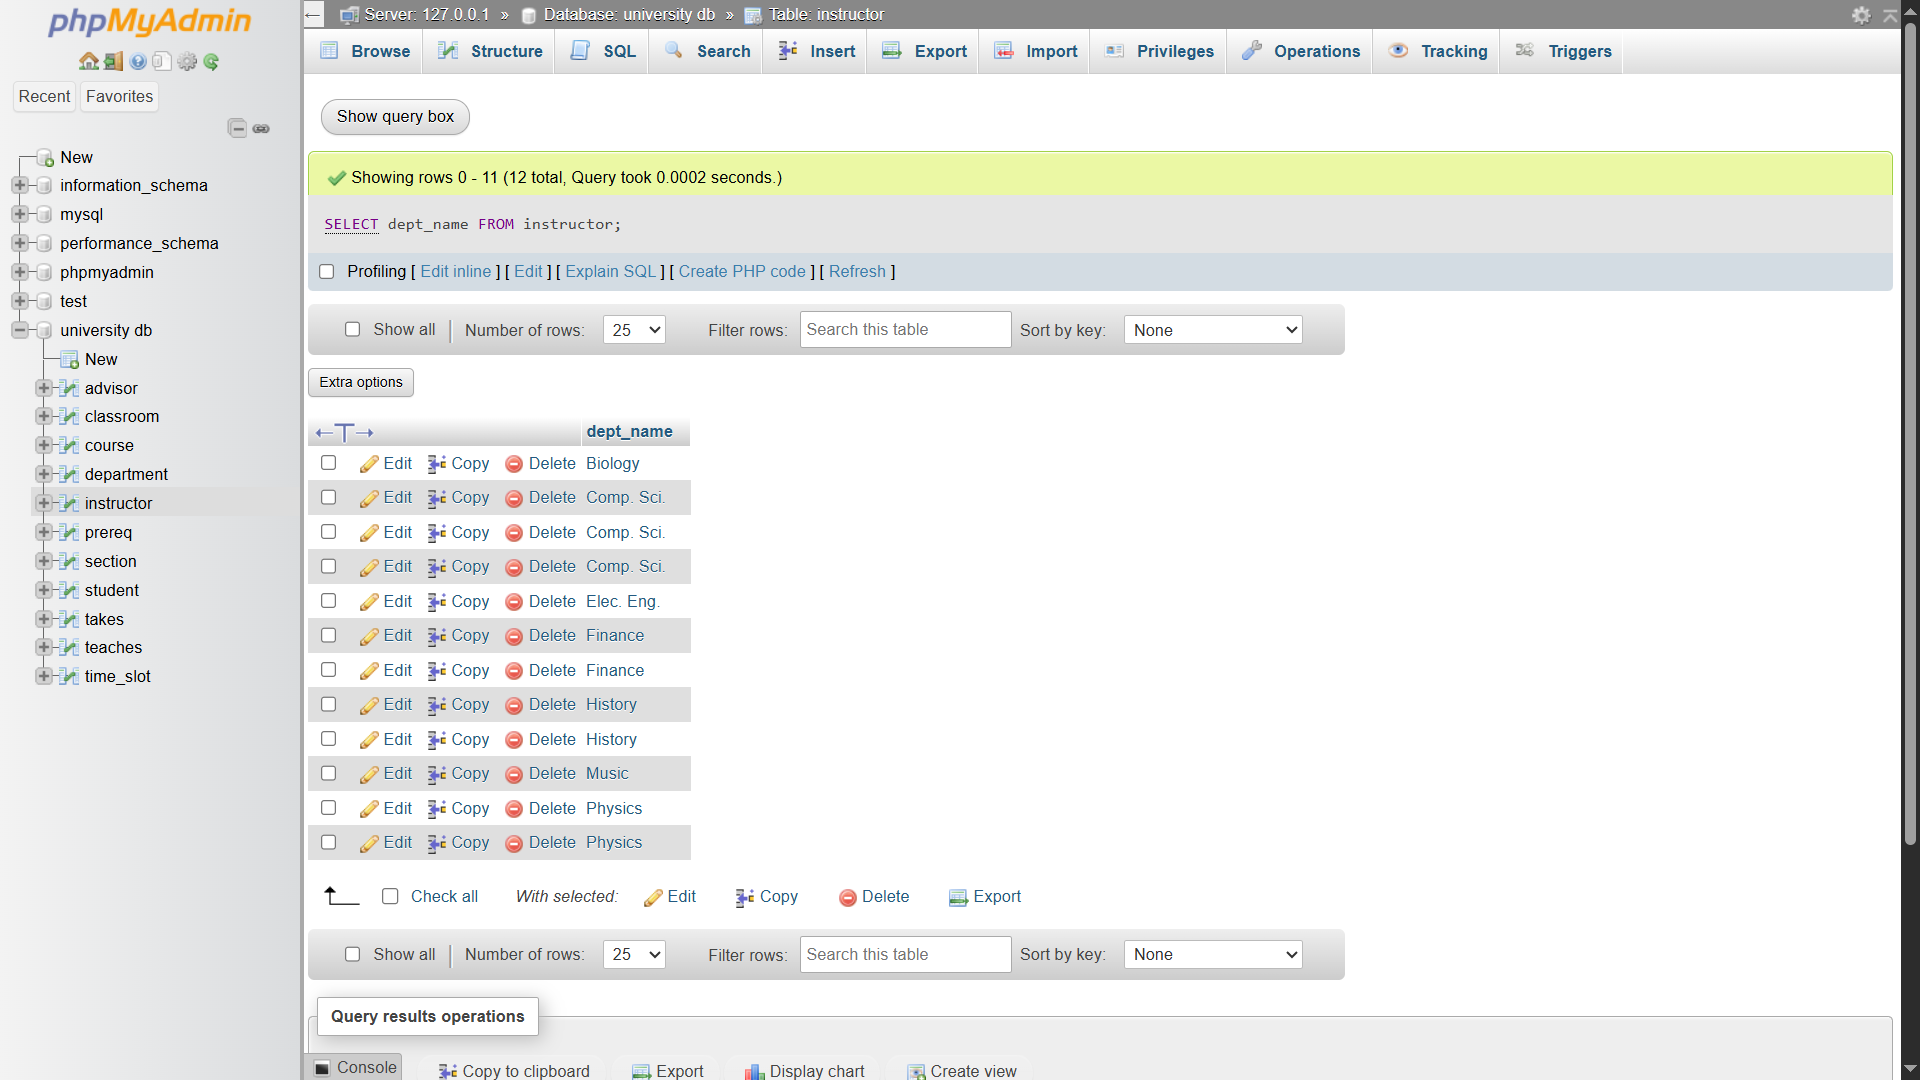
\includegraphics[width=1.0\textwidth]{fig/4.png}
\end{figure}

\begin{verbatim}
SELECT DISTINCT dept_name FROM instructor;
\end{verbatim}
\begin{figure}[H]
    \centering
    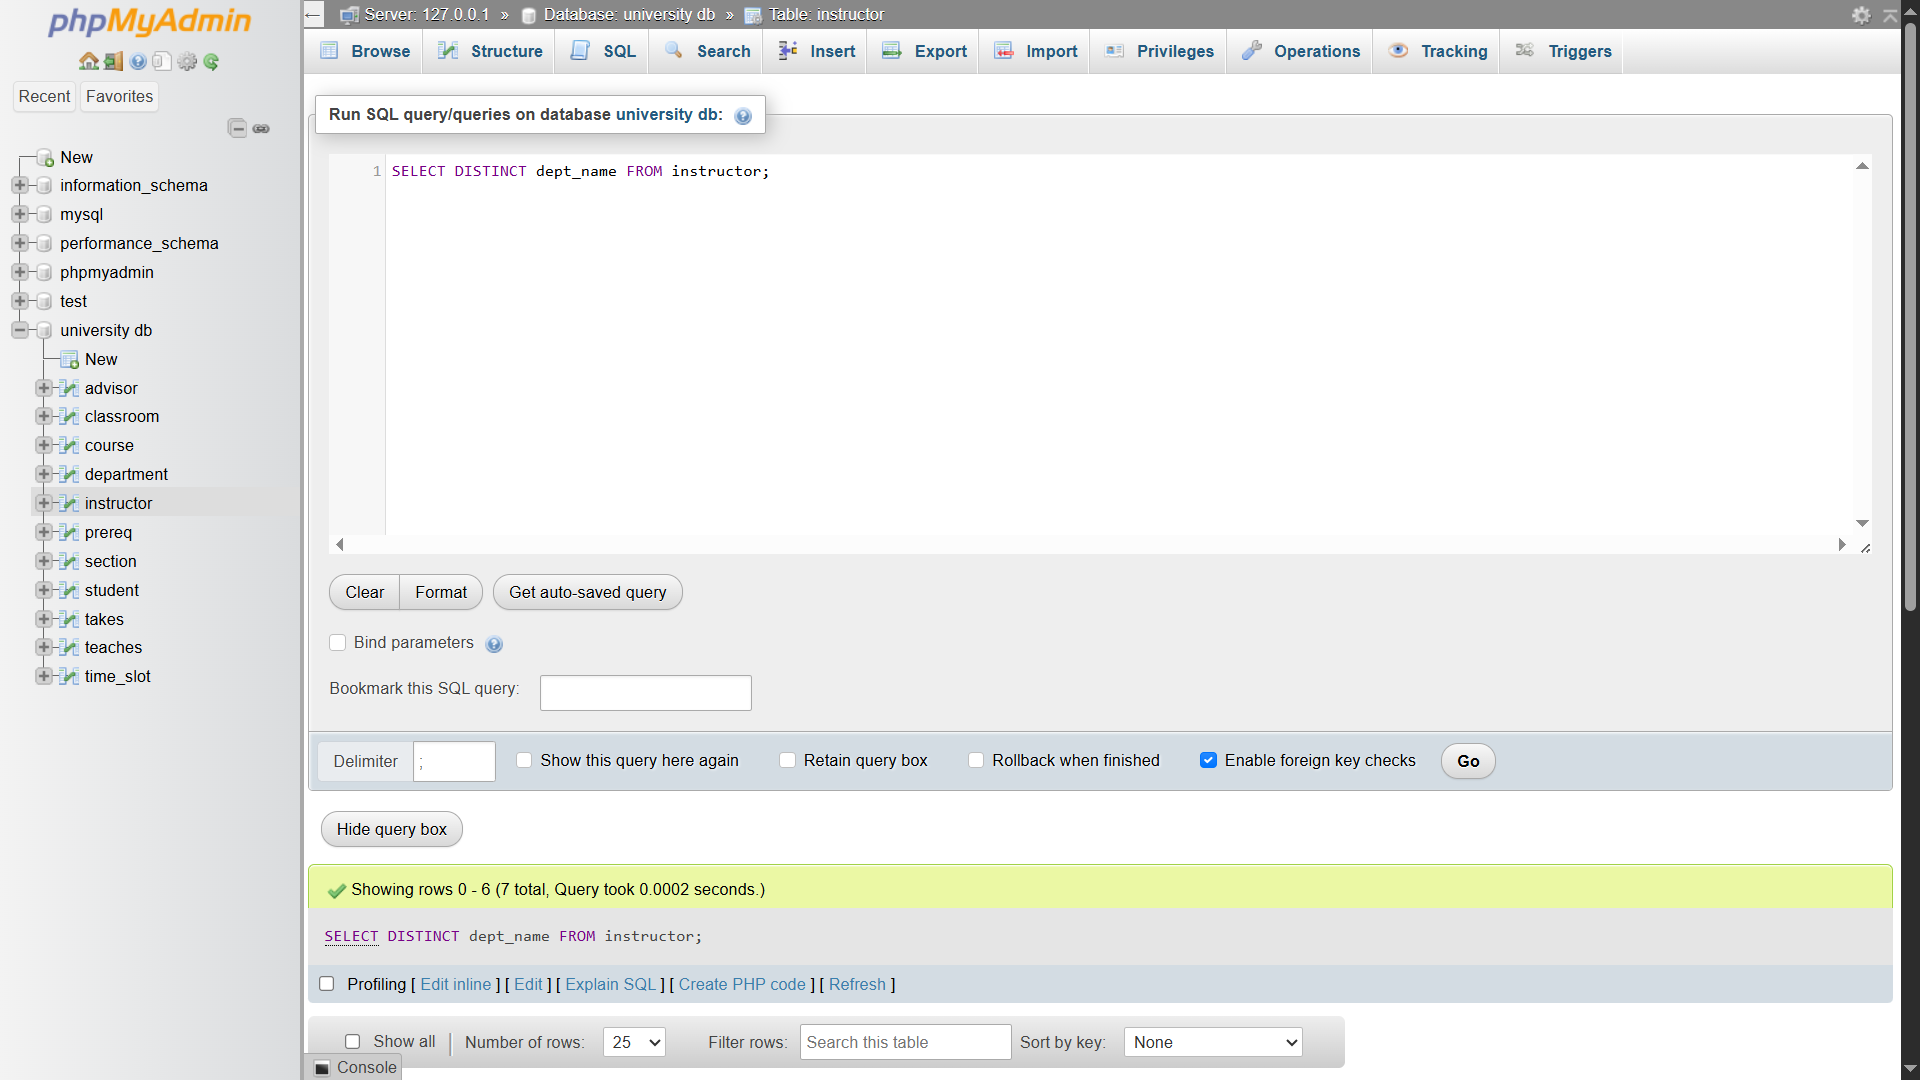
\includegraphics[width=1.0\textwidth]{fig/5.png}
\end{figure}

\begin{figure}[H]
    \centering
    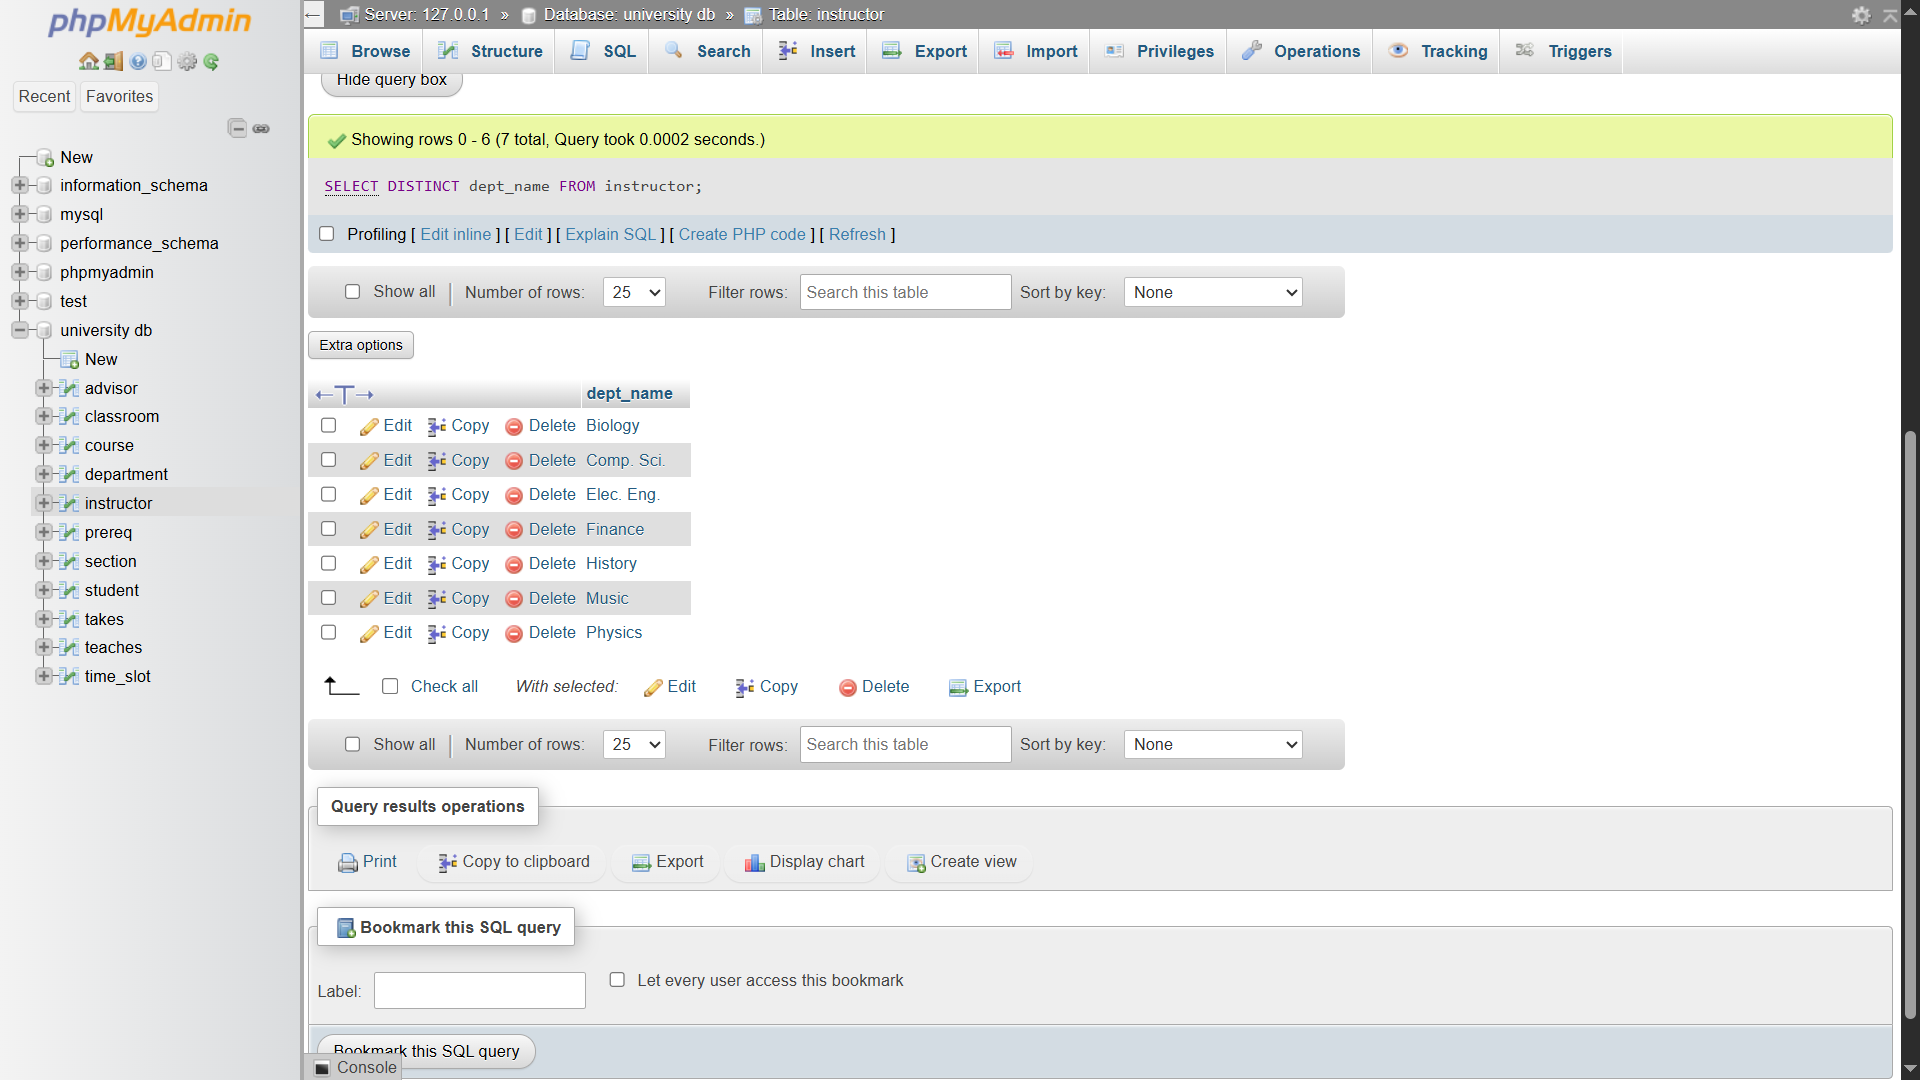
\includegraphics[width=1.0\textwidth]{fig/6.png}
\end{figure}

\begin{verbatim}
SELECT ALL dept_name FROM instructor;
\end{verbatim}
\begin{figure}[H]
    \centering
    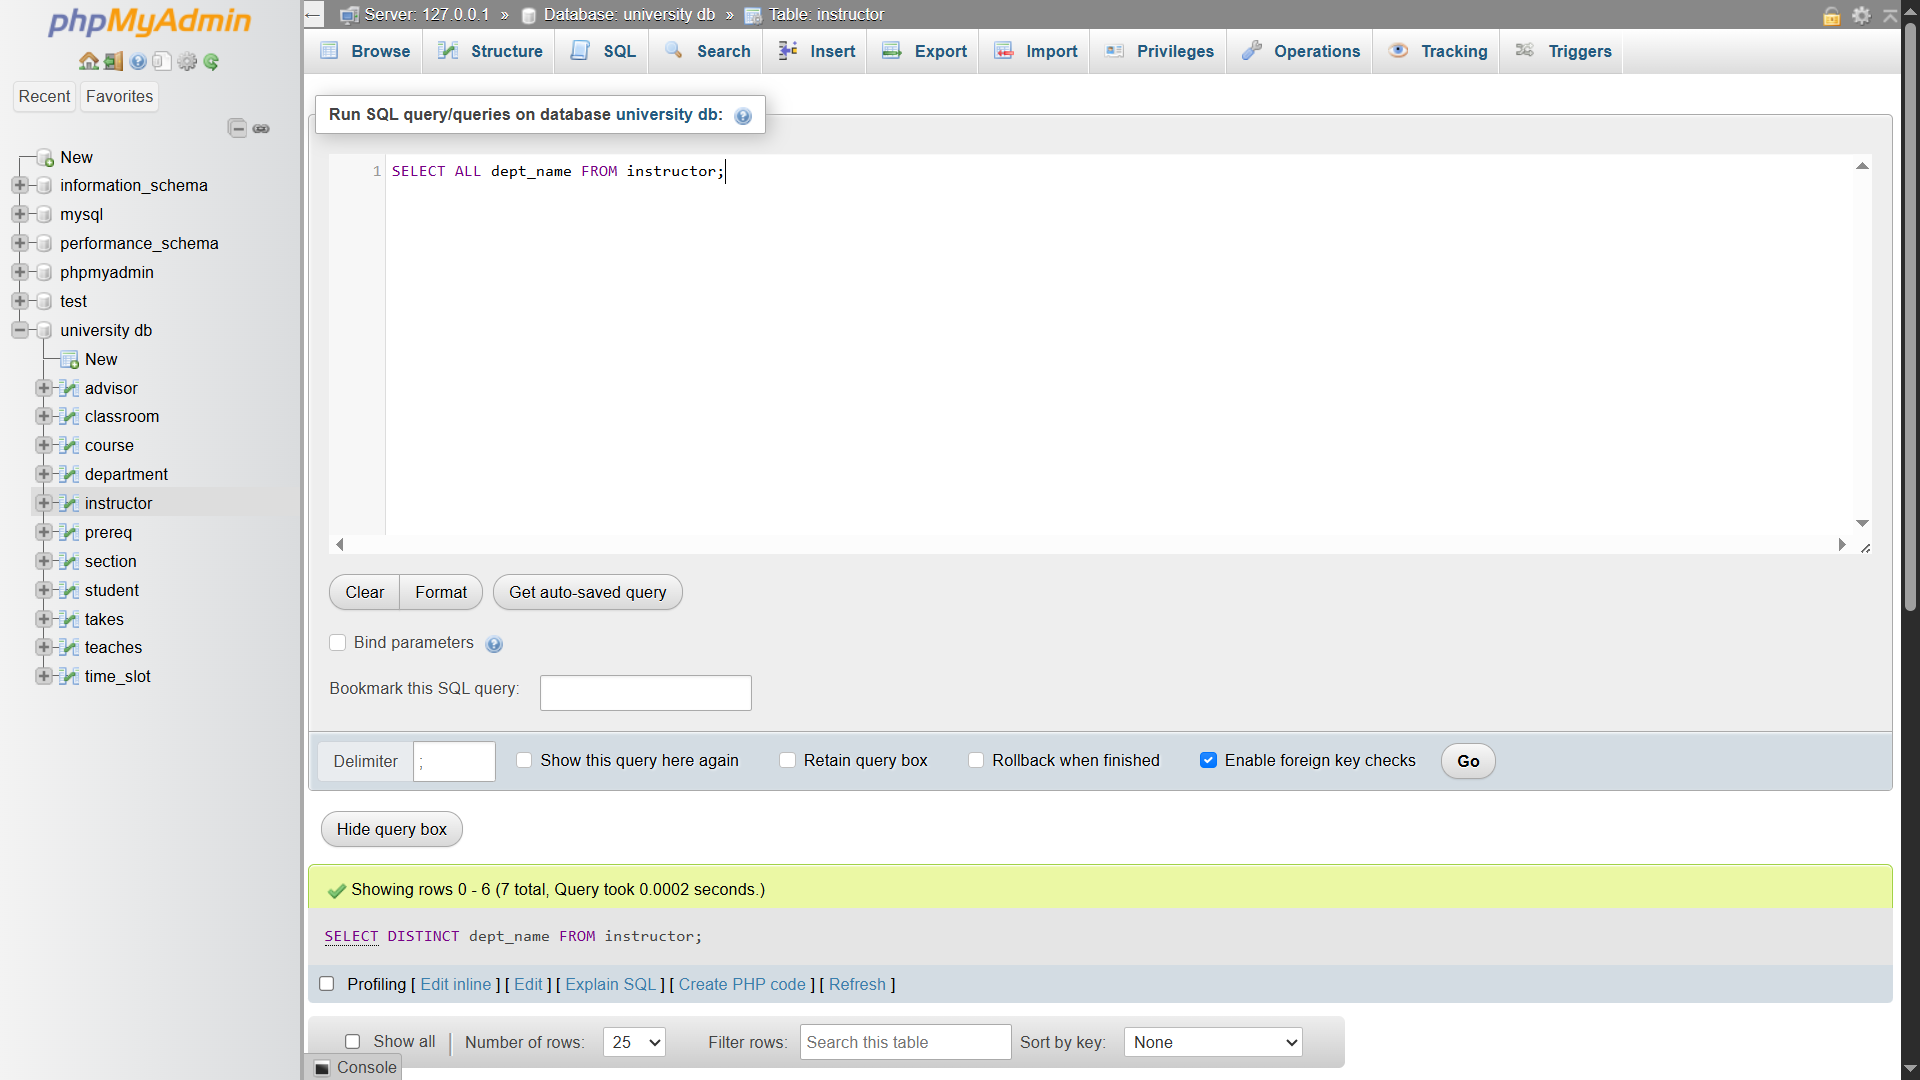
\includegraphics[width=1.0\textwidth]{fig/7.png}
\end{figure}

\begin{figure}[H]
    \centering
    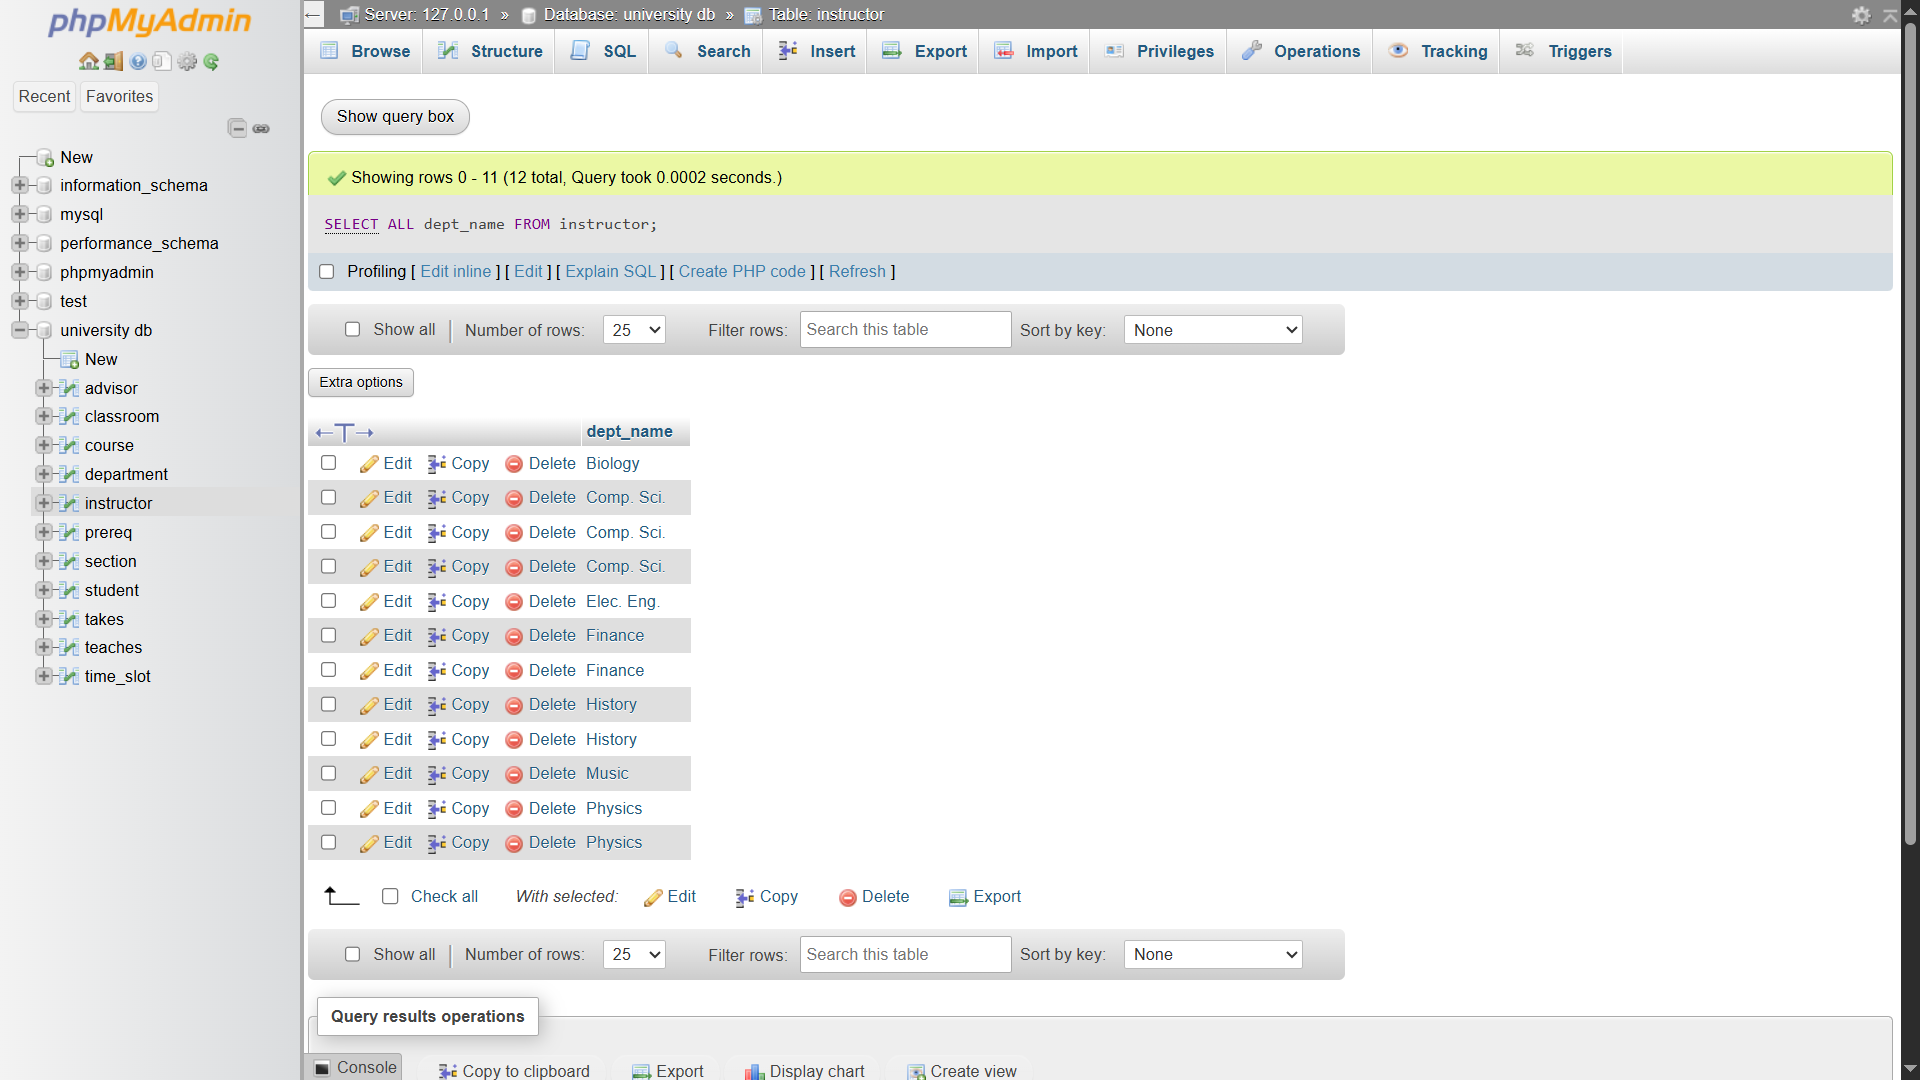
\includegraphics[width=1.0\textwidth]{fig/8.png}
\end{figure}

\begin{verbatim}
SELECT ID, name, salary * 5 FROM instructor;
\end{verbatim}
\begin{figure}[H]
    \centering
    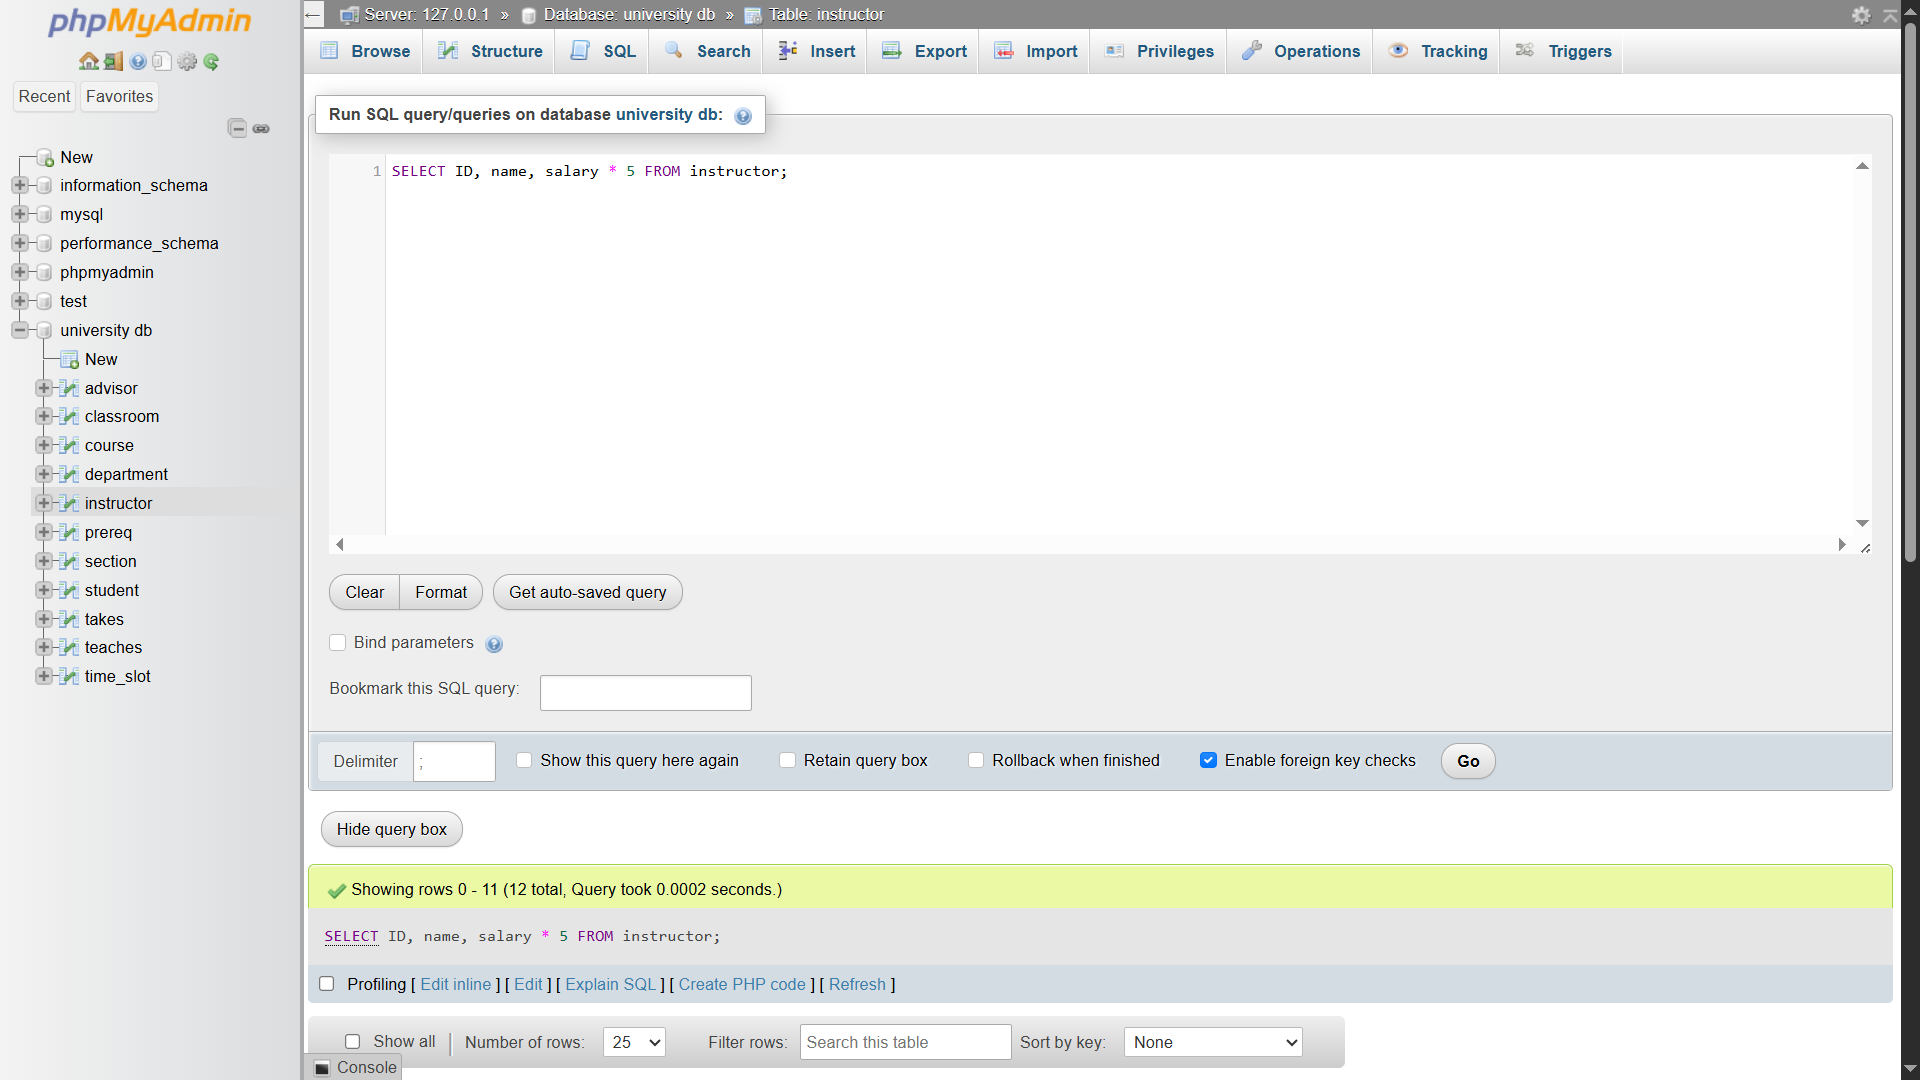
\includegraphics[width=1.0\textwidth]{fig/9.png}
\end{figure}

\begin{figure}[H]
    \centering
    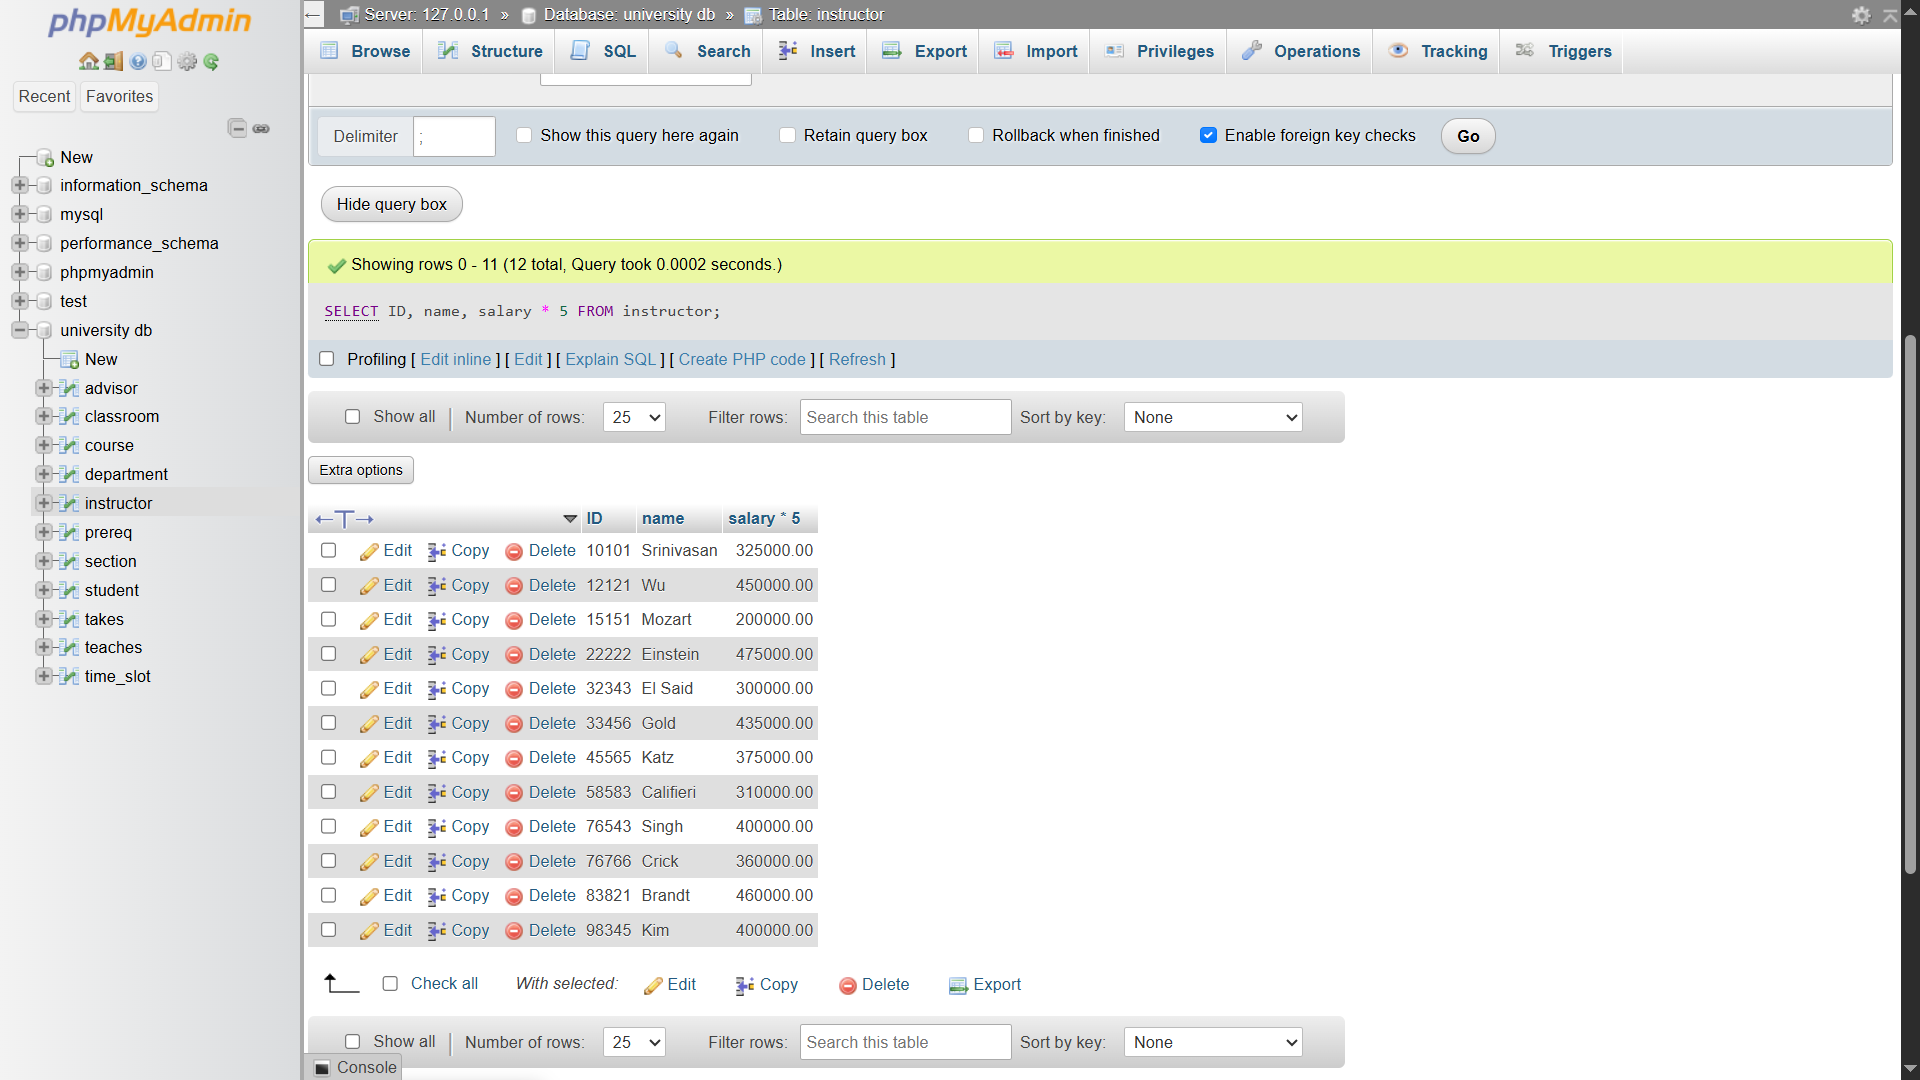
\includegraphics[width=1.0\textwidth]{fig/10.png}
\end{figure}

\begin{verbatim}
SELECT ID, name, salary * 5 AS monthly_salary FROM instructor;
\end{verbatim}
\begin{figure}[H]
    \centering
    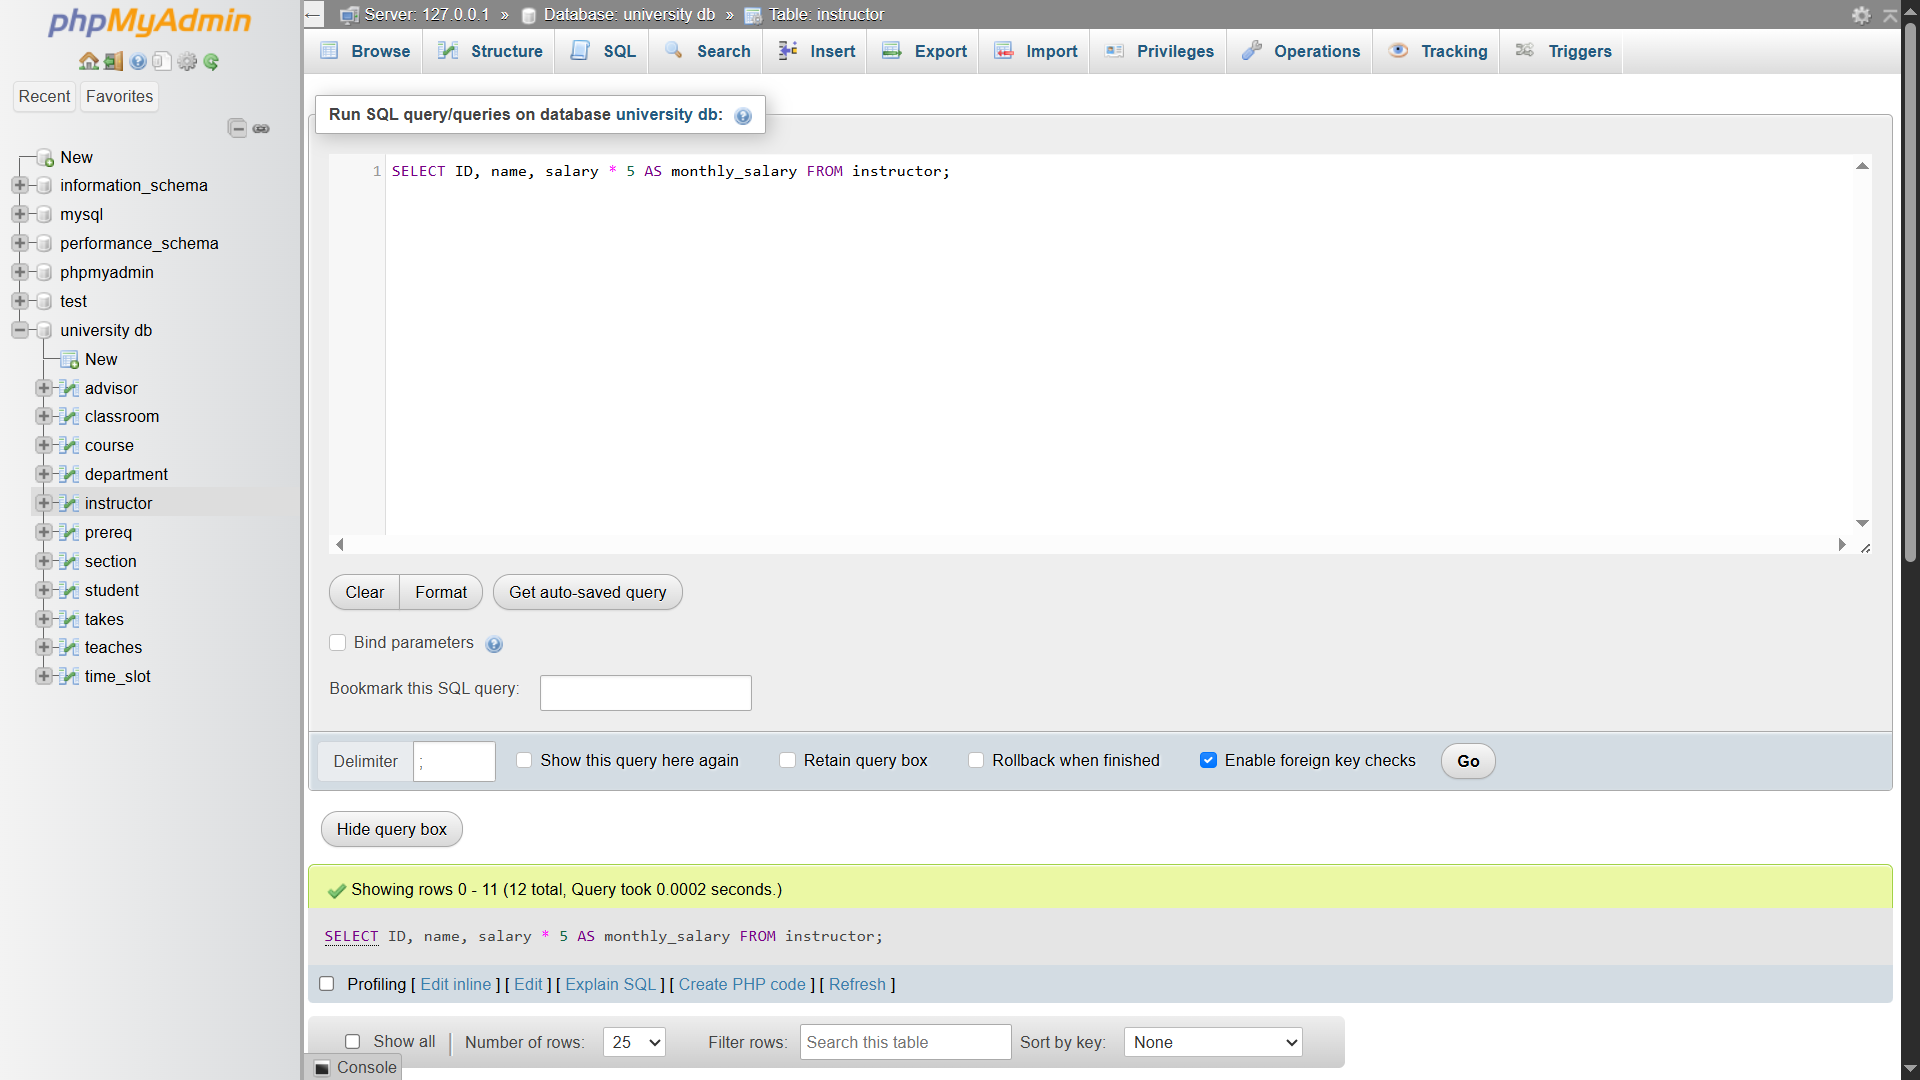
\includegraphics[width=1.0\textwidth]{fig/11.png}
\end{figure}

\begin{figure}[H]
    \centering
    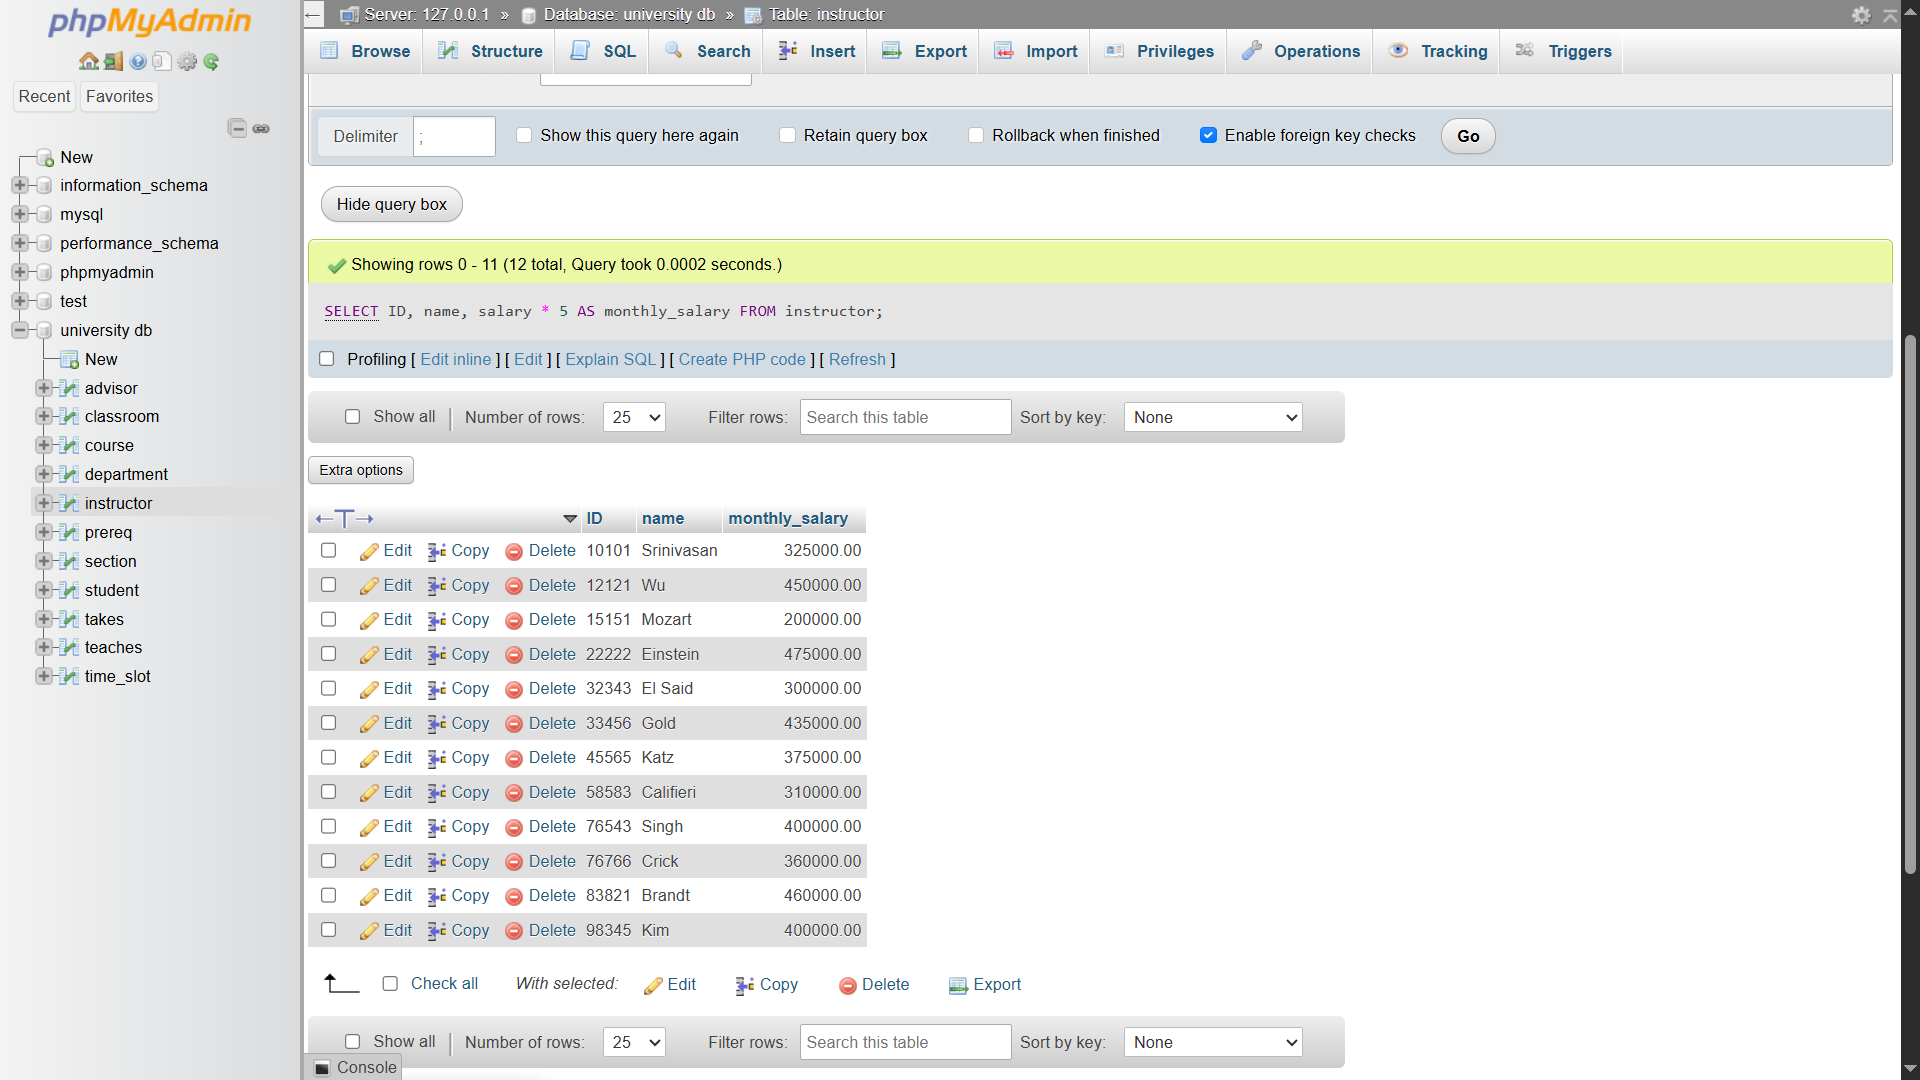
\includegraphics[width=1.0\textwidth]{fig/12.png}
\end{figure}

\begin{verbatim}
SELECT name FROM instructor 
WHERE dept_name = 'Comp. Sci' AND salary > 70000;
\end{verbatim}
\begin{figure}[H]
    \centering
    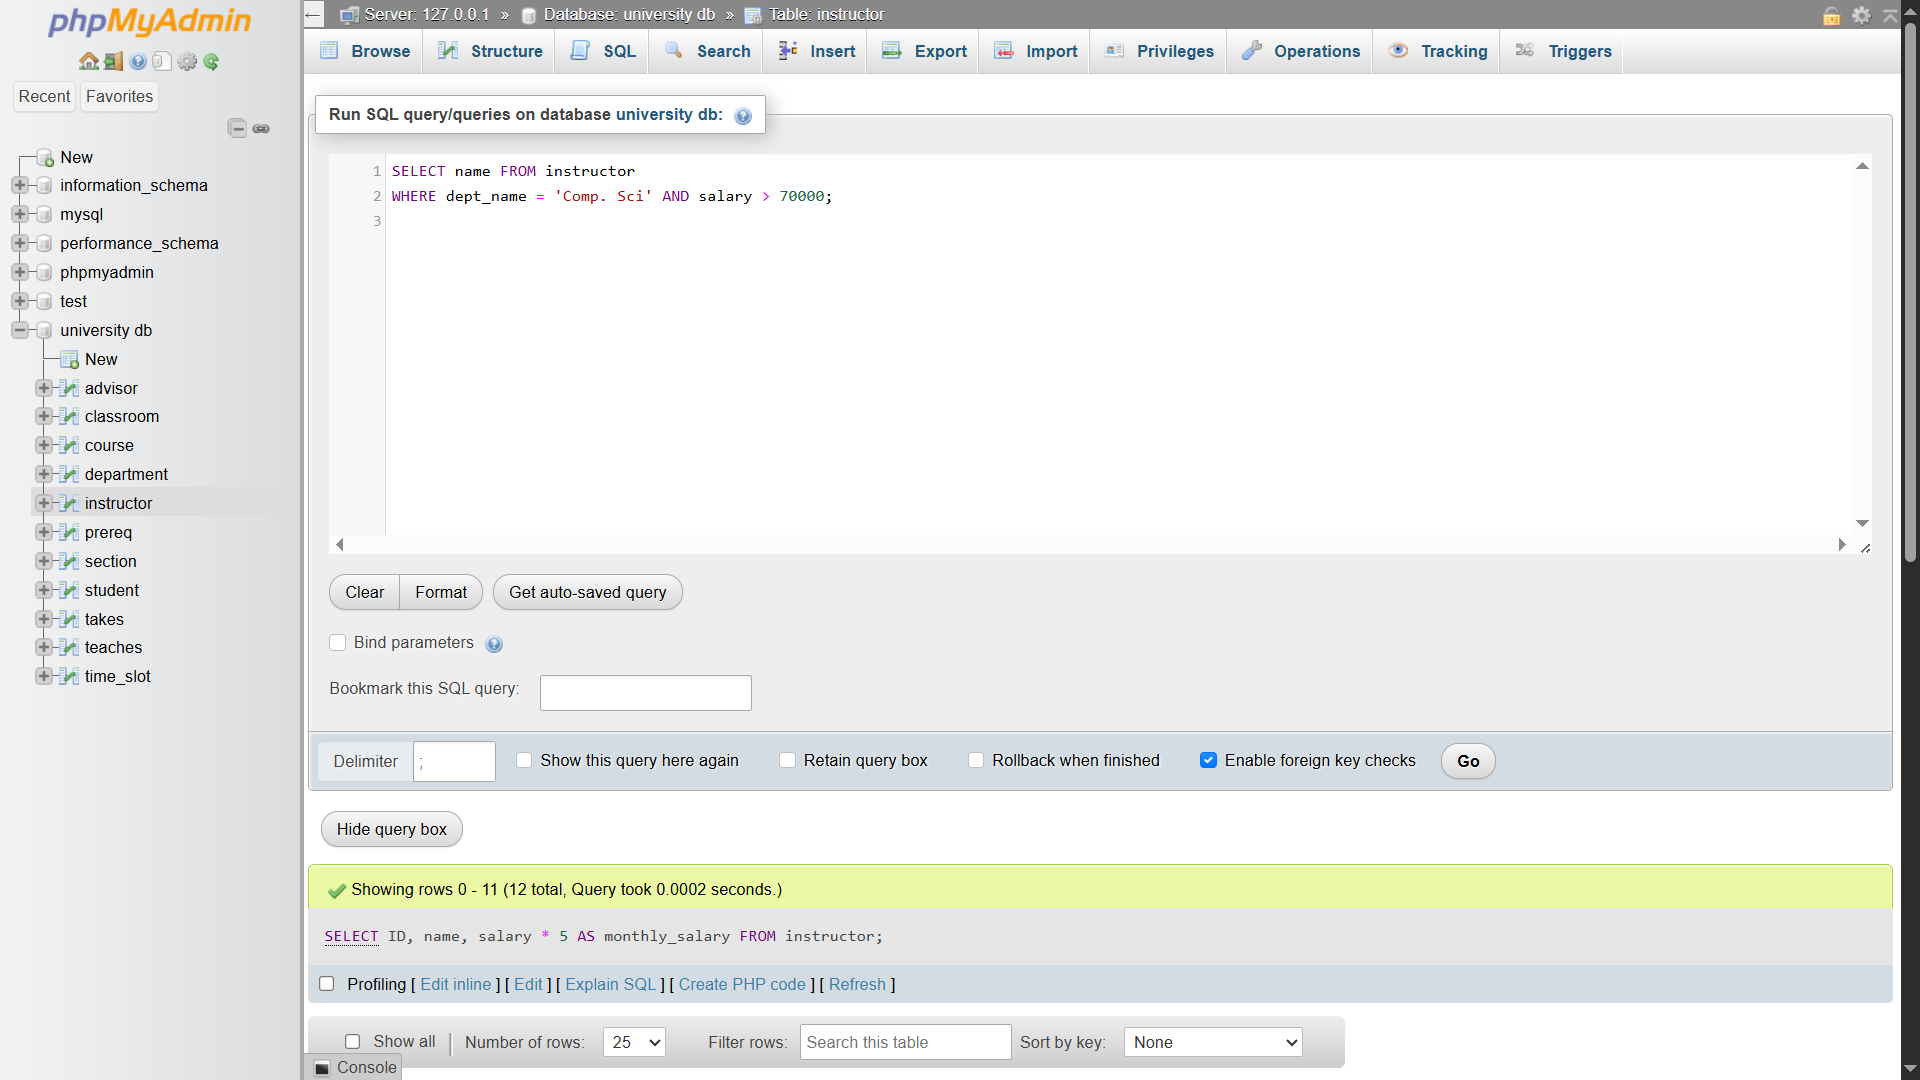
\includegraphics[width=1.0\textwidth]{fig/13.png}
\end{figure}

\begin{figure}[H]
    \centering
    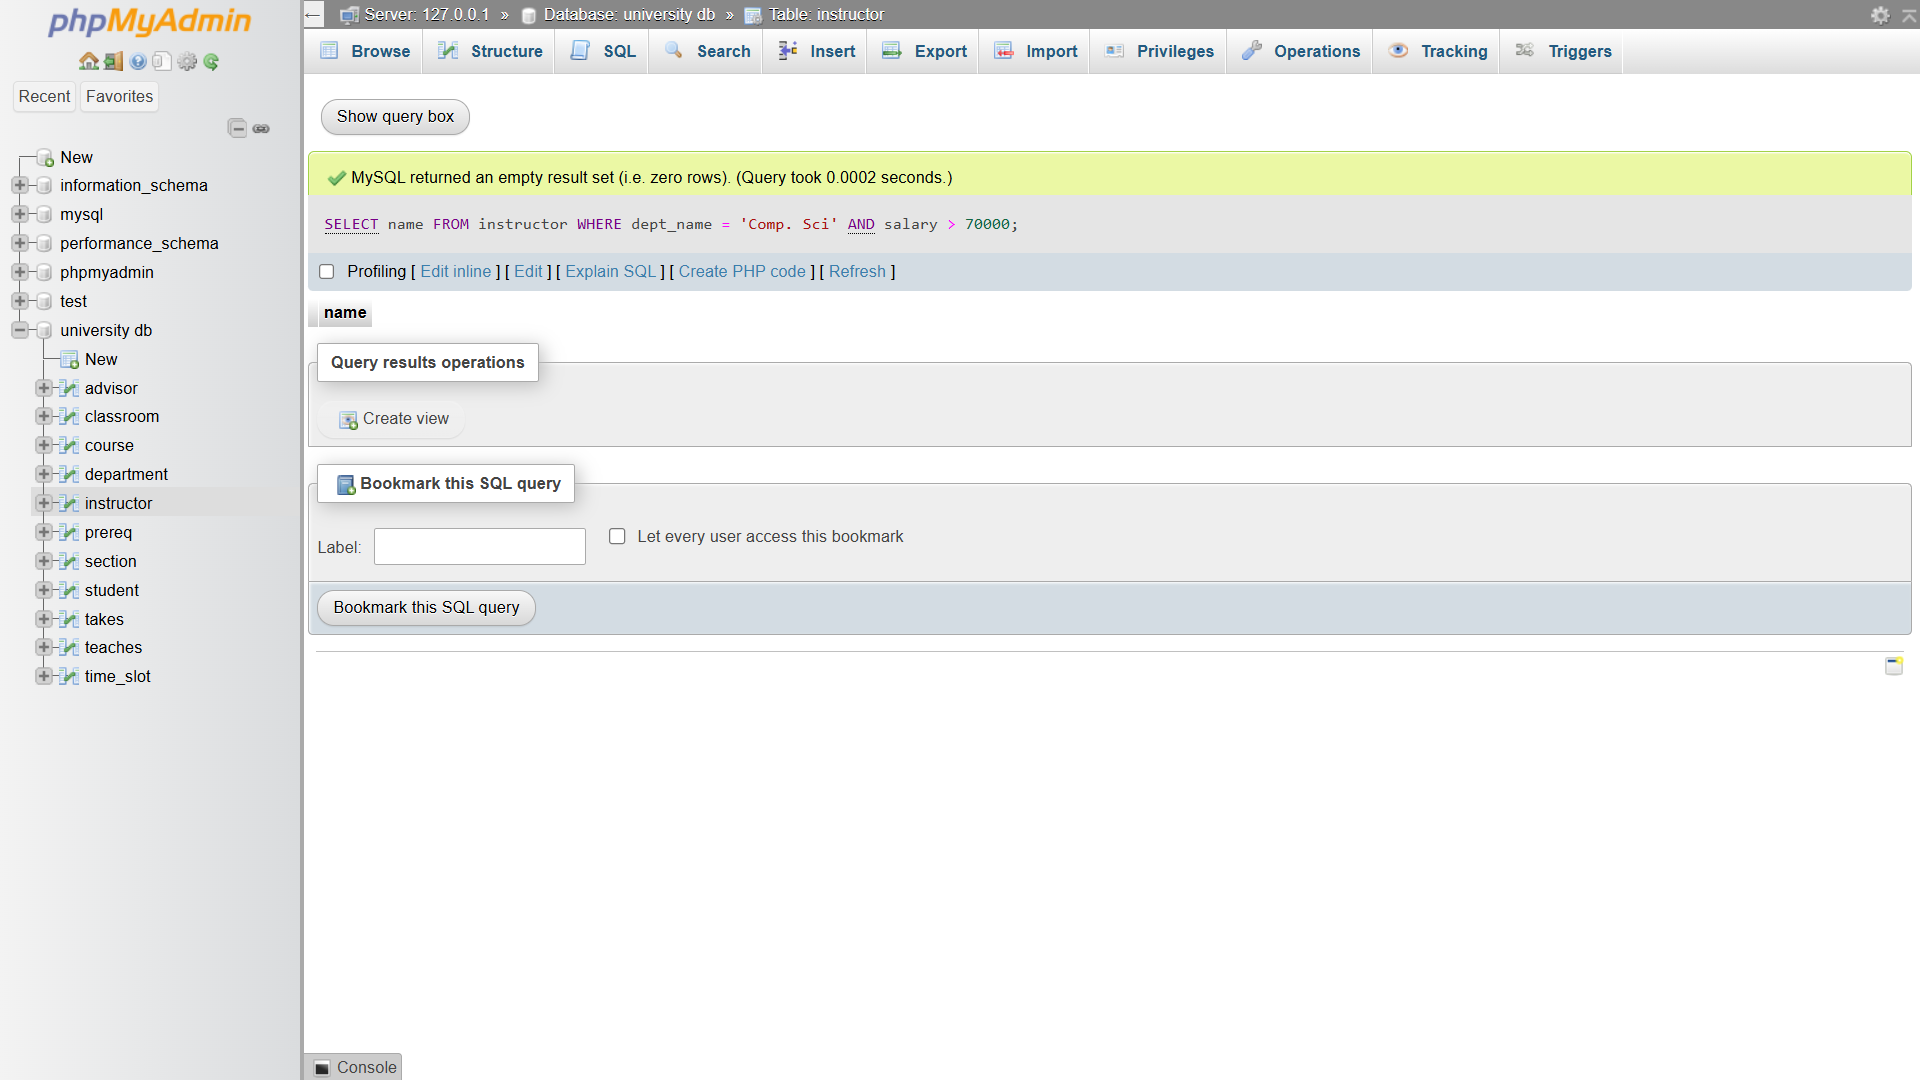
\includegraphics[width=1.0\textwidth]{fig/14.png}
\end{figure}

\begin{verbatim}
SELECT name, instructor.dept_name, building 
FROM instructor, department 
WHERE instructor.dept_name = department.dept_name;
\end{verbatim}
\begin{figure}[H]
    \centering
    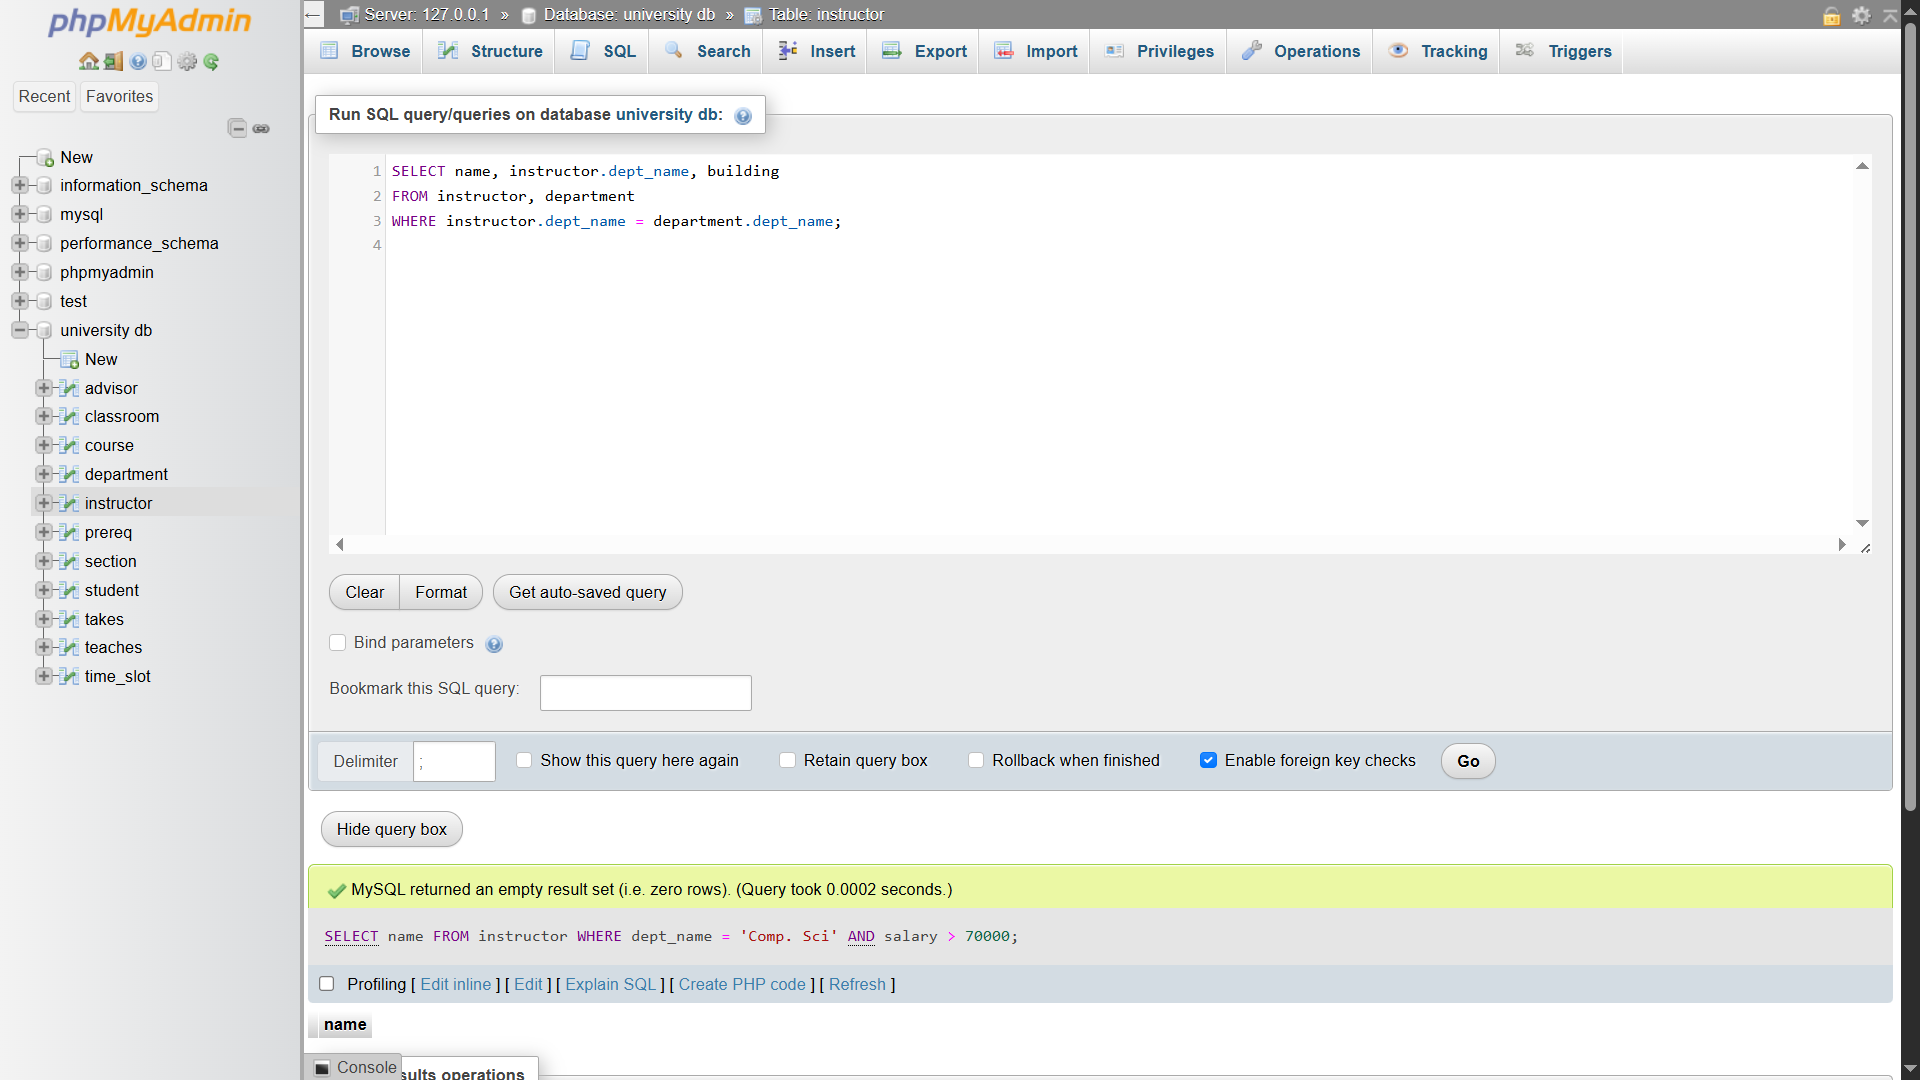
\includegraphics[width=1.0\textwidth]{fig/15.png}
\end{figure}

\begin{figure}[H]
    \centering
    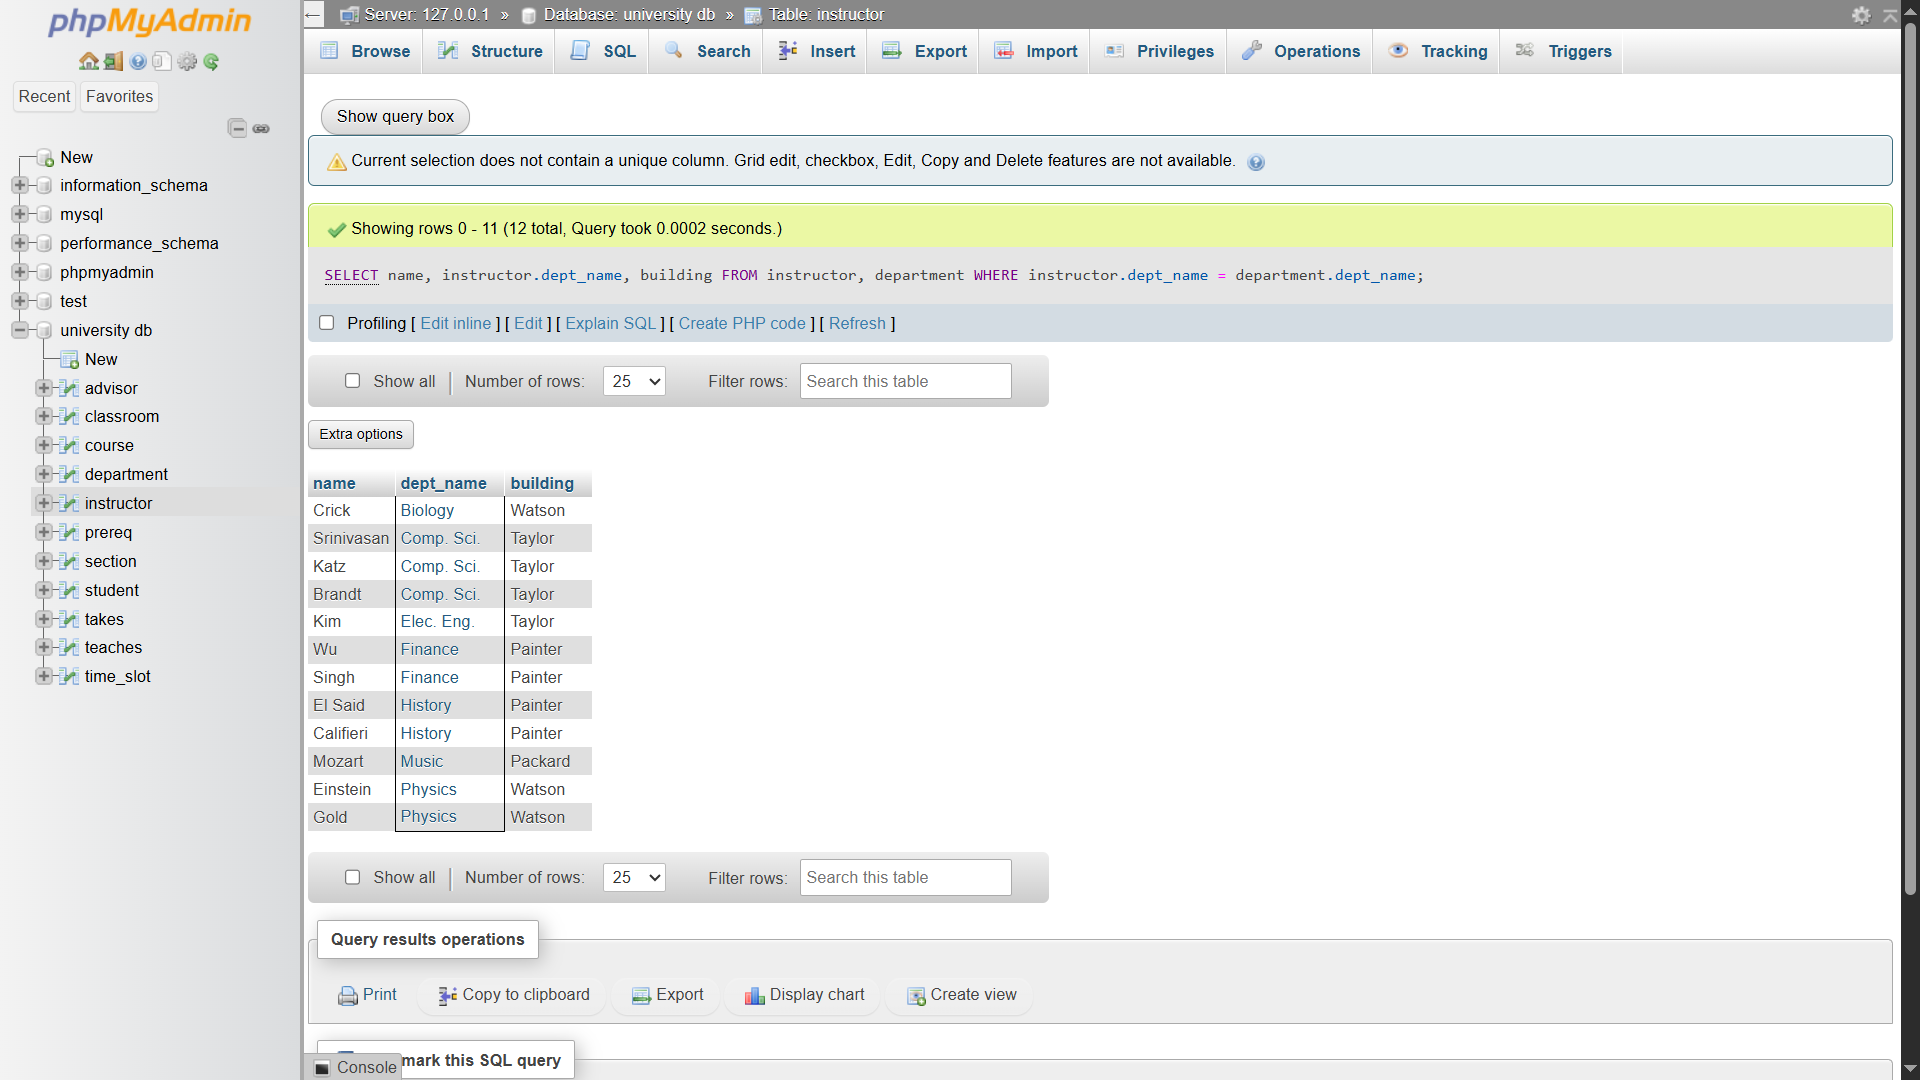
\includegraphics[width=1.0\textwidth]{fig/16.png}
\end{figure}

\begin{verbatim}
SELECT * FROM instructor, teaches;
\end{verbatim}
\begin{figure}[H]
    \centering
    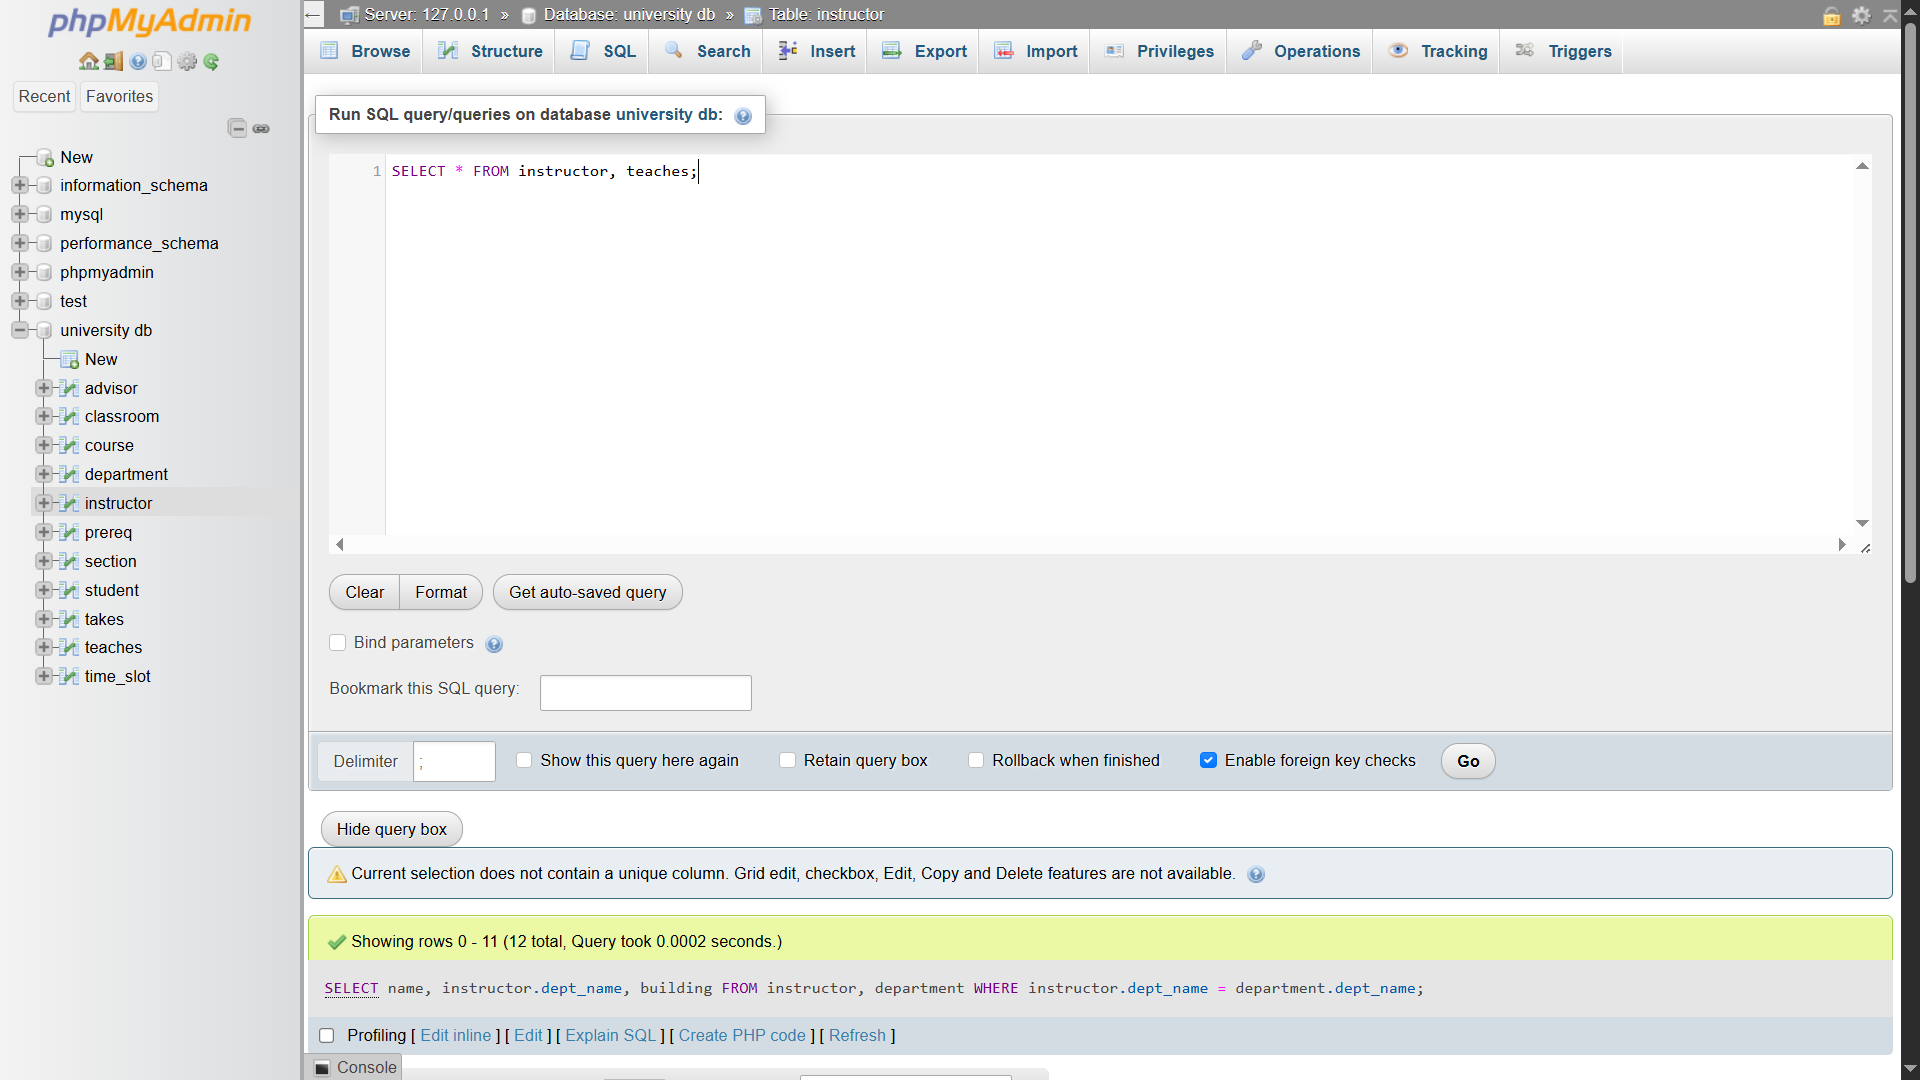
\includegraphics[width=1.0\textwidth]{fig/17.png}
\end{figure}

\begin{figure}[H]
    \centering
    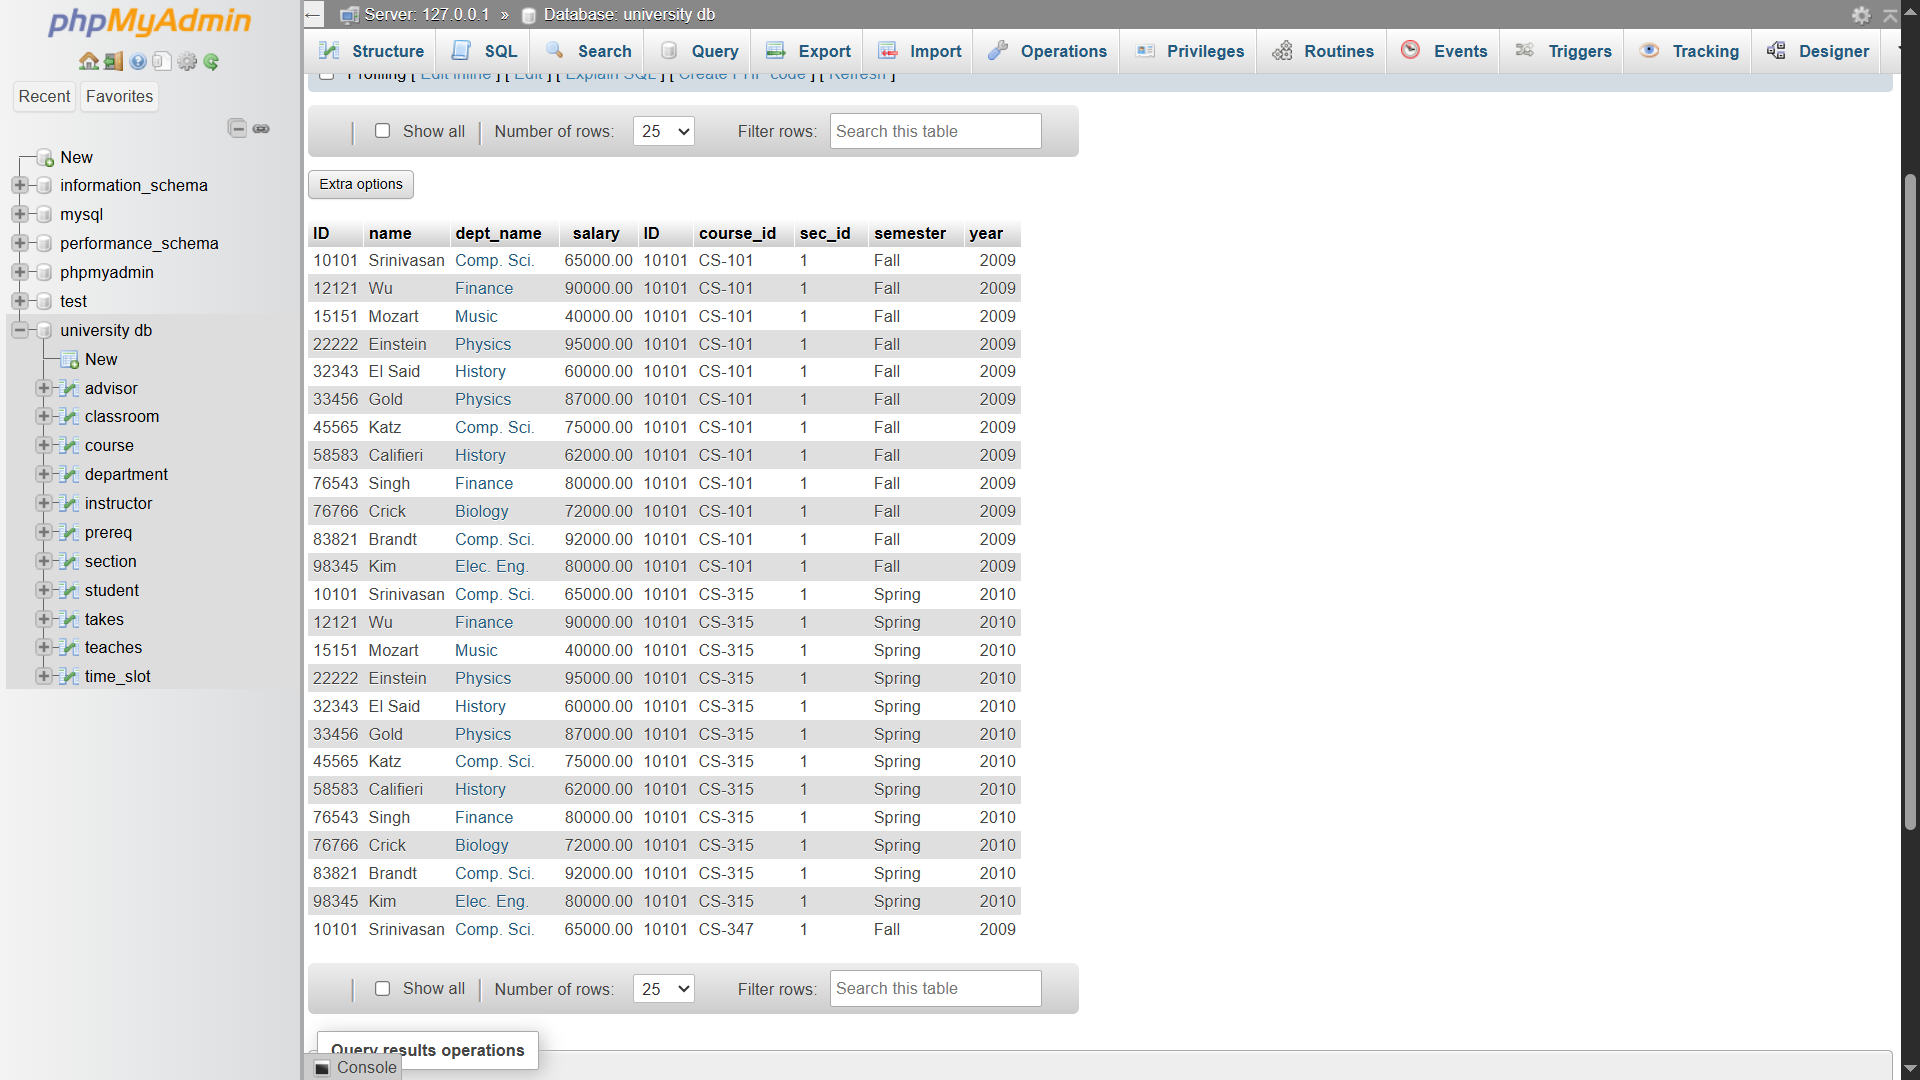
\includegraphics[width=1.0\textwidth]{fig/18.png}
\end{figure}

\begin{verbatim}
SELECT name, course_id 
FROM instructor, teaches 
WHERE instructor.ID = teaches.ID;
\end{verbatim}
\begin{figure}[H]
    \centering
    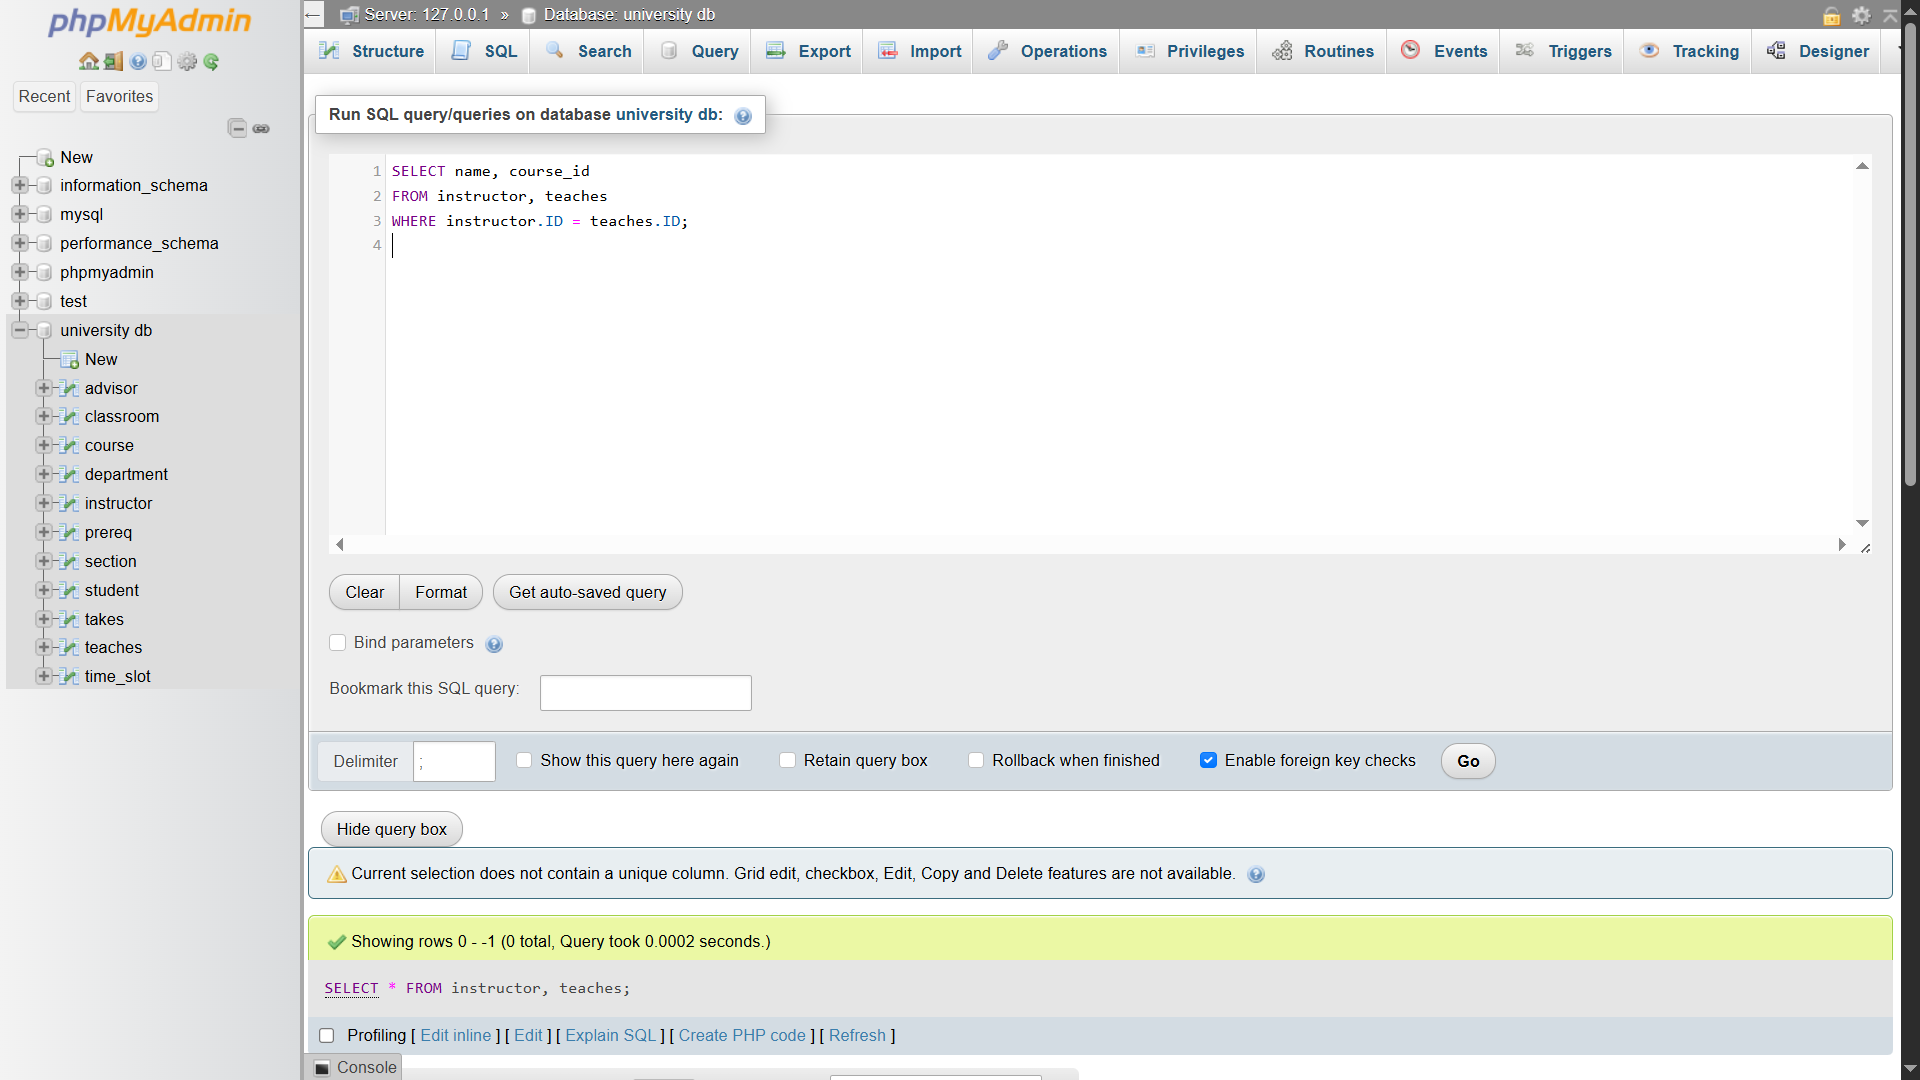
\includegraphics[width=1.0\textwidth]{fig/19.png}
\end{figure}

\begin{figure}[H]
    \centering
    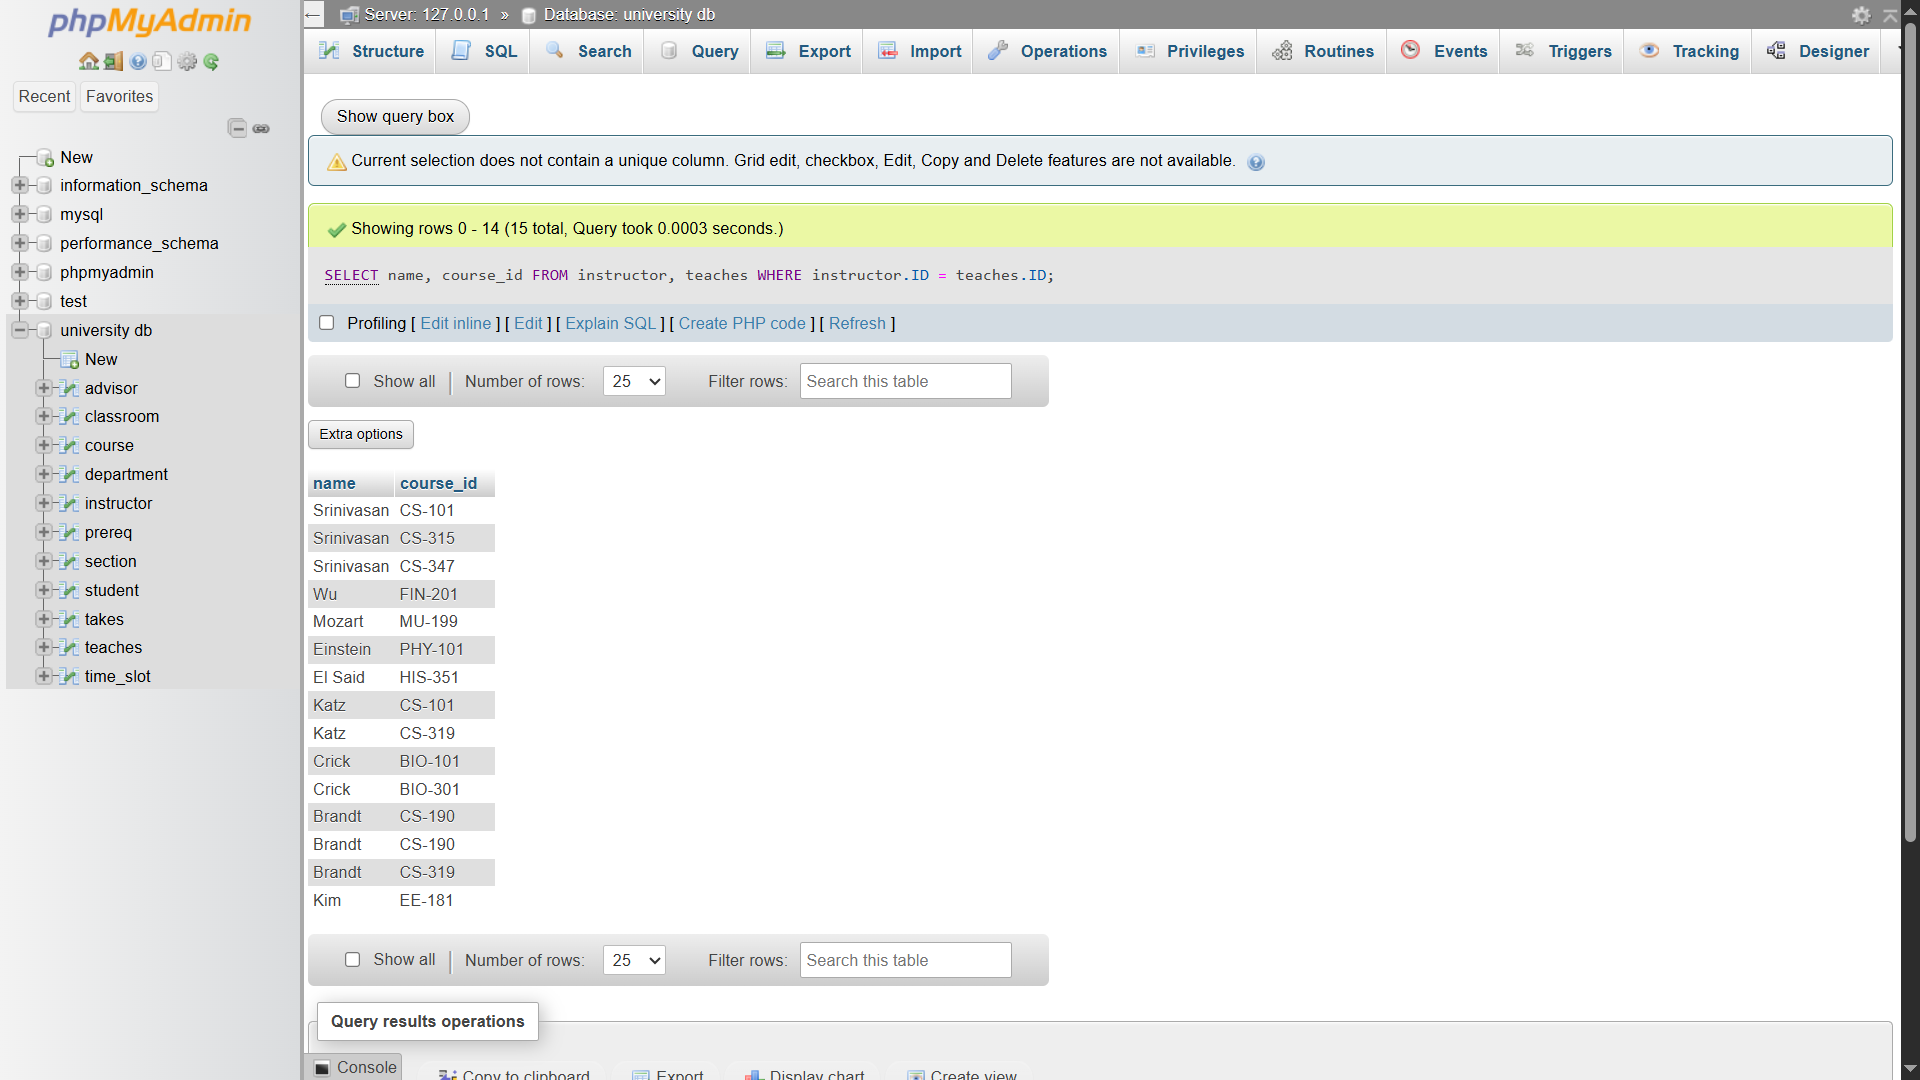
\includegraphics[width=1.0\textwidth]{fig/20.png}
\end{figure}

\begin{verbatim}
SELECT name, course_id 
FROM instructor, teaches 
WHERE instructor.ID = teaches.ID 
AND instructor.dept_name = 'Art';
\end{verbatim}
\begin{figure}[H]
    \centering
    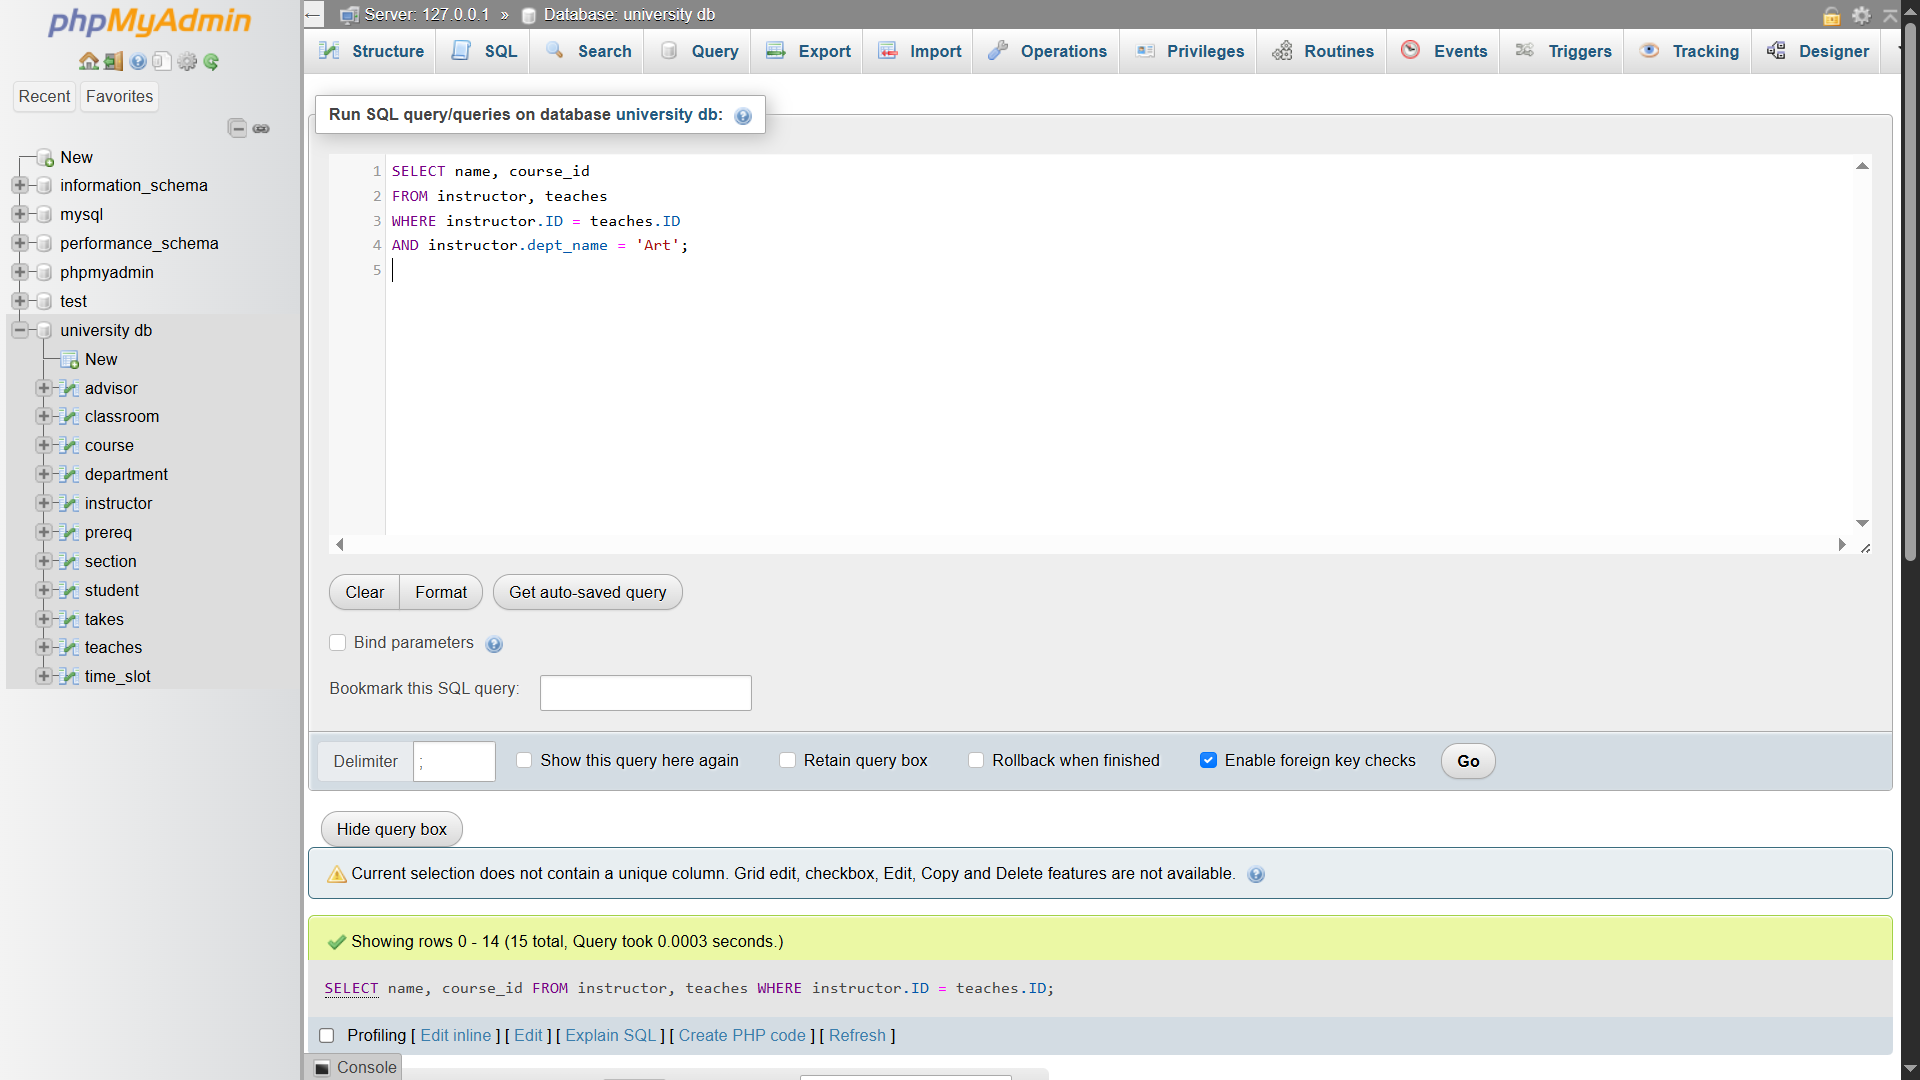
\includegraphics[width=1.0\textwidth]{fig/21.png}
\end{figure}

\begin{figure}[H]
    \centering
    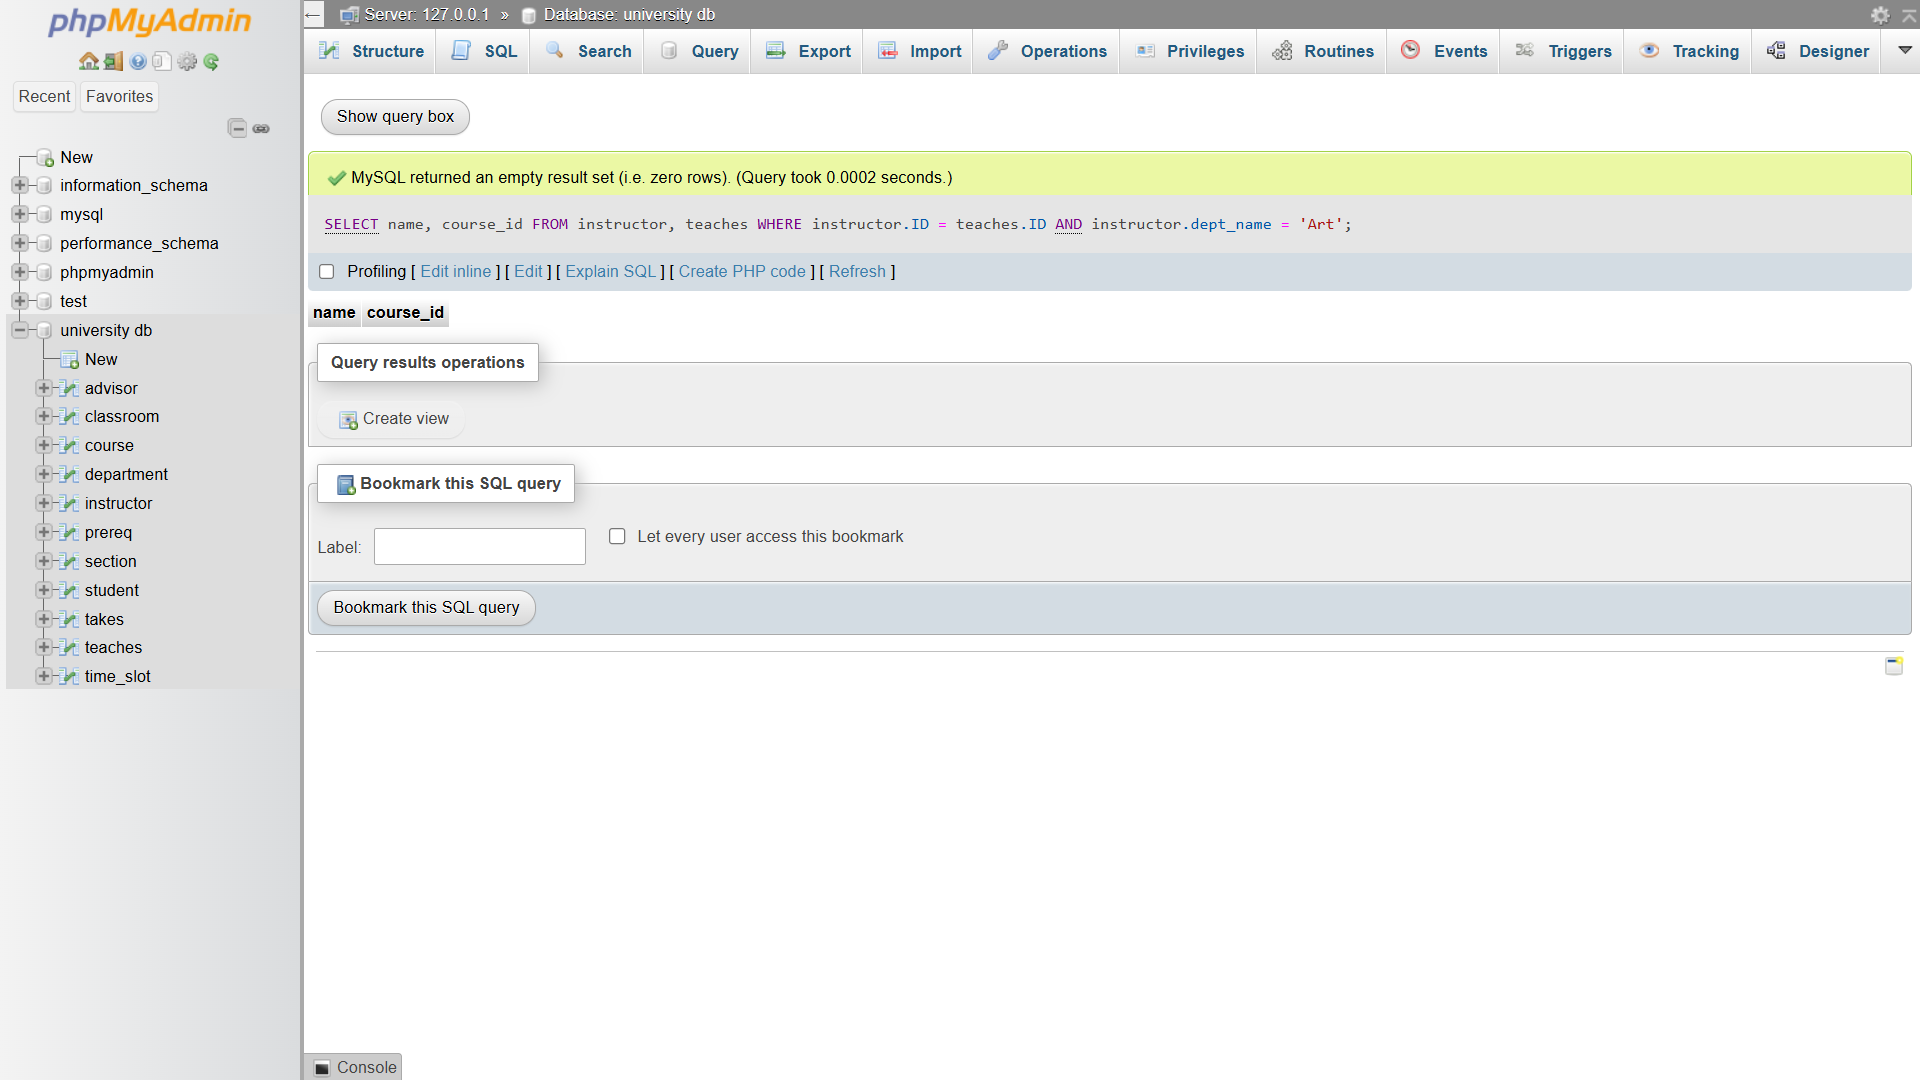
\includegraphics[width=1.0\textwidth]{fig/22.png}
\end{figure}

\begin{verbatim}
SELECT name, course_id 
FROM instructor, teaches 
WHERE instructor.ID = teaches.ID;
\end{verbatim}
\begin{figure}[H]
    \centering
    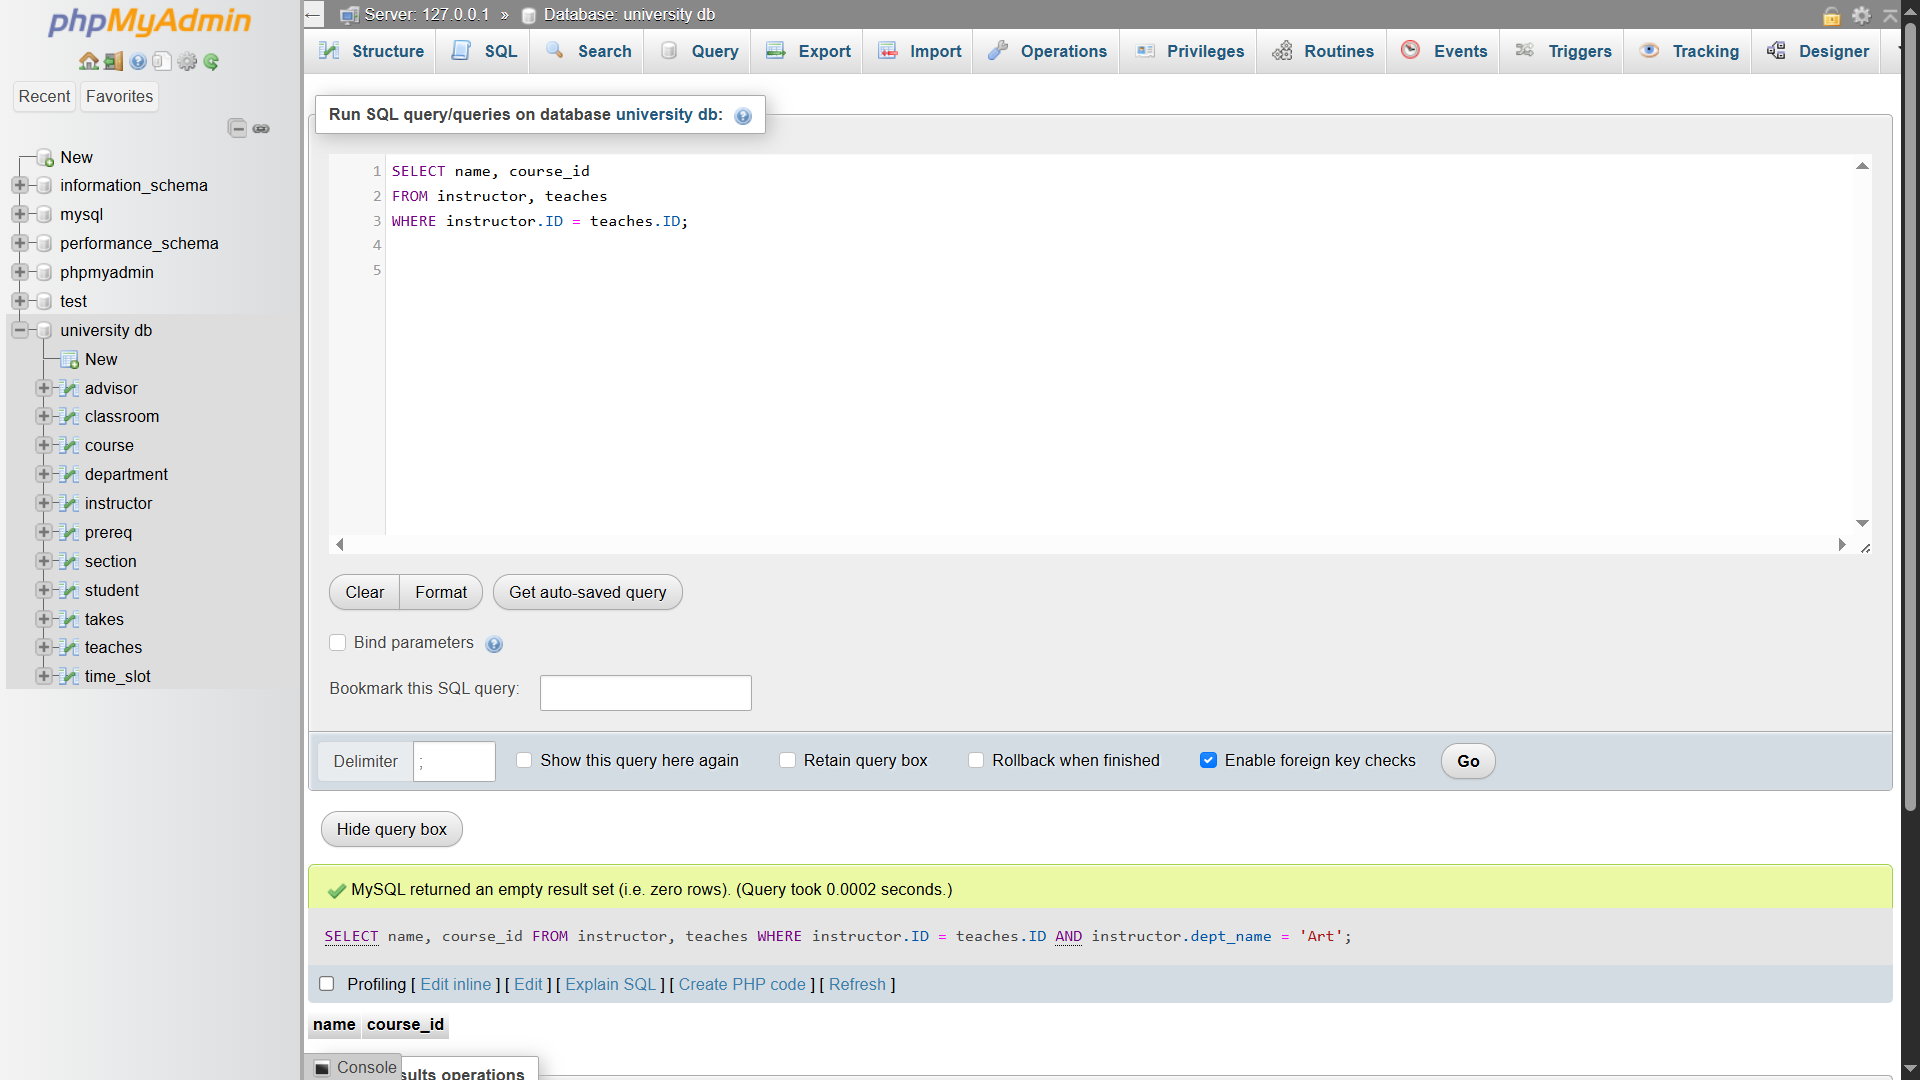
\includegraphics[width=1.0\textwidth]{fig/23.png}
\end{figure}

\begin{figure}[H]
    \centering
    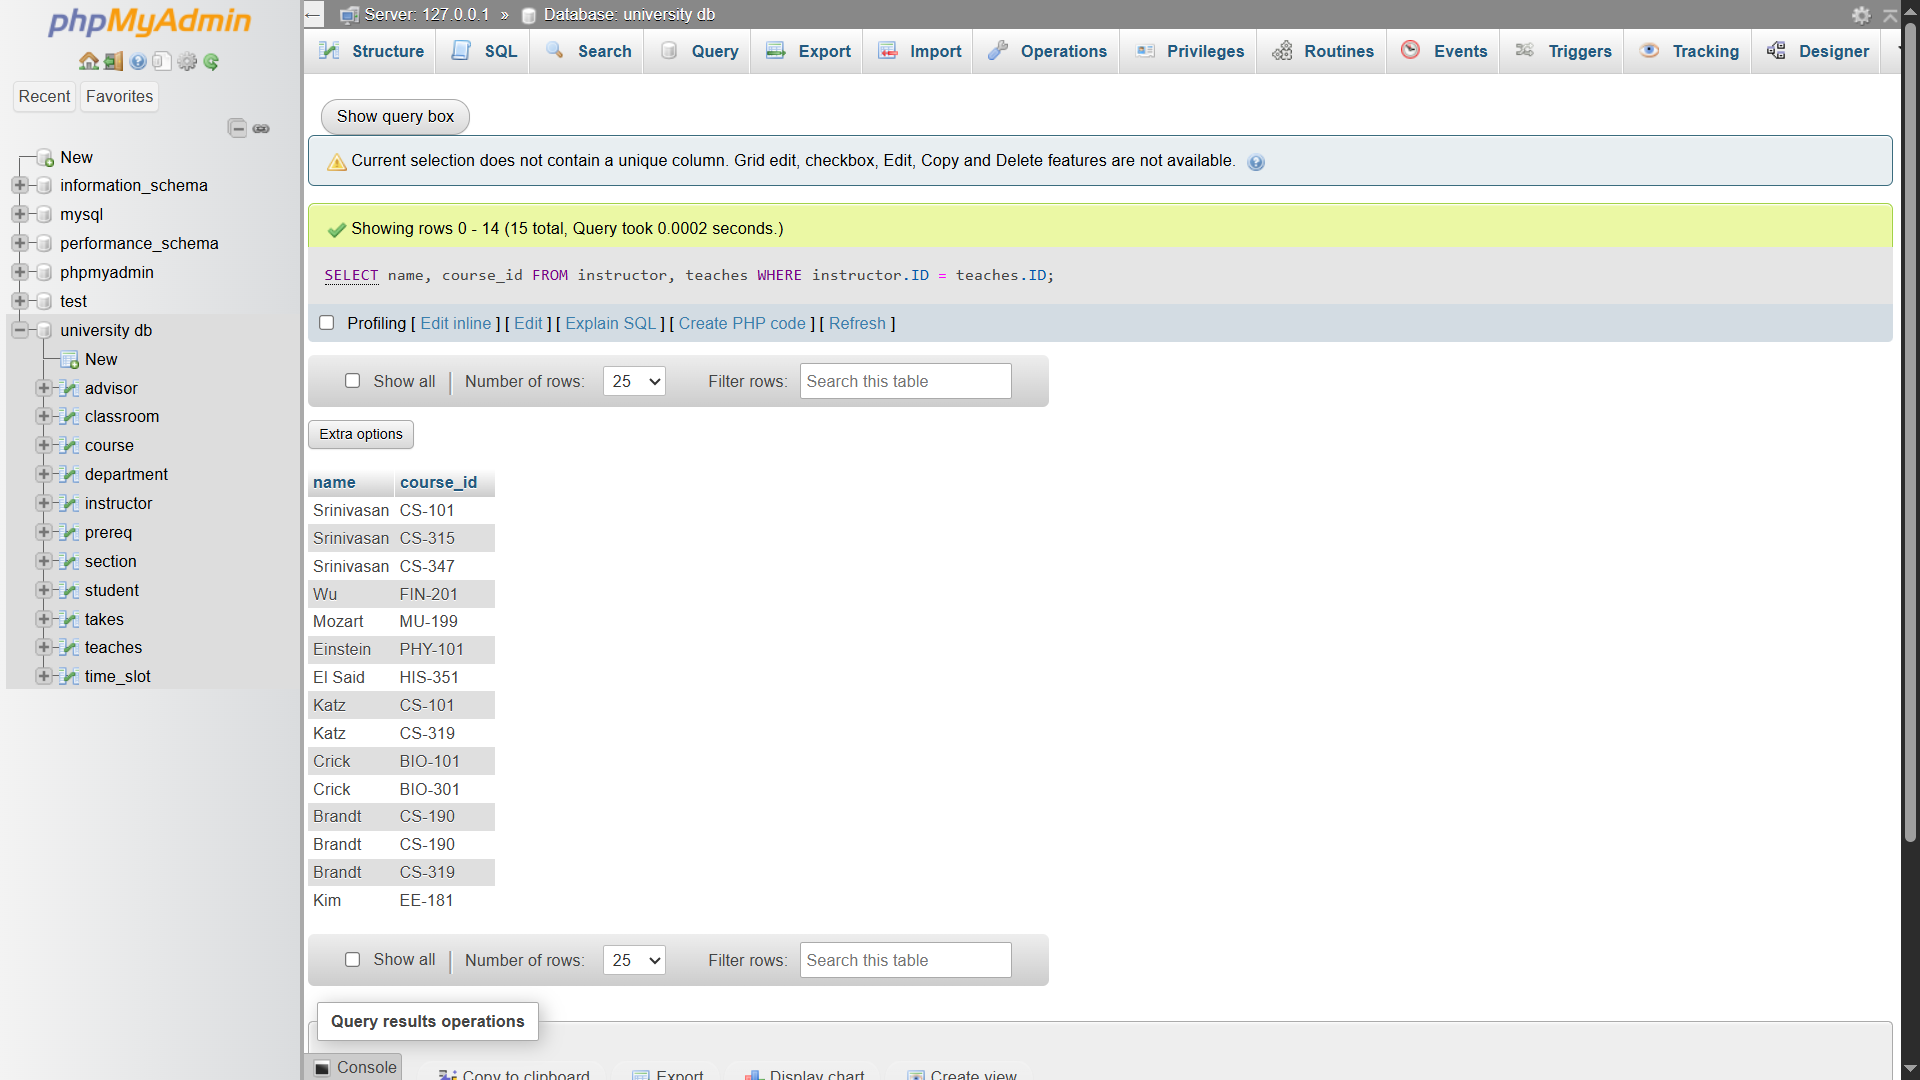
\includegraphics[width=1.0\textwidth]{fig/24.png}
\end{figure}

\begin{verbatim}
SELECT name, course_id 
FROM instructor NATURAL JOIN teaches;
\end{verbatim}
\begin{figure}[H]
    \centering
    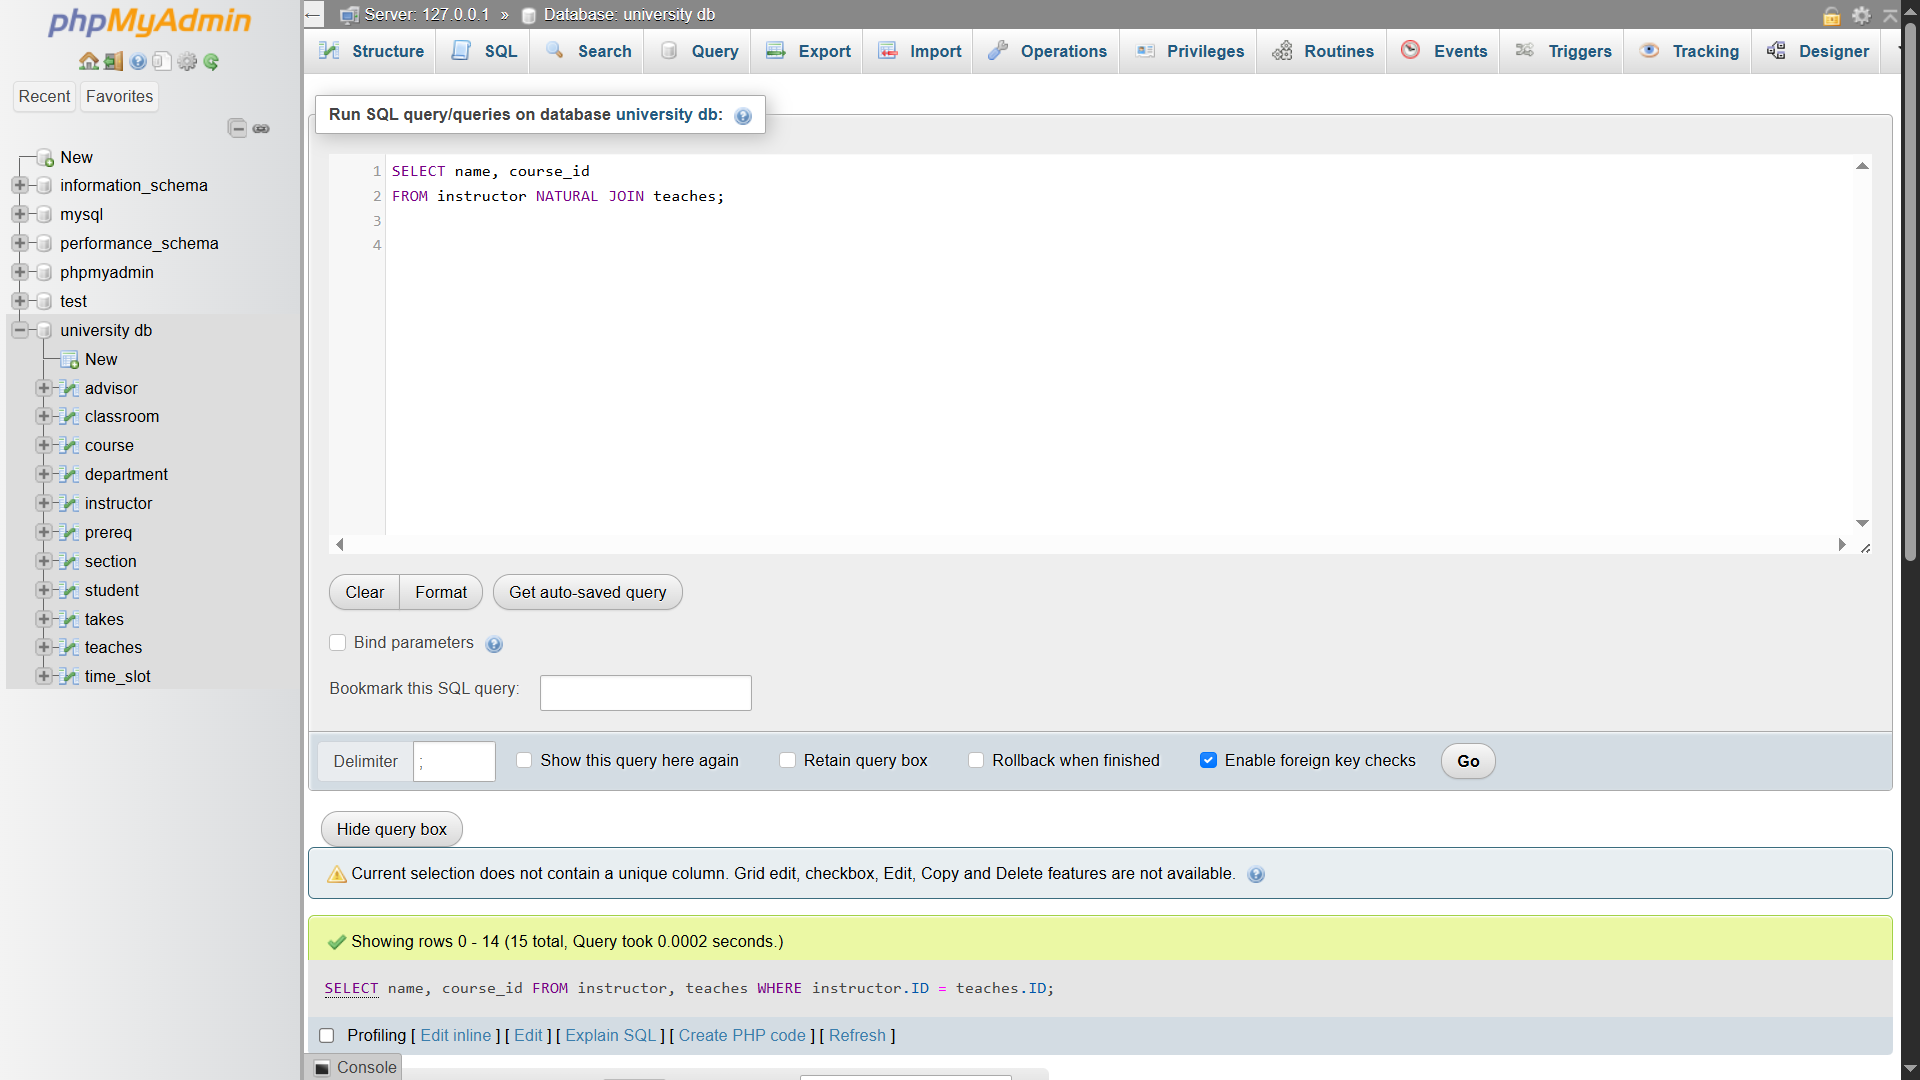
\includegraphics[width=1.0\textwidth]{fig/25.png}
\end{figure}

\begin{figure}[H]
    \centering
    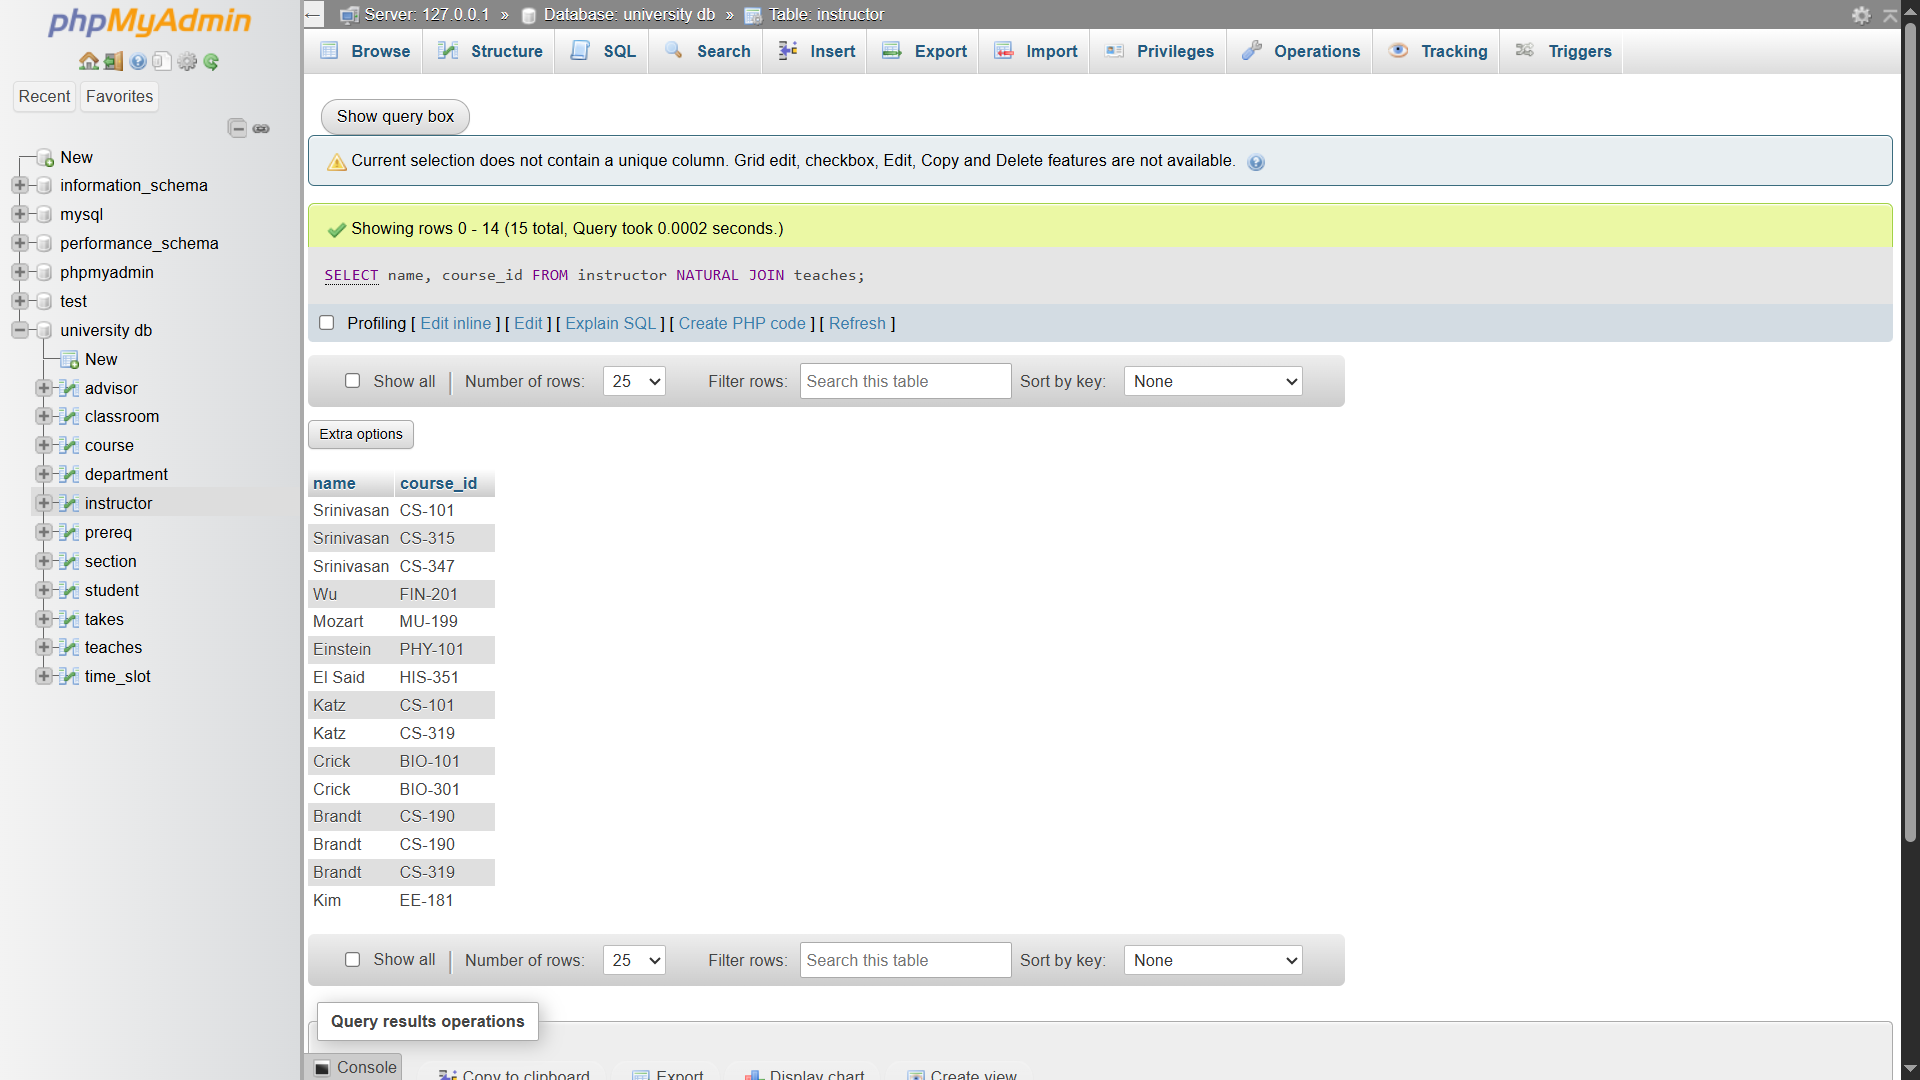
\includegraphics[width=1.0\textwidth]{fig/26.png}
\end{figure}

\begin{verbatim}
SELECT name, title 
FROM instructor NATURAL JOIN teaches, course 
WHERE teaches.course_id = course.course_id;
\end{verbatim}
\begin{figure}[H]
    \centering
    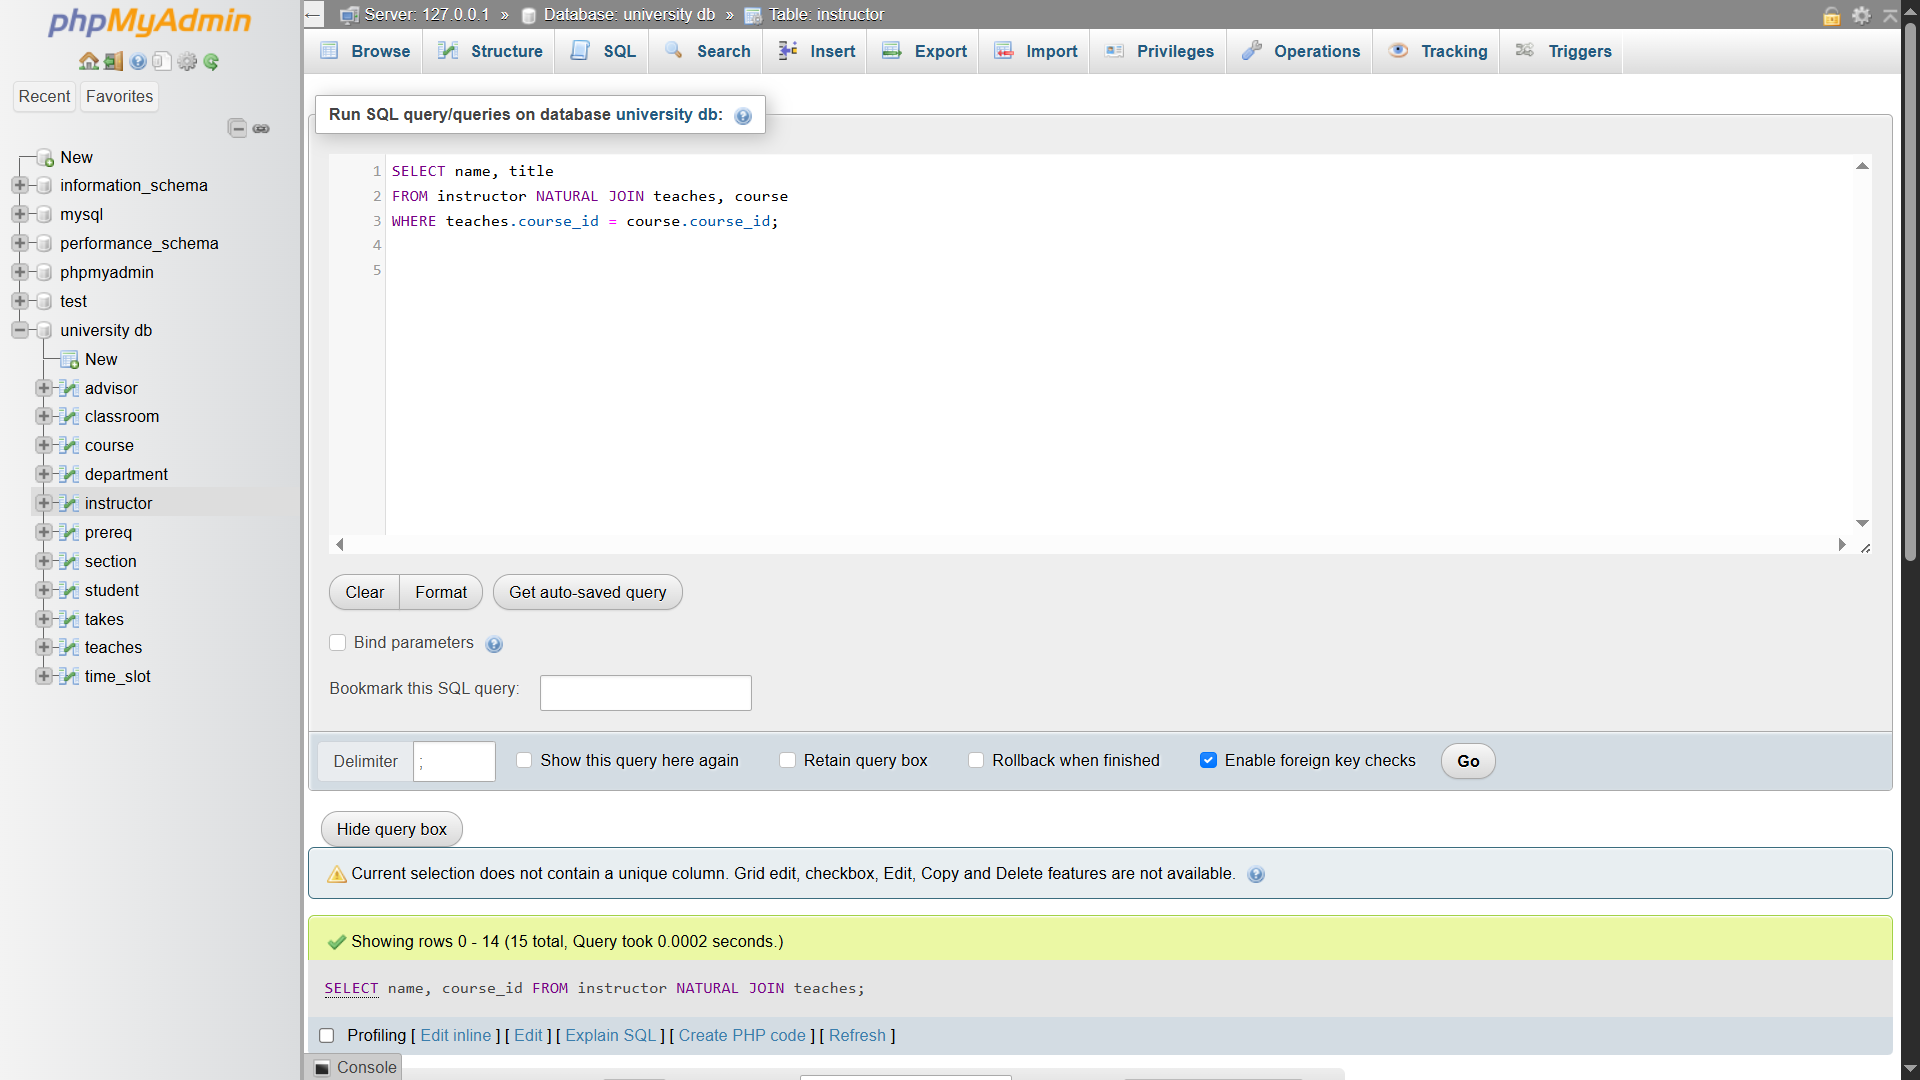
\includegraphics[width=1.0\textwidth]{fig/27.png}
\end{figure}

\begin{figure}[H]
    \centering
    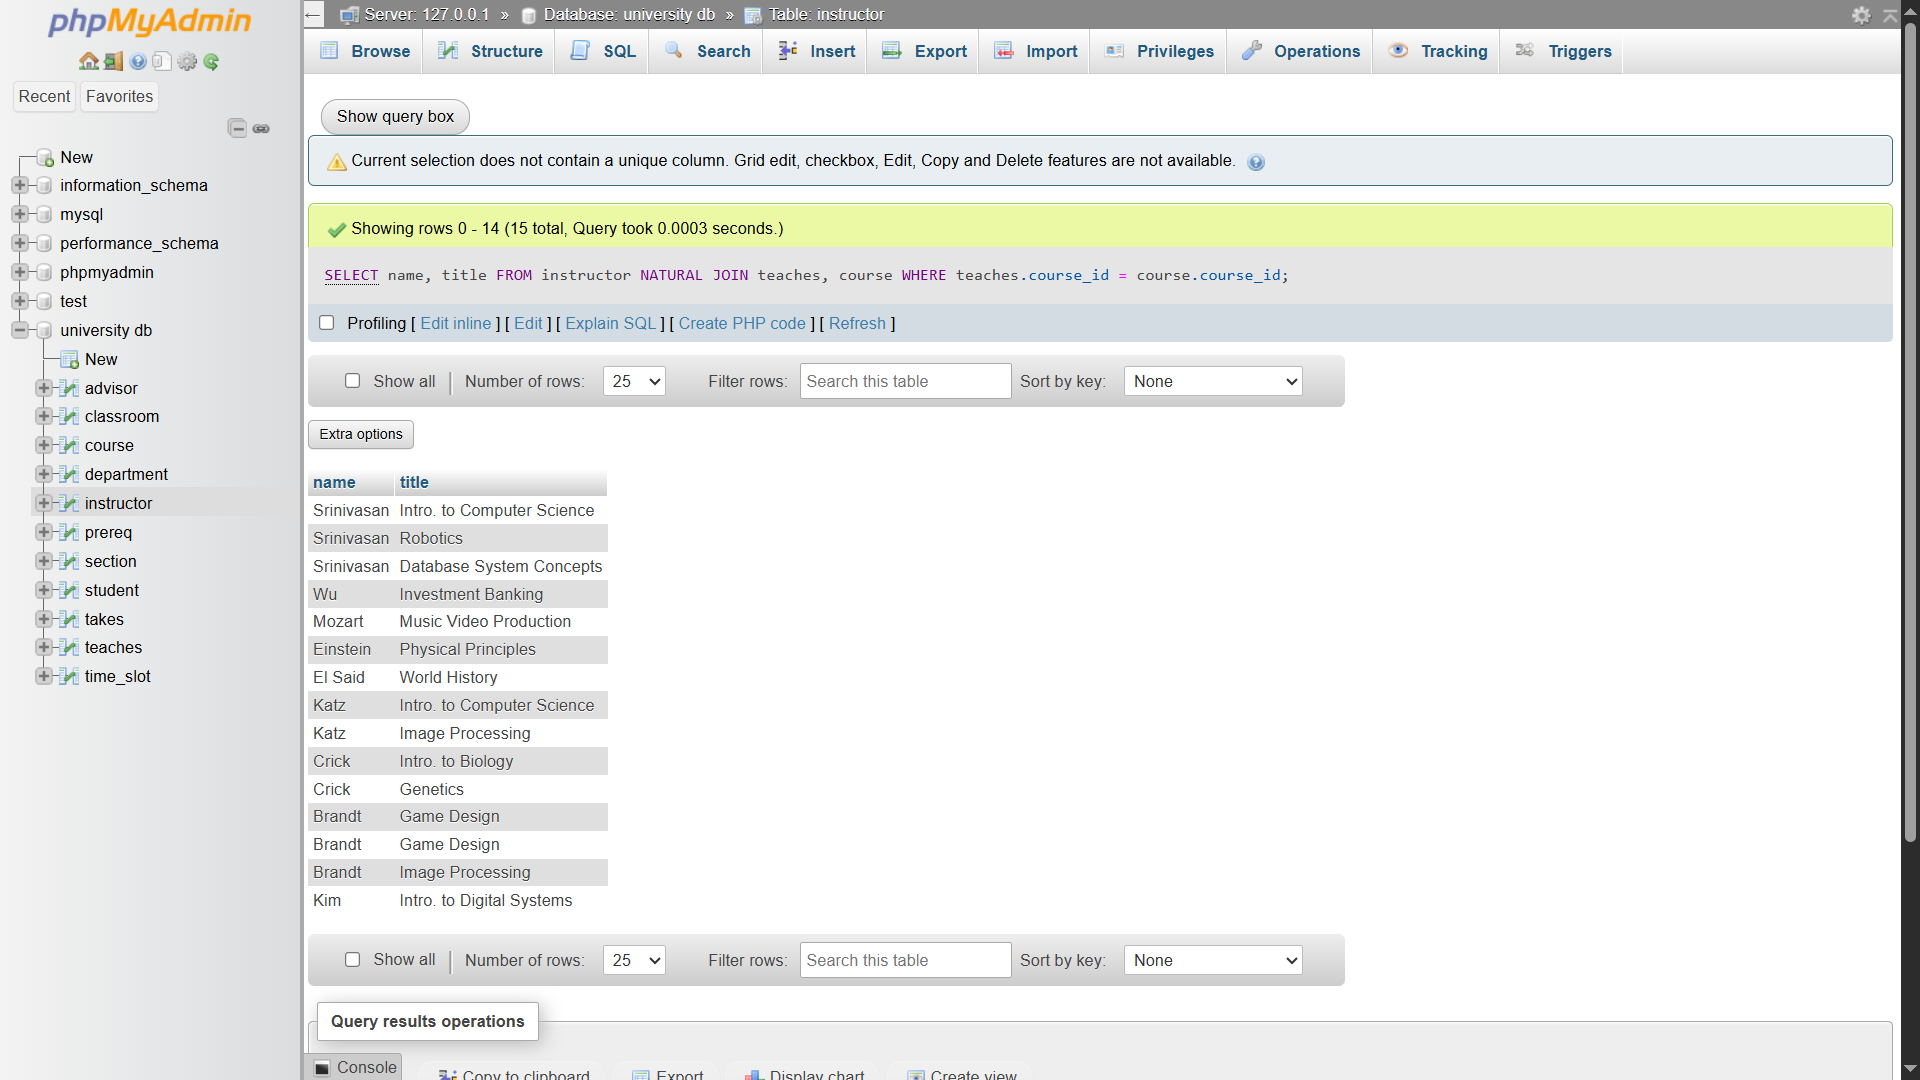
\includegraphics[width=1.0\textwidth]{fig/28.png}
\end{figure}

\begin{verbatim}
SELECT name, title 
FROM instructor NATURAL JOIN teaches 
JOIN course USING (course_id);
\end{verbatim}
\begin{figure}[H]
    \centering
    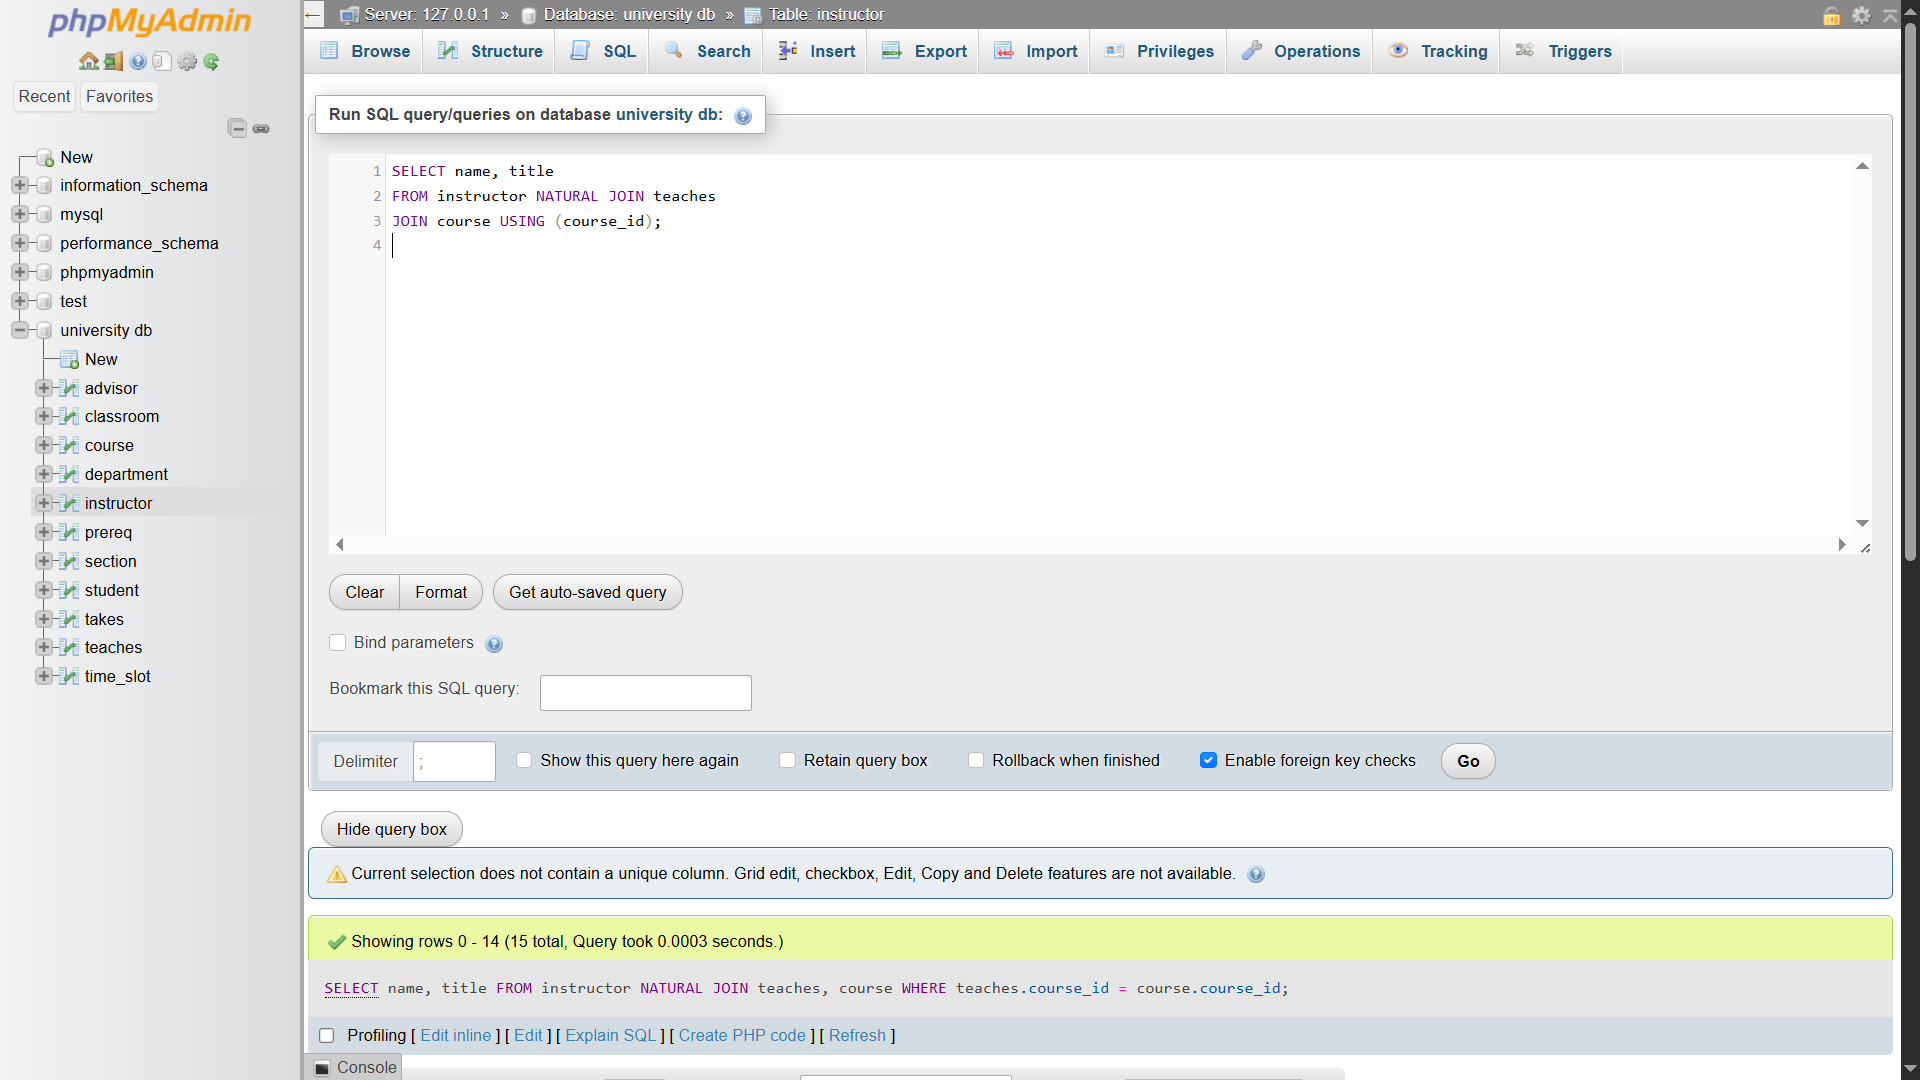
\includegraphics[width=1.0\textwidth]{fig/29.png}
\end{figure}

\begin{figure}[H]
    \centering
    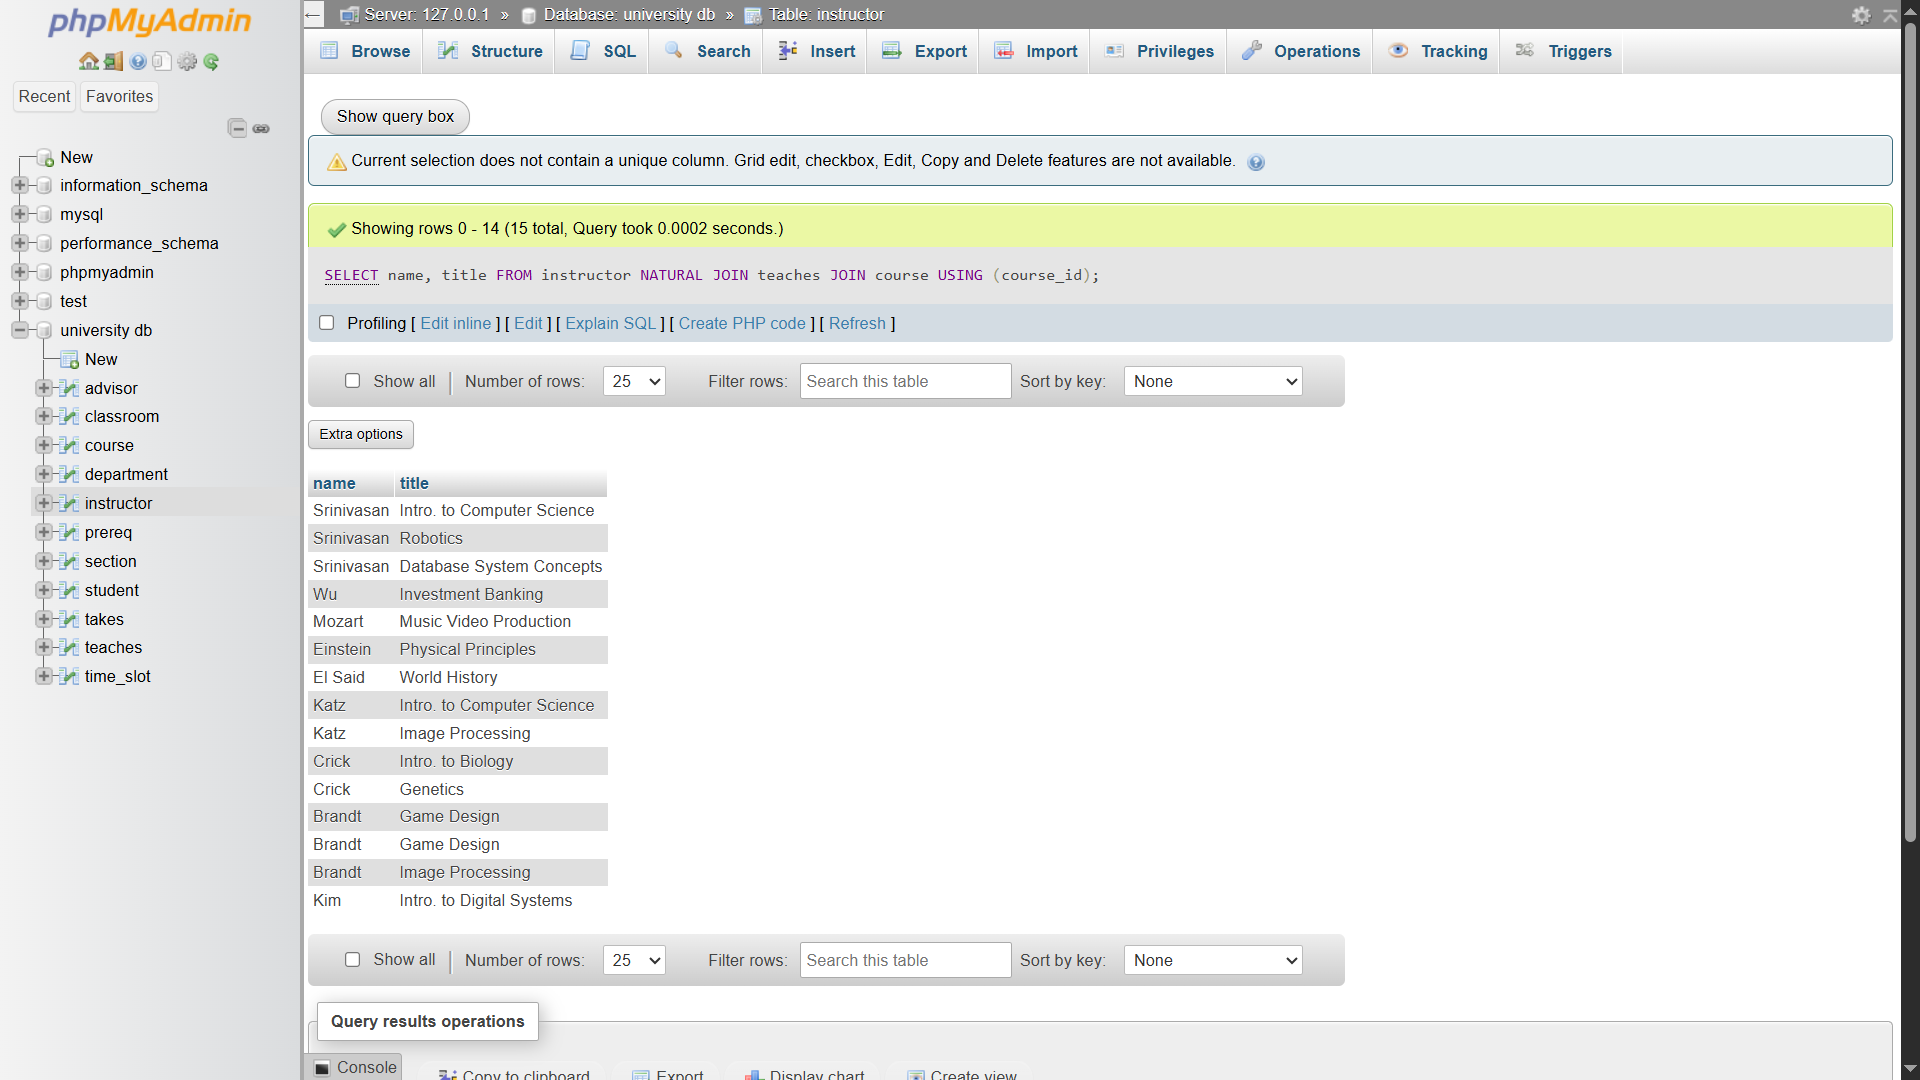
\includegraphics[width=1.0\textwidth]{fig/30.png}
\end{figure}

\begin{verbatim}
SELECT name, title 
FROM instructor NATURAL JOIN teaches 
NATURAL JOIN course;
\end{verbatim}
\begin{figure}
    \centering
    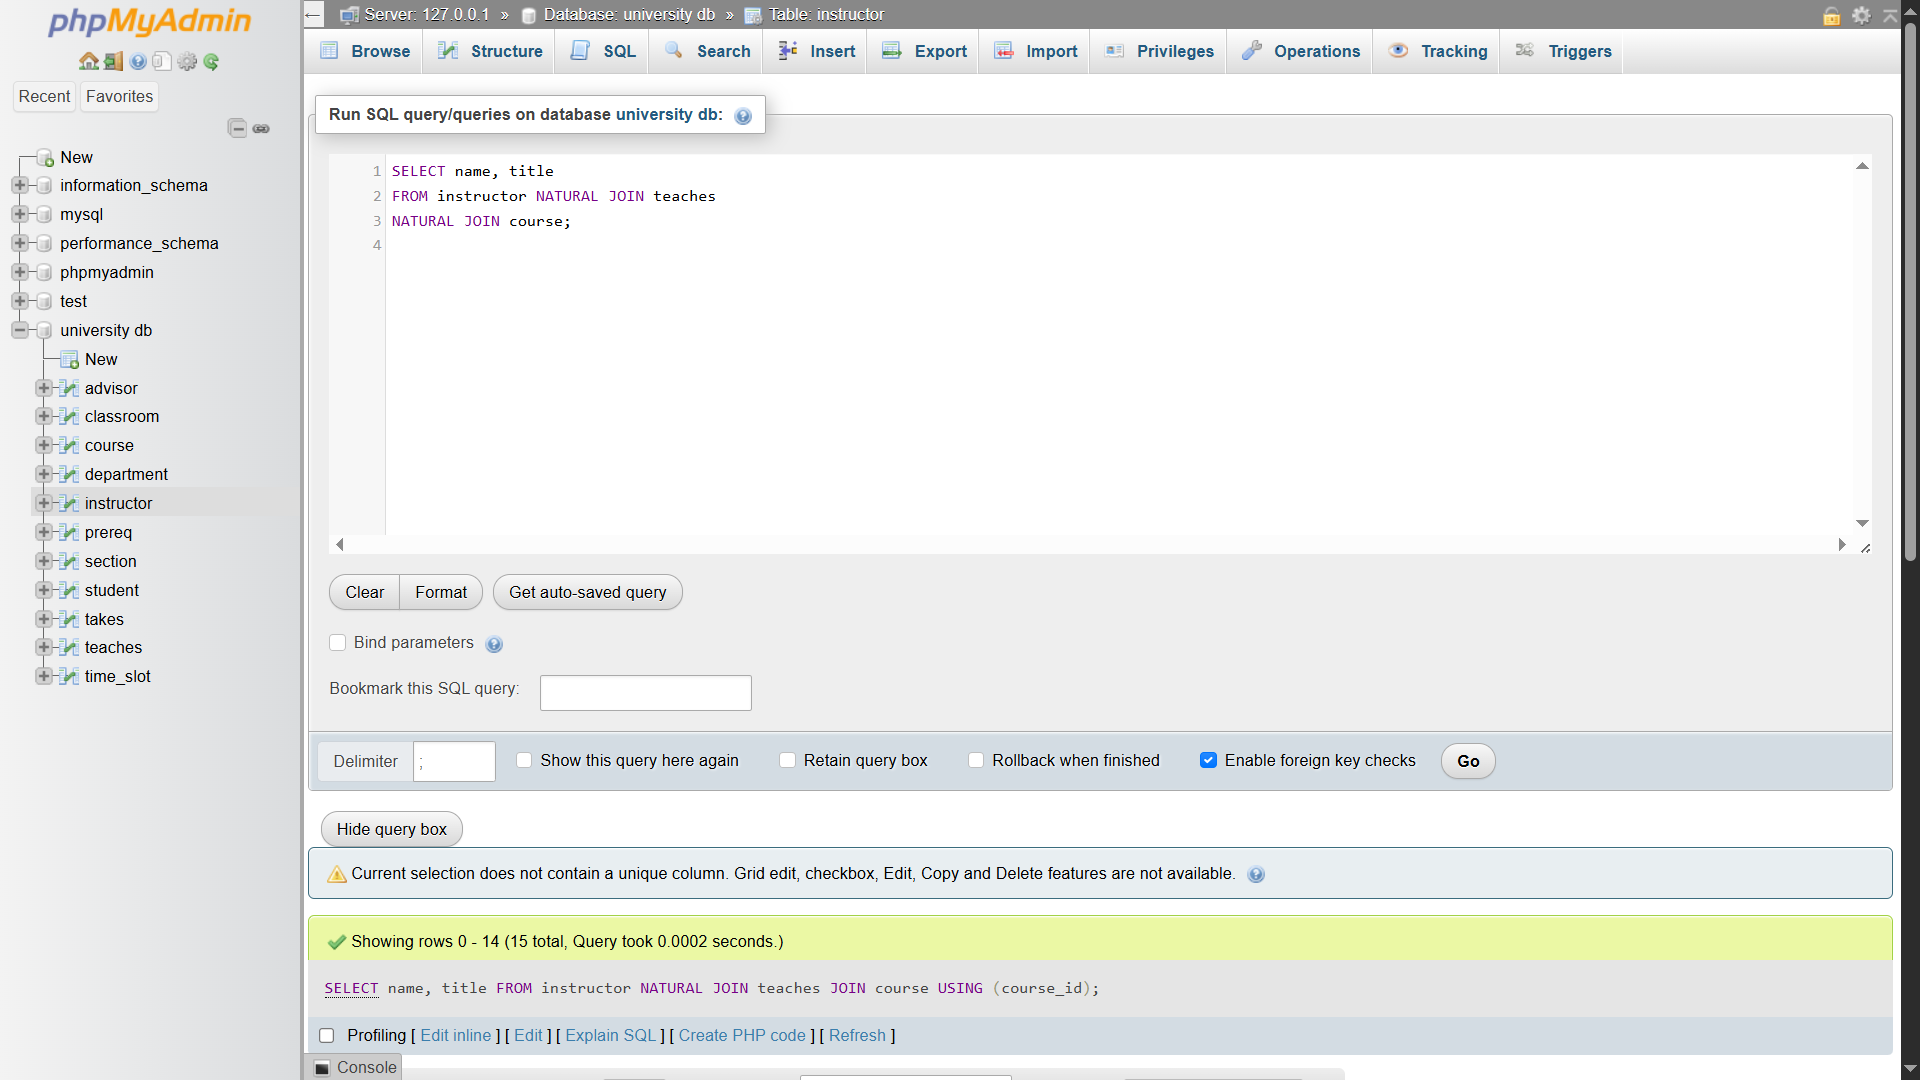
\includegraphics[width=1.0\textwidth]{fig/31.png}
\end{figure}

\begin{figure}[H]
    \centering
    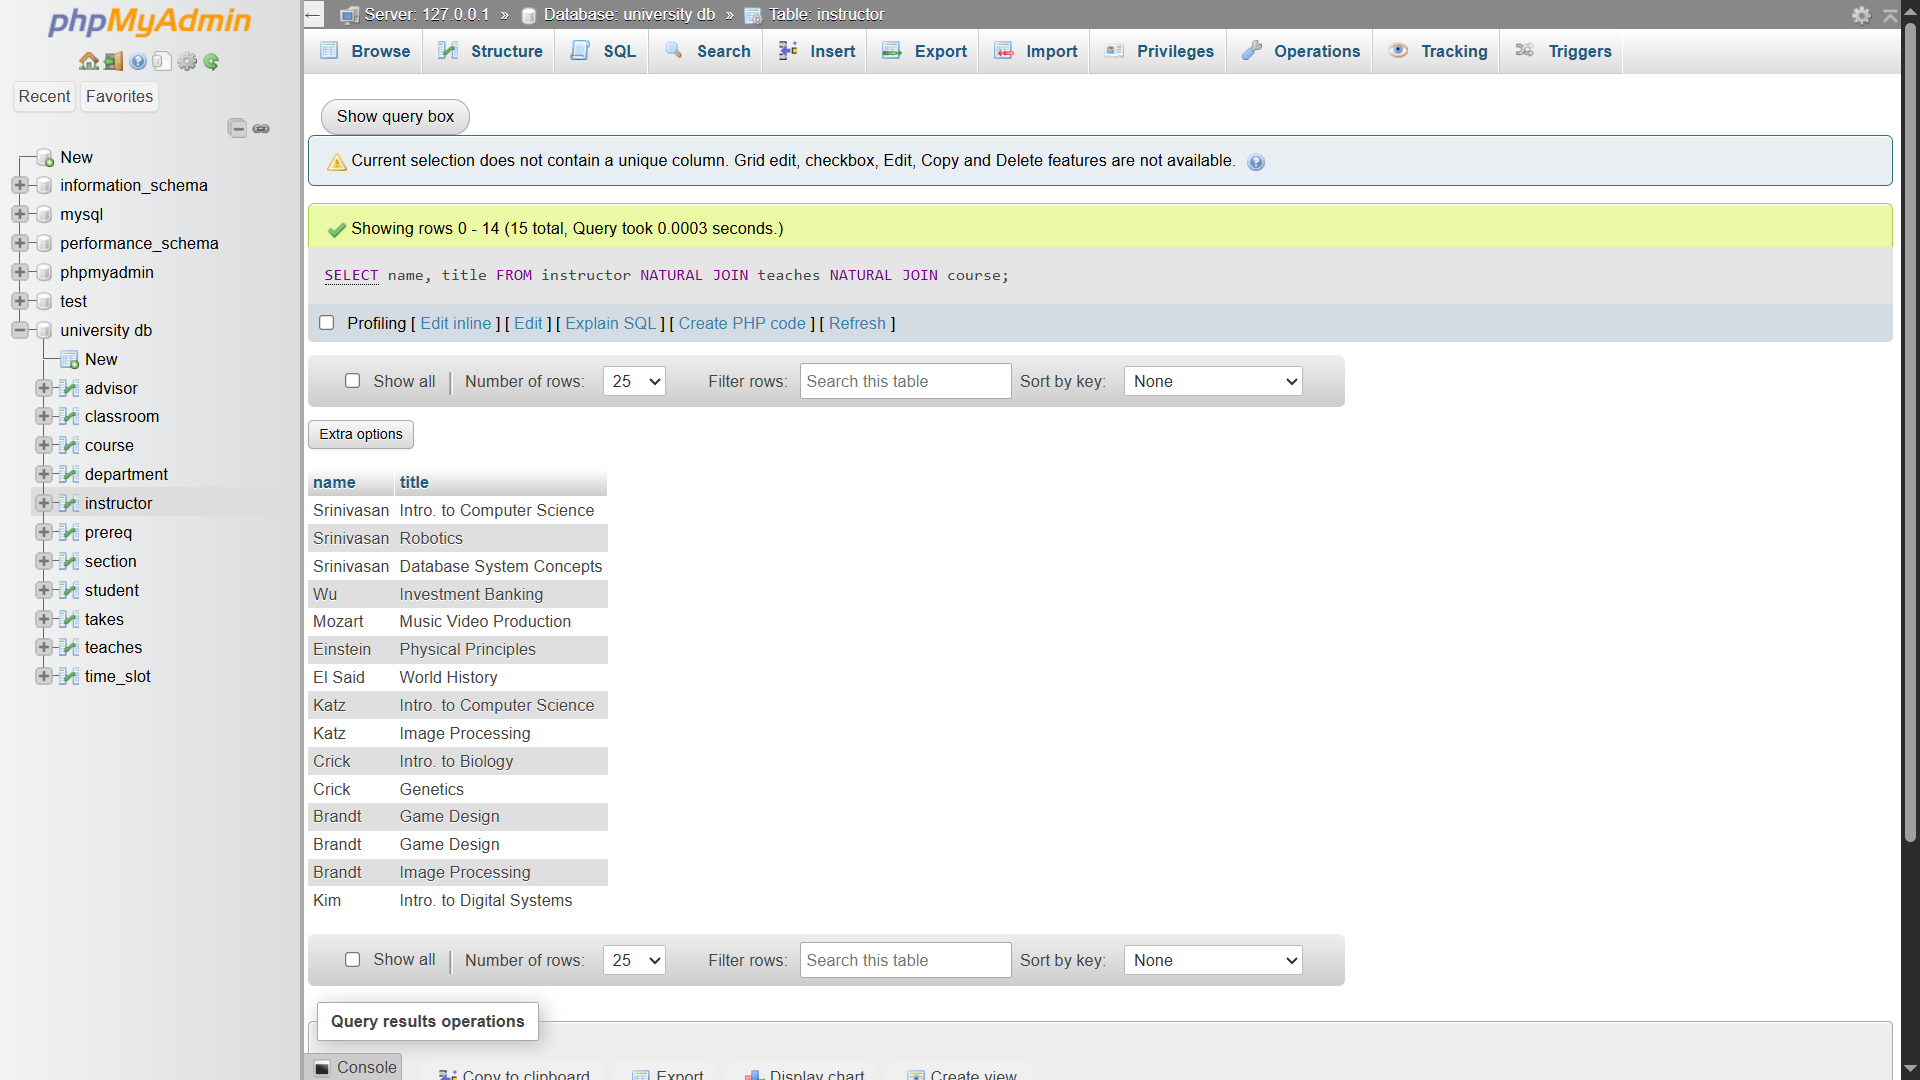
\includegraphics[width=1.0\textwidth]{fig/32.png}
\end{figure}
%%%%%%%%%%%%%%%%%%%%%%%%%%%%%%%%%%%%%%%%%%%%%%%%%%%%%%%%%%%%%%%%%%%%%%%%%%%%%%%%%%%%%%
%moxirboy
%%%%%%%%%%%%%%%%%%%%%%%%%%%%%%%%%%%%%%%%%%%%%%%%%%%%%%%%%%%%%%%%%%%%%%%%%%%%%%%%%%%%%%

\begin{verbatim}
SELECT * FROM instructor NATURAL JOIN teaches, course 
WHERE teaches.course_id = course_id;
\end{verbatim}
\begin{figure}[H]
    \centering
    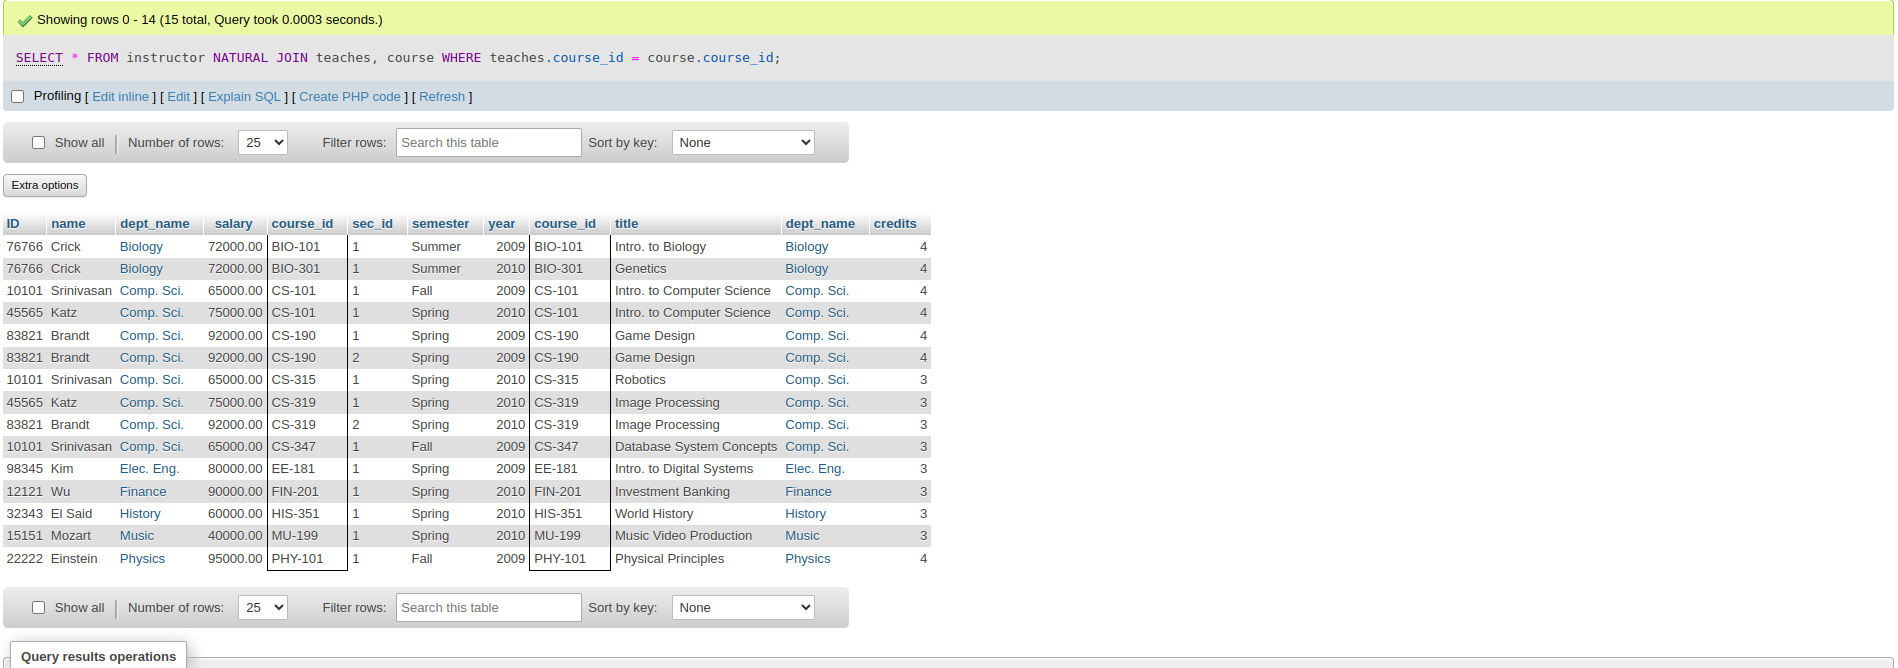
\includegraphics[width=1.0\textwidth]{fig/33.png}
\end{figure}

\begin{verbatim}
SELECT * FROM instructor NATURAL JOIN teaches 
JOIN course USING (course_id);
\end{verbatim}
\begin{figure}[H]
    \centering
    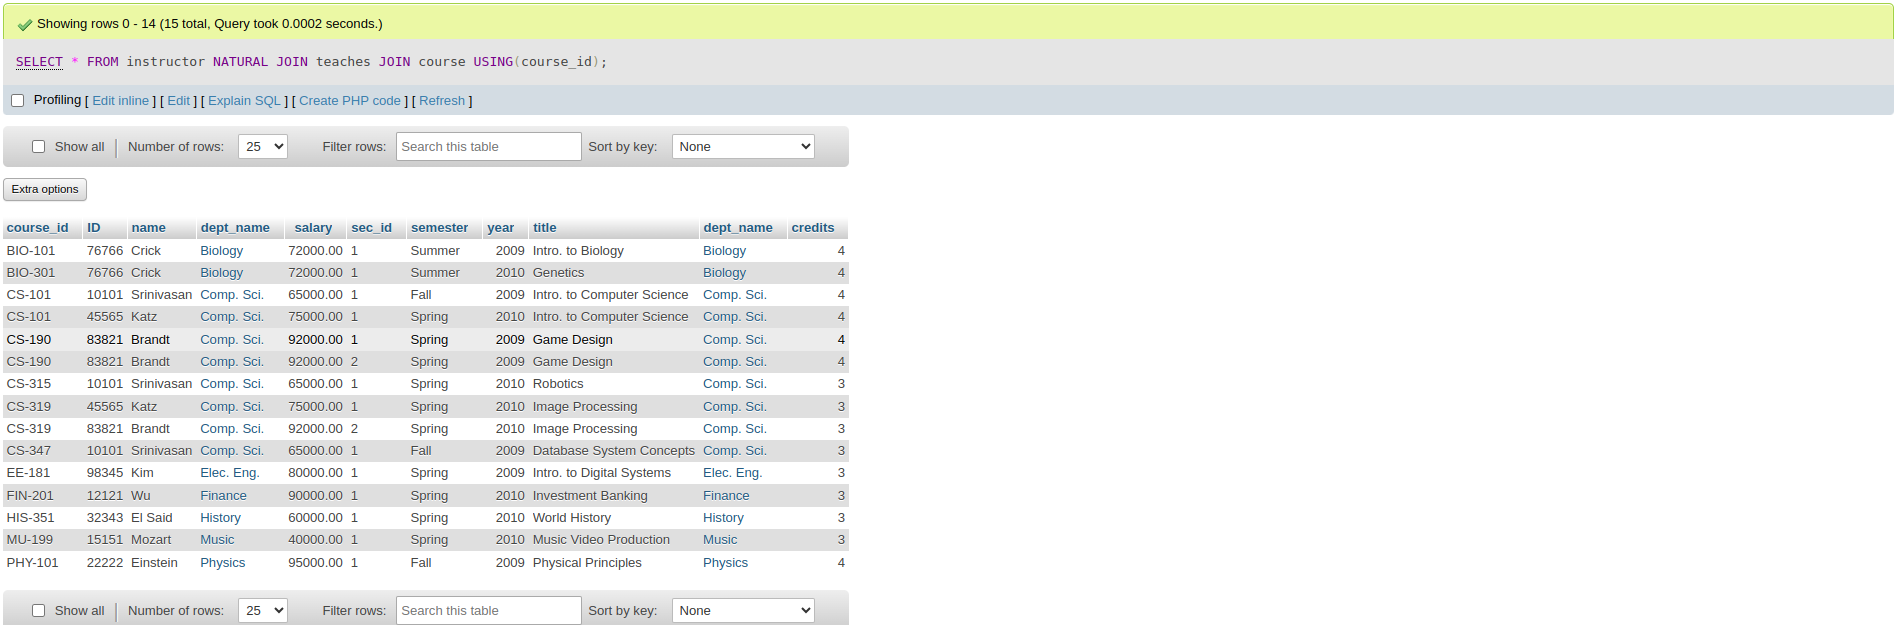
\includegraphics[width=1.0\textwidth]{fig/34.png}
\end{figure}

\begin{verbatim}
SELECT * FROM student JOIN takes ON student.id = takes.id;
\end{verbatim}
\begin{figure}[H]
    \centering
    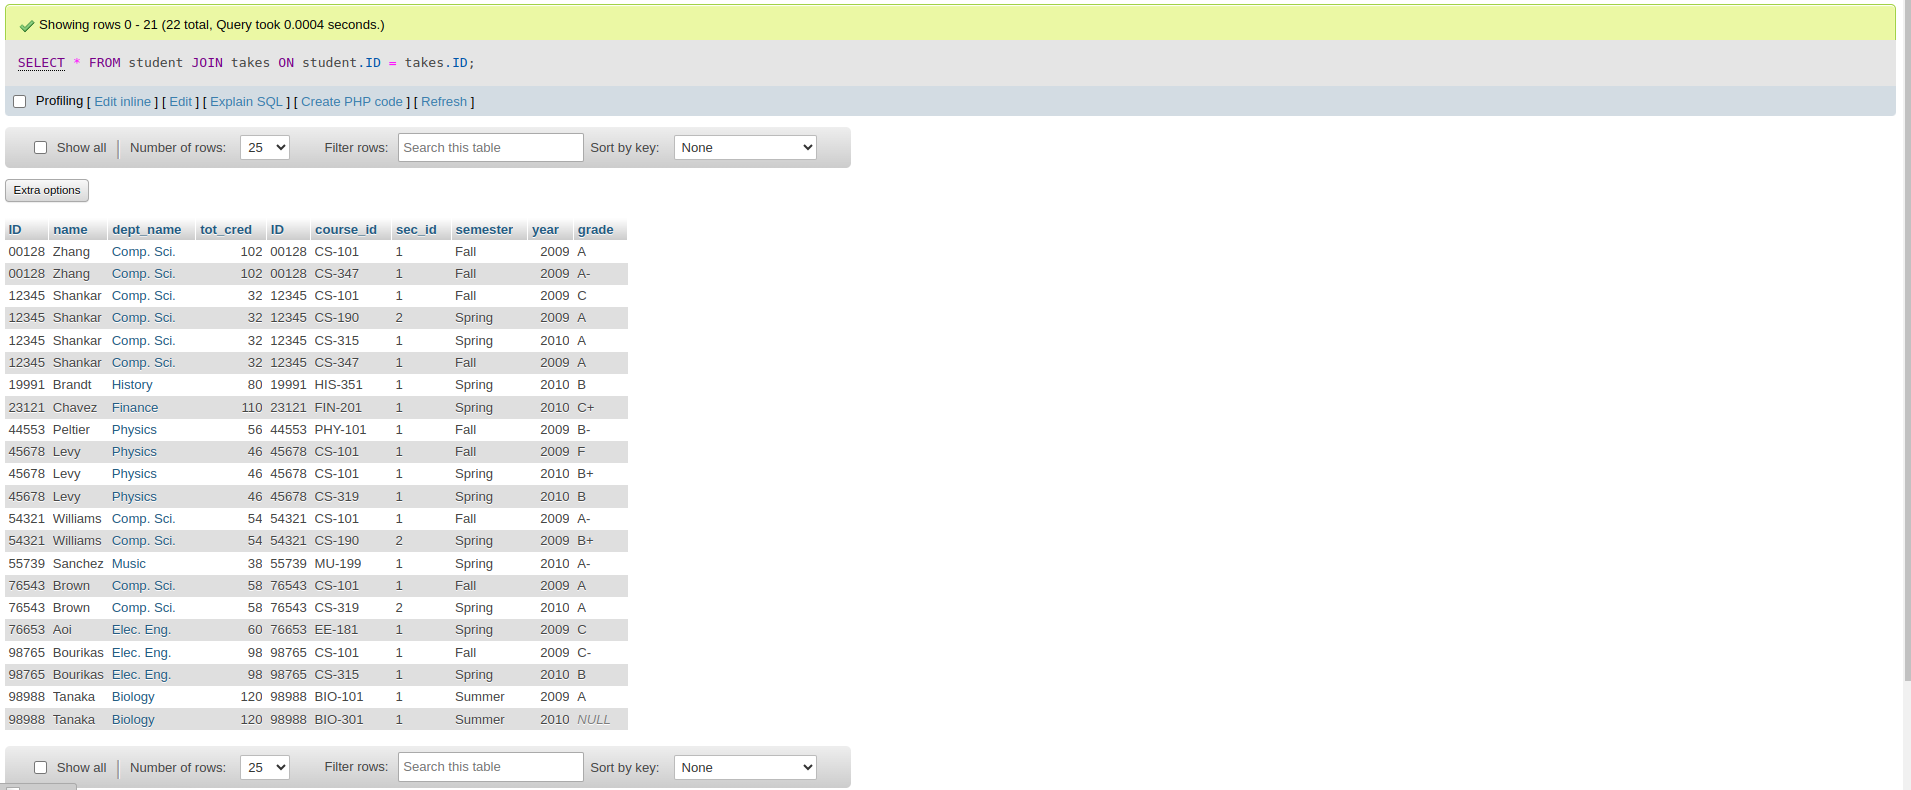
\includegraphics[width=1.0\textwidth]{fig/35.png}
\end{figure}

\begin{verbatim}
SELECT * FROM student NATURAL JOIN takes;
\end{verbatim}
\begin{figure}[H]
    \centering
    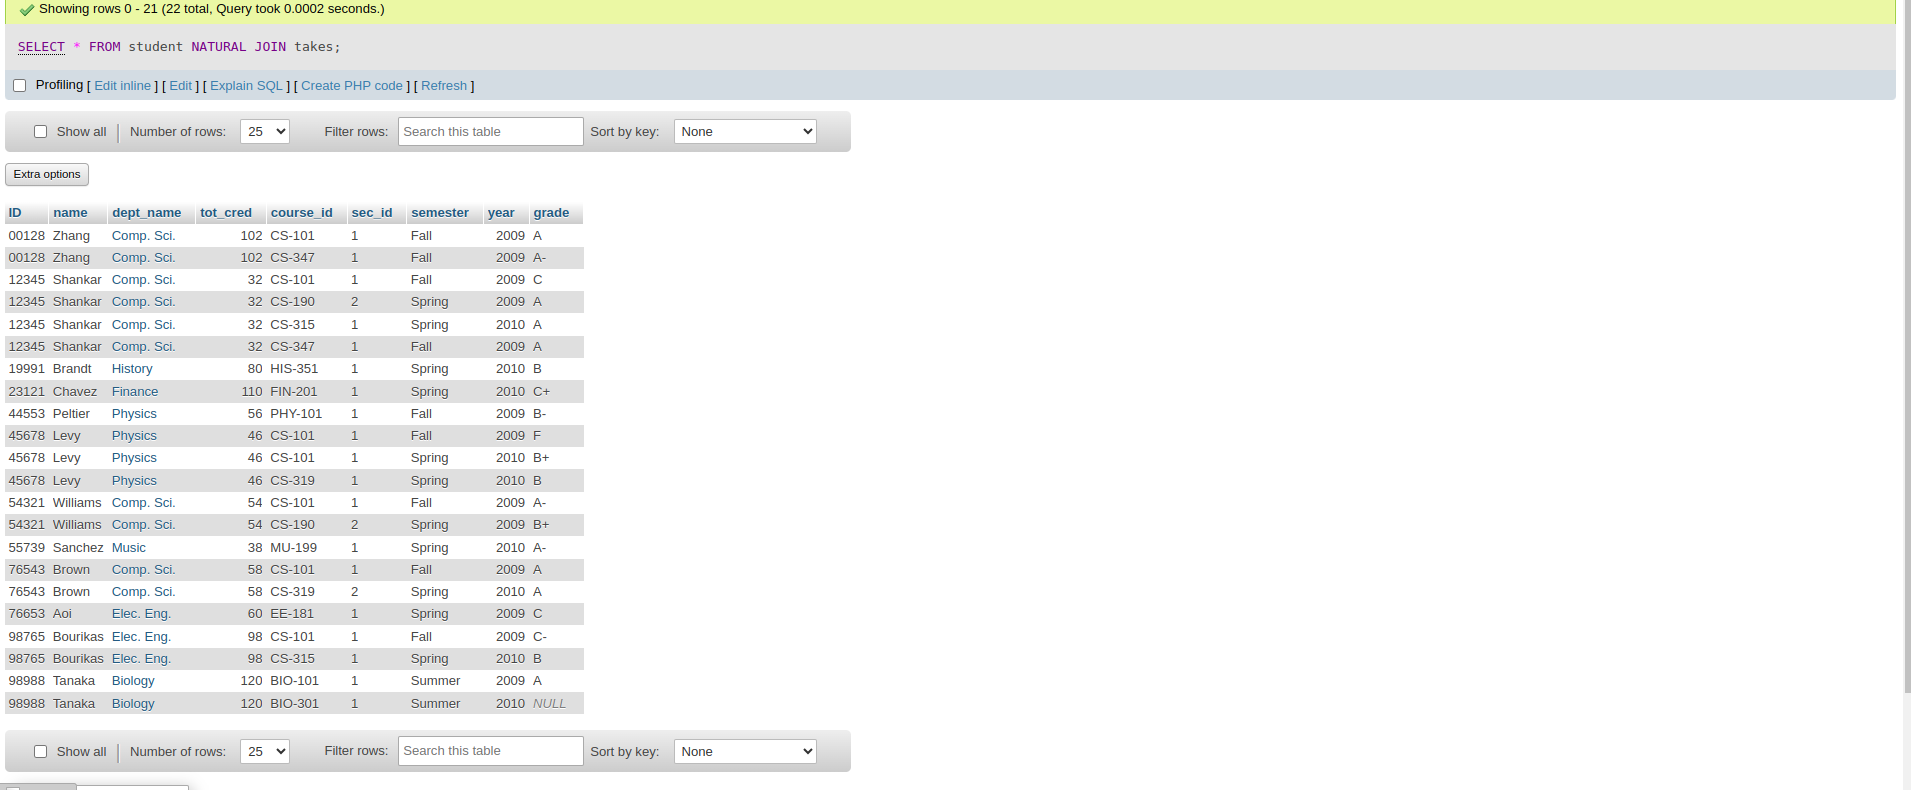
\includegraphics[width=1.0\textwidth]{fig/36.png}
\end{figure}

\begin{verbatim}
SELECT * FROM student JOIN takes ON student.id = takes.id;
\end{verbatim}
\begin{figure}[H]
    \centering
    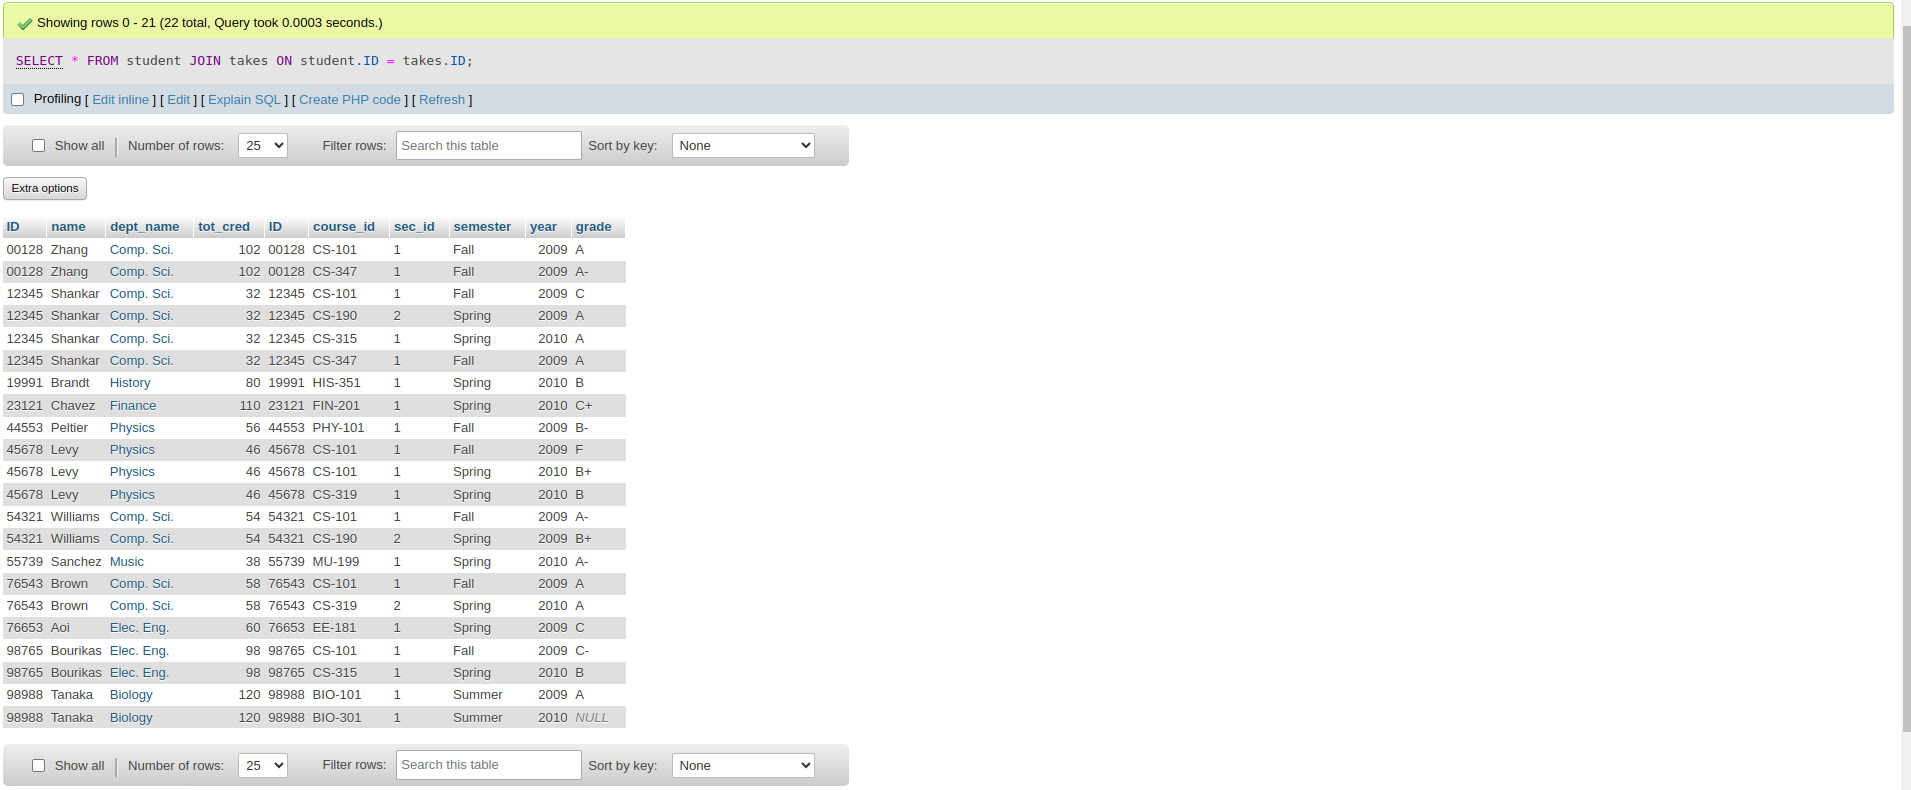
\includegraphics[width=1.0\textwidth]{fig/37.png}
\end{figure}

\begin{verbatim}
SELECT * FROM student, takes 
WHERE student.ID = takes.ID;
\end{verbatim}
\begin{figure}[H]
    \centering
    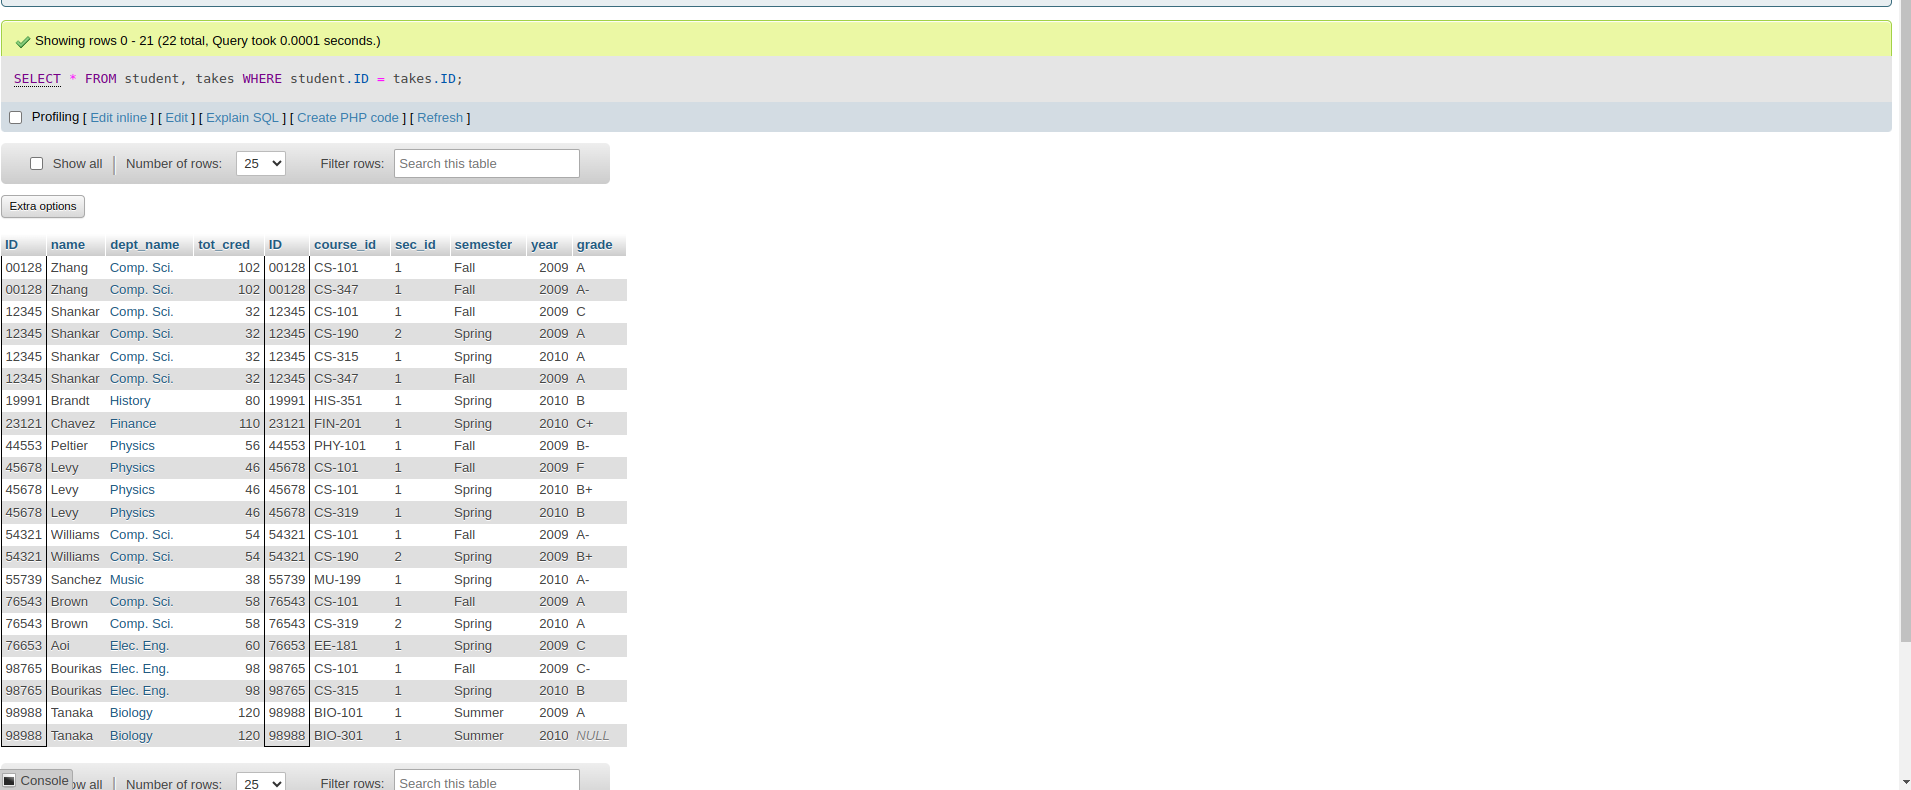
\includegraphics[width=1.0\textwidth]{fig/38.png}
\end{figure}

\begin{verbatim}
SELECT student.ID, student.NAME, student.dept_name, student.tot_cred, 
       takes.course_id, takes.sec_id, takes.semester, takes.YEAR, takes.grade 
FROM student 
JOIN takes ON student.ID = takes.ID;
\end{verbatim}
\begin{figure}[H]
    \centering
    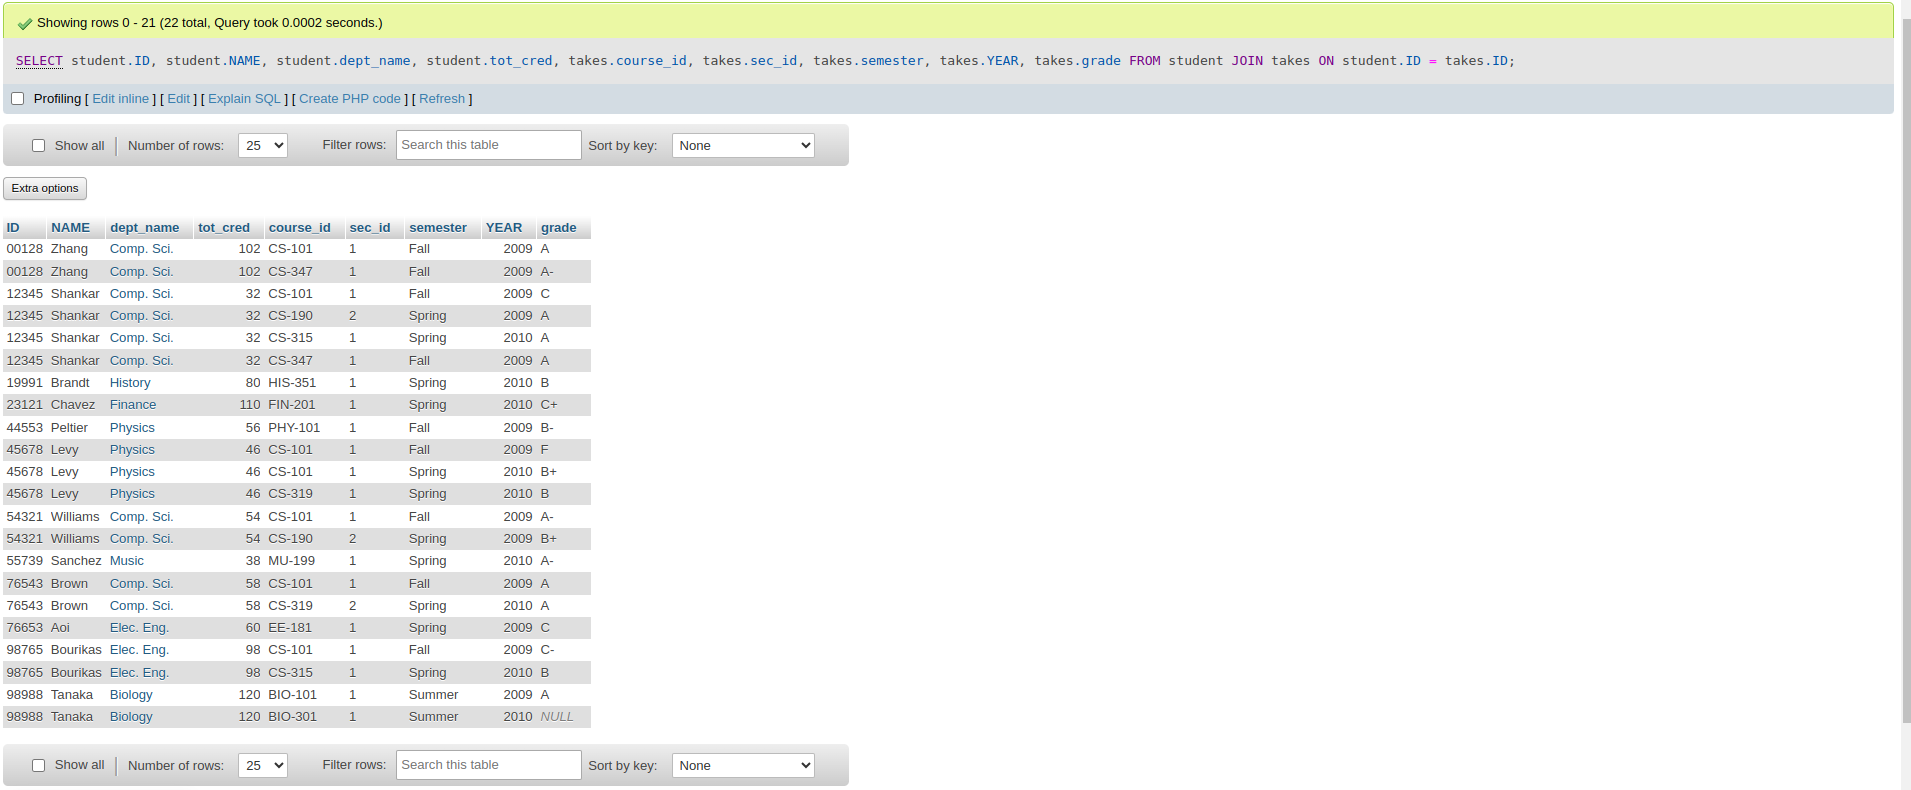
\includegraphics[width=1.0\textwidth]{fig/39.png}
\end{figure}

\begin{verbatim}
SELECT course_id FROM section WHERE semester = 'FALL';
\end{verbatim}
\begin{figure}[H]
    \centering
    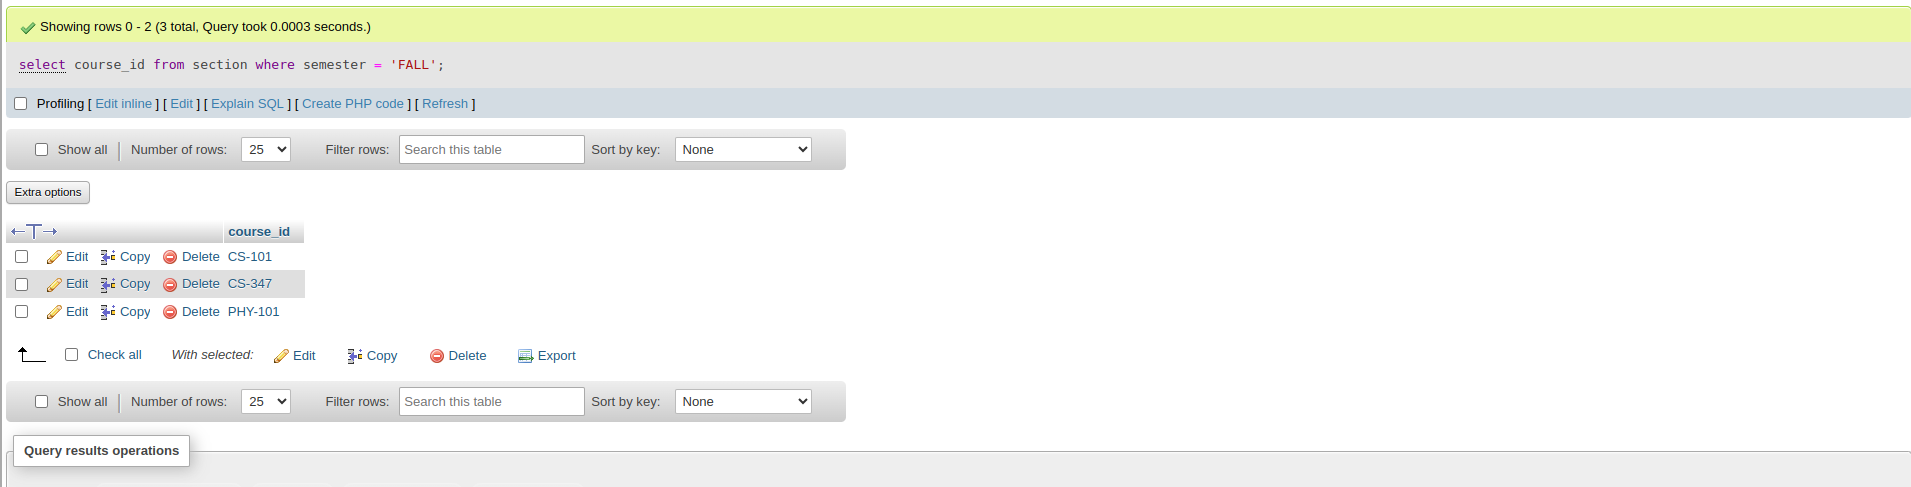
\includegraphics[width=1.0\textwidth]{fig/40.png}
\end{figure}

\begin{verbatim}
SELECT course_id FROM section WHERE semester = 'Spring' AND year = '2010';
\end{verbatim}
\begin{figure}[H]
    \centering
    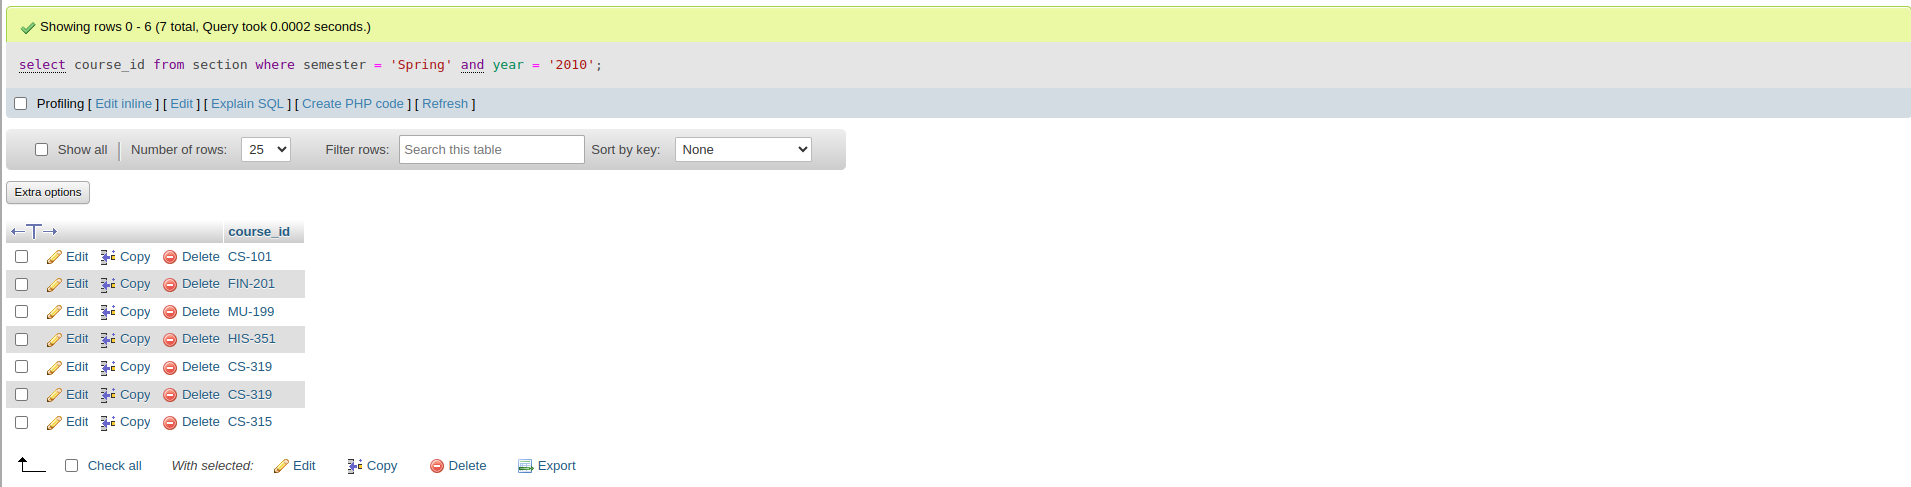
\includegraphics[width=1.0\textwidth]{fig/41.png}
\end{figure}

\begin{verbatim}
(SELECT course_id FROM section WHERE semester = 'FALL' AND YEAR = '2009')
UNION
(SELECT course_id FROM section WHERE semester = 'Spring' AND YEAR = '2010');
\end{verbatim}
\begin{figure}[H]
    \centering
    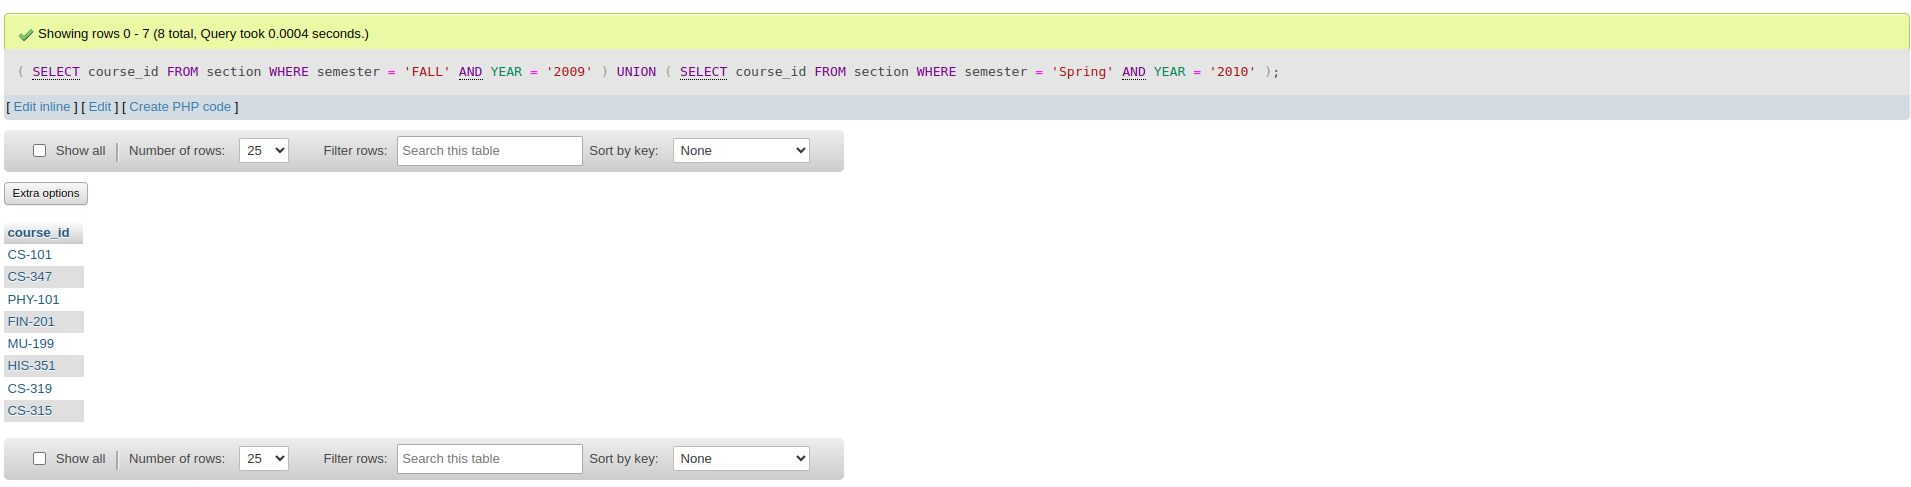
\includegraphics[width=1.0\textwidth]{fig/42.png}
\end{figure}

\begin{verbatim}
SELECT course_id 
FROM section 
WHERE (semester = 'FALL' AND YEAR = '2009') 
   OR (semester = 'Spring' AND YEAR = '2010');
\end{verbatim}
\begin{figure}[H]
    \centering
    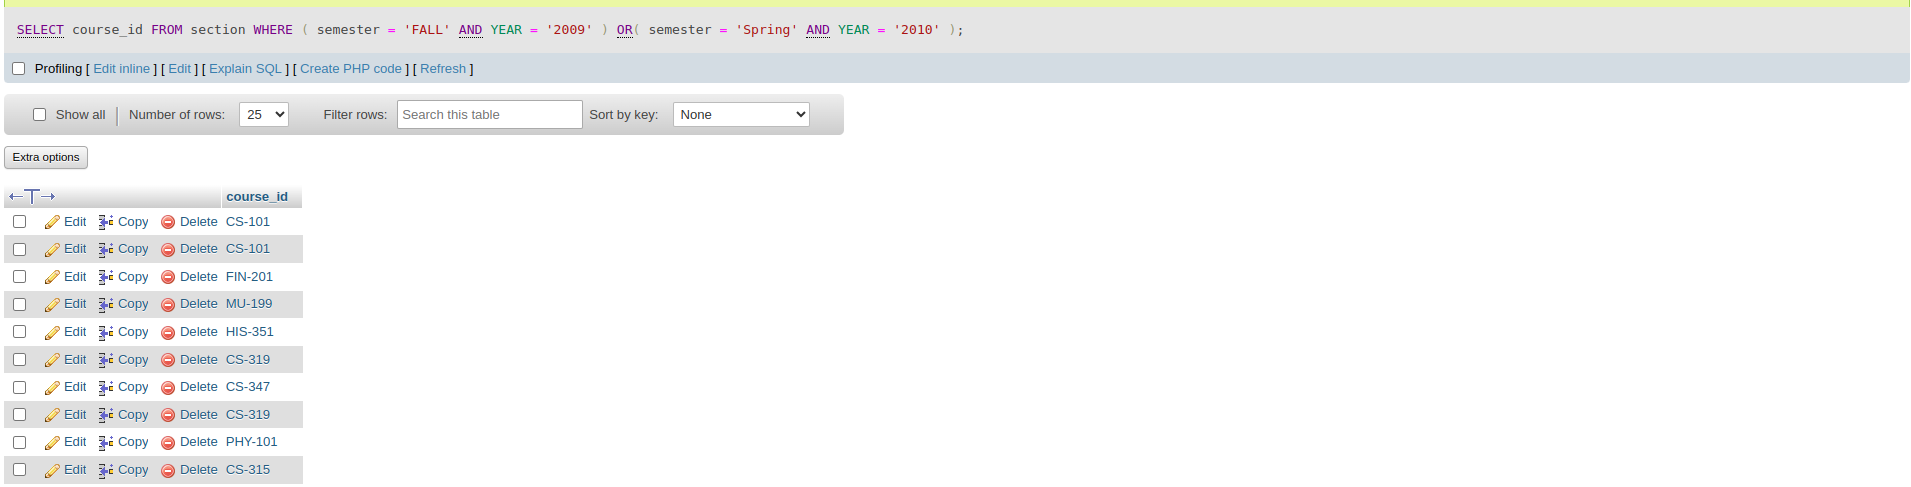
\includegraphics[width=1.0\textwidth]{fig/43.png}
\end{figure}

\begin{verbatim}
(SELECT course_id 
FROM section 
WHERE semester = 'FALL' AND year = '2009')
INTERSECT
(SELECT course_id 
FROM section 
WHERE semester = 'Spring' AND year = '2010');
\end{verbatim}
\begin{figure}[H]
    \centering
    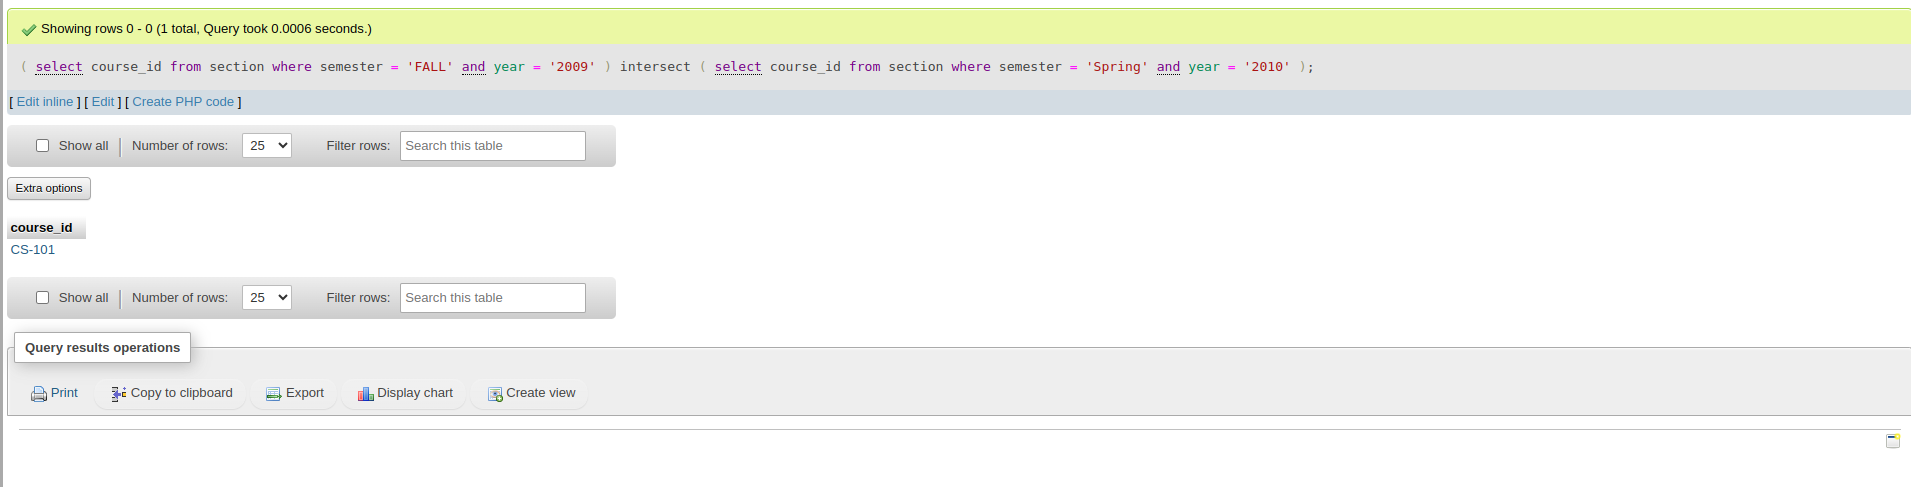
\includegraphics[width=1.0\textwidth]{fig/44.png}
\end{figure}

\begin{verbatim}
(SELECT course_id 
FROM section 
WHERE semester = 'FALL' AND year = '2009')
EXCEPT
(SELECT course_id 
FROM section 
WHERE semester = 'Spring' AND year = '2010');
\end{verbatim}
\begin{figure}[H]
    \centering
    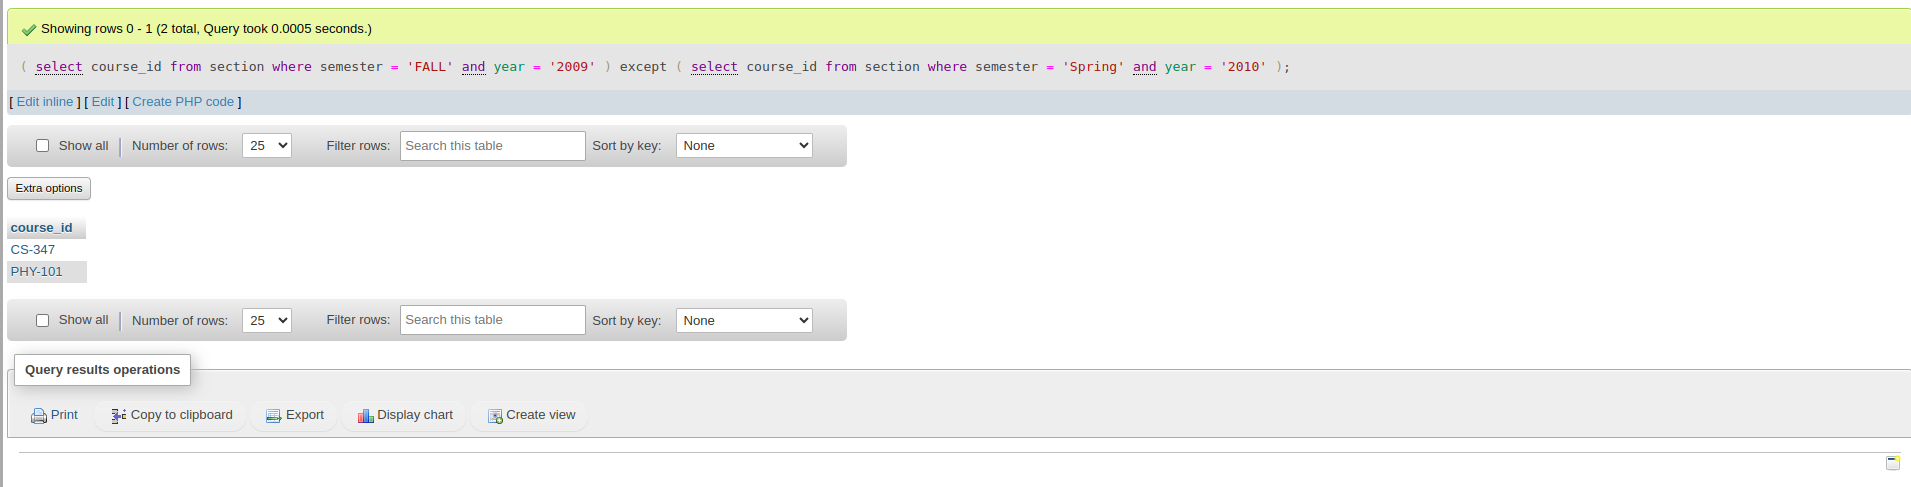
\includegraphics[width=1.0\textwidth]{fig/45.png}
\end{figure}

\begin{verbatim}
SELECT ID, name, dept_name, salary / 12 
FROM instructor;
\end{verbatim}
\begin{figure}[H]
    \centering
    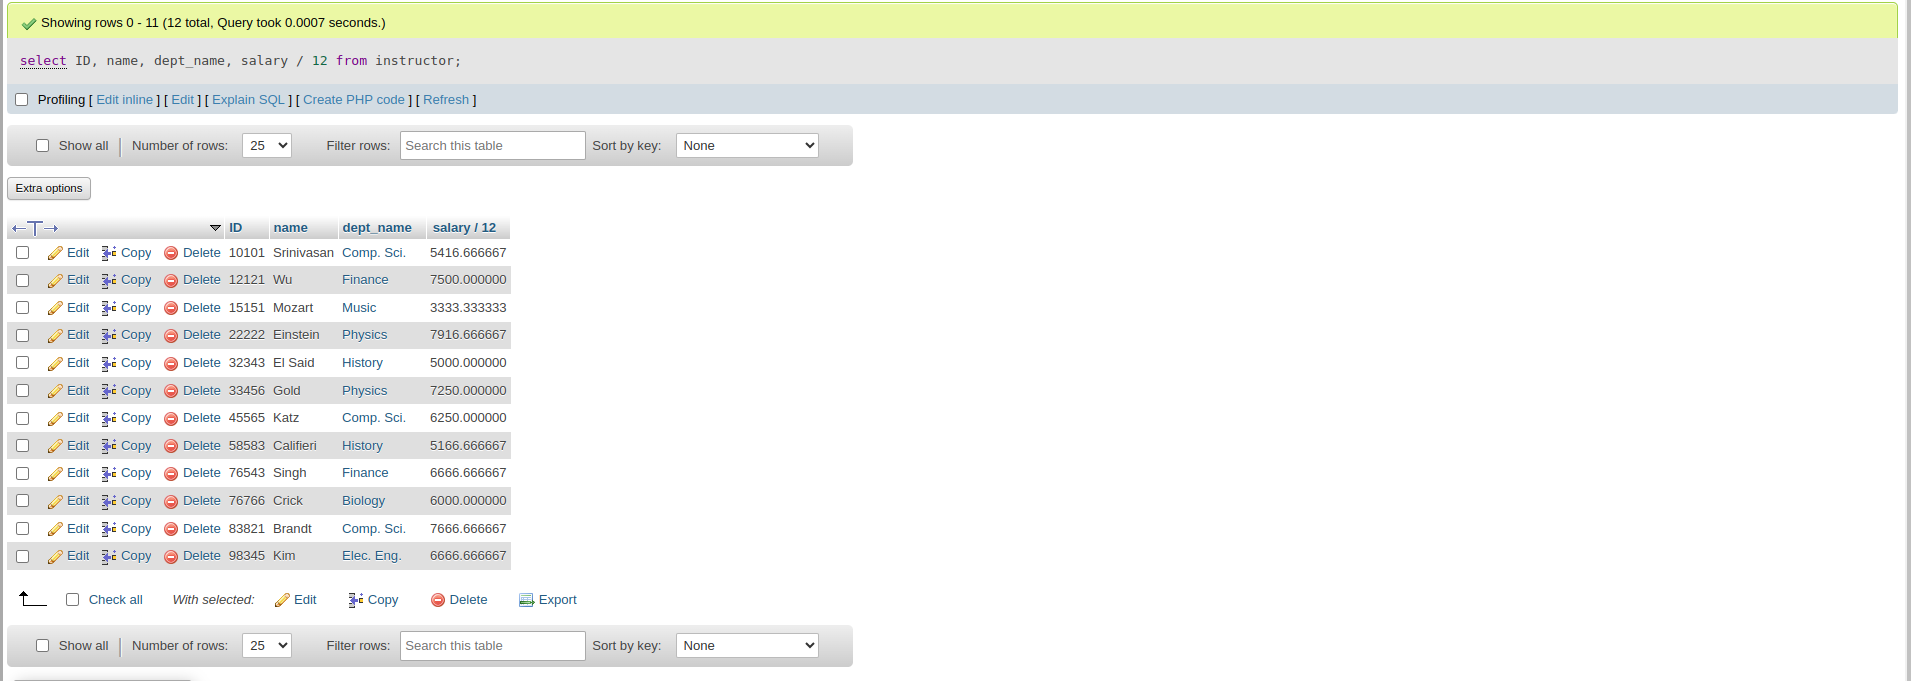
\includegraphics[width=1.0\textwidth]{fig/46.png}
\end{figure}

\begin{verbatim}
SELECT name, course_id 
FROM instructor, teaches 
WHERE instructor.ID = teaches.ID AND dept_name = 'Biology';
\end{verbatim}
\begin{figure}[H]
    \centering
    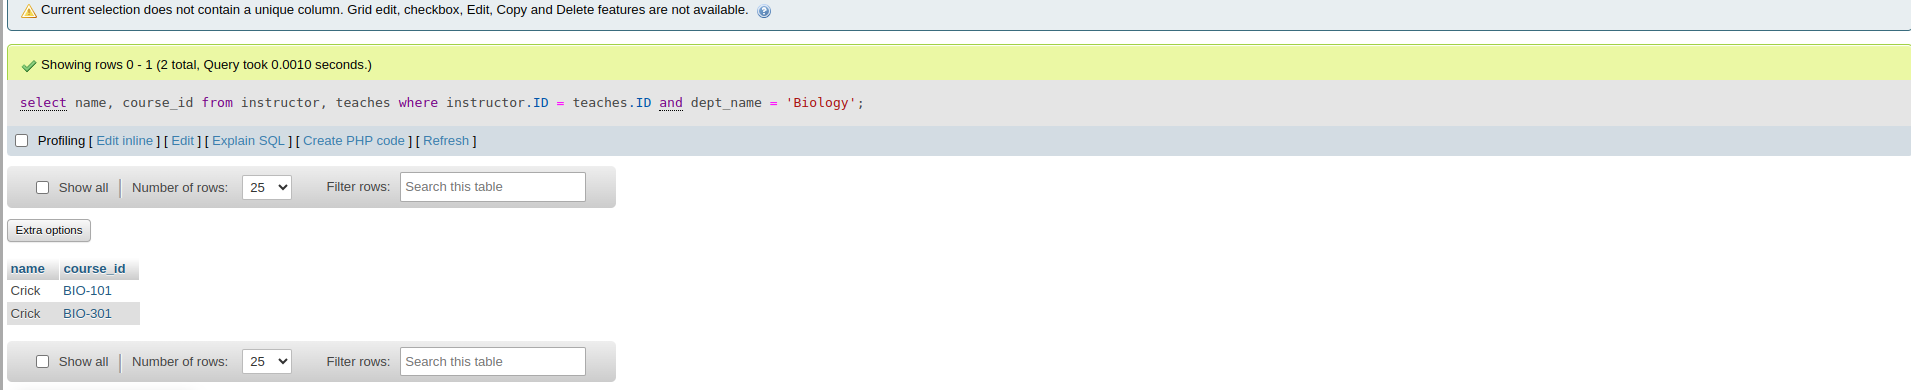
\includegraphics[width=1.0\textwidth]{fig/47.png}
\end{figure}

\begin{verbatim}
SELECT NAME, course_id 
FROM instructor AS I, teaches AS T 
WHERE I.ID = T.ID AND dept_name = 'Biology';
\end{verbatim}
\begin{figure}[H]
    \centering
    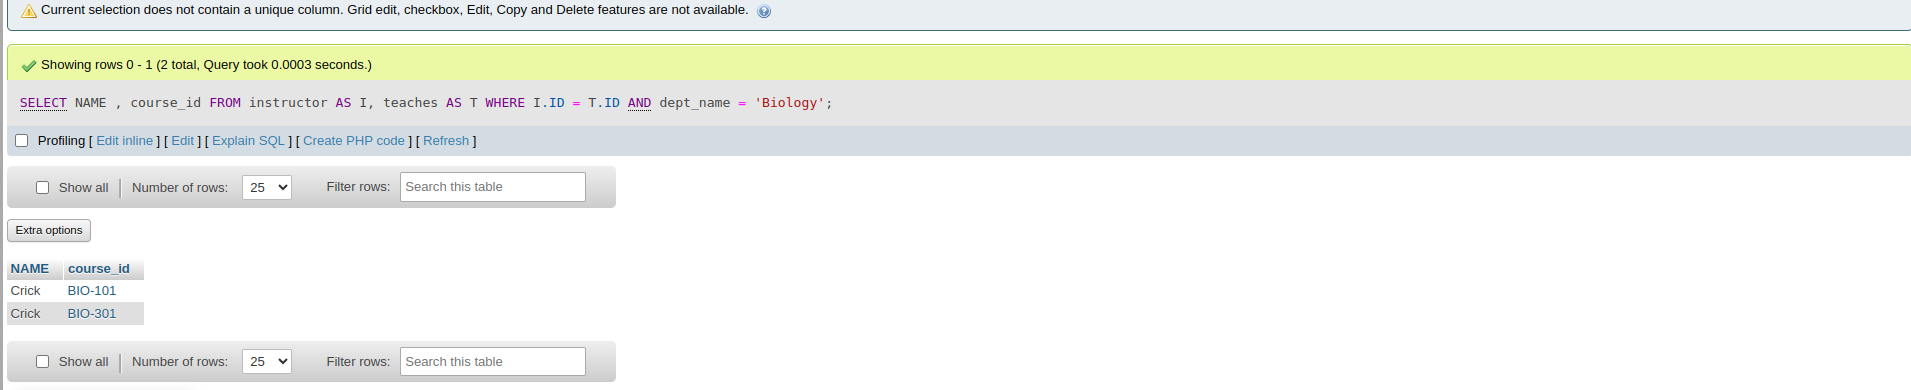
\includegraphics[width=1.0\textwidth]{fig/48.png}
\end{figure}

\begin{verbatim}
SELECT DISTINCT T.salary 
FROM instructor AS T, instructor AS S 
WHERE T.salary < S.salary AND S.dept_name = 'Biology';
\end{verbatim}
\begin{figure}[H]
    \centering
    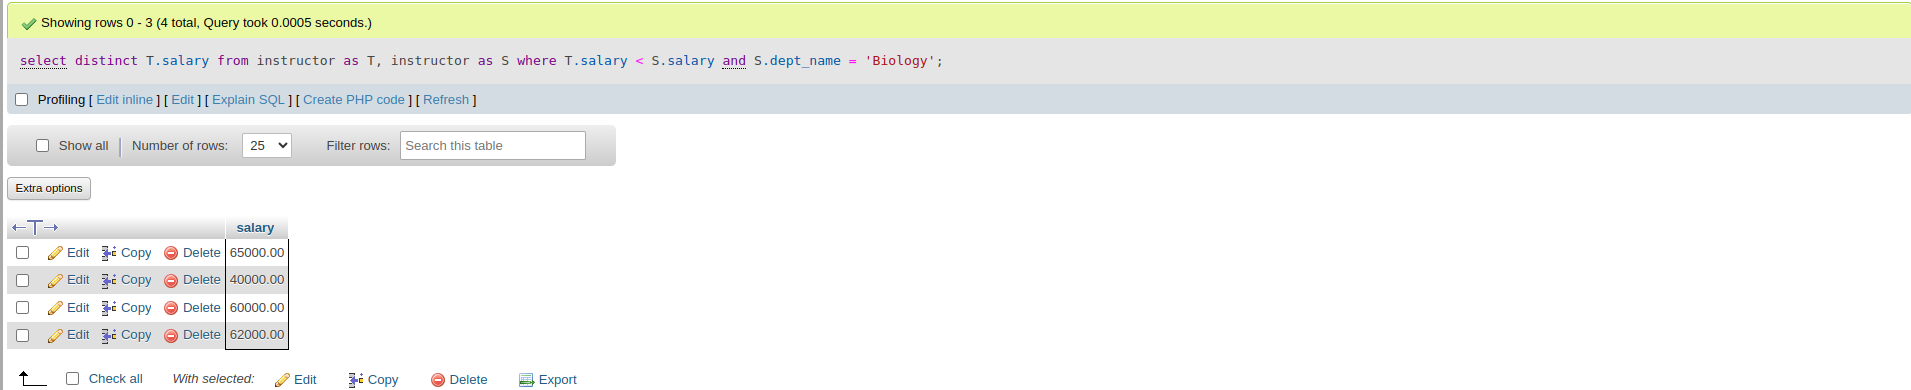
\includegraphics[width=1.0\textwidth]{fig/49.png}
\end{figure}

\begin{verbatim}
SELECT * 
FROM instructor, teaches;
\end{verbatim}
\begin{figure}[H]
    \centering
    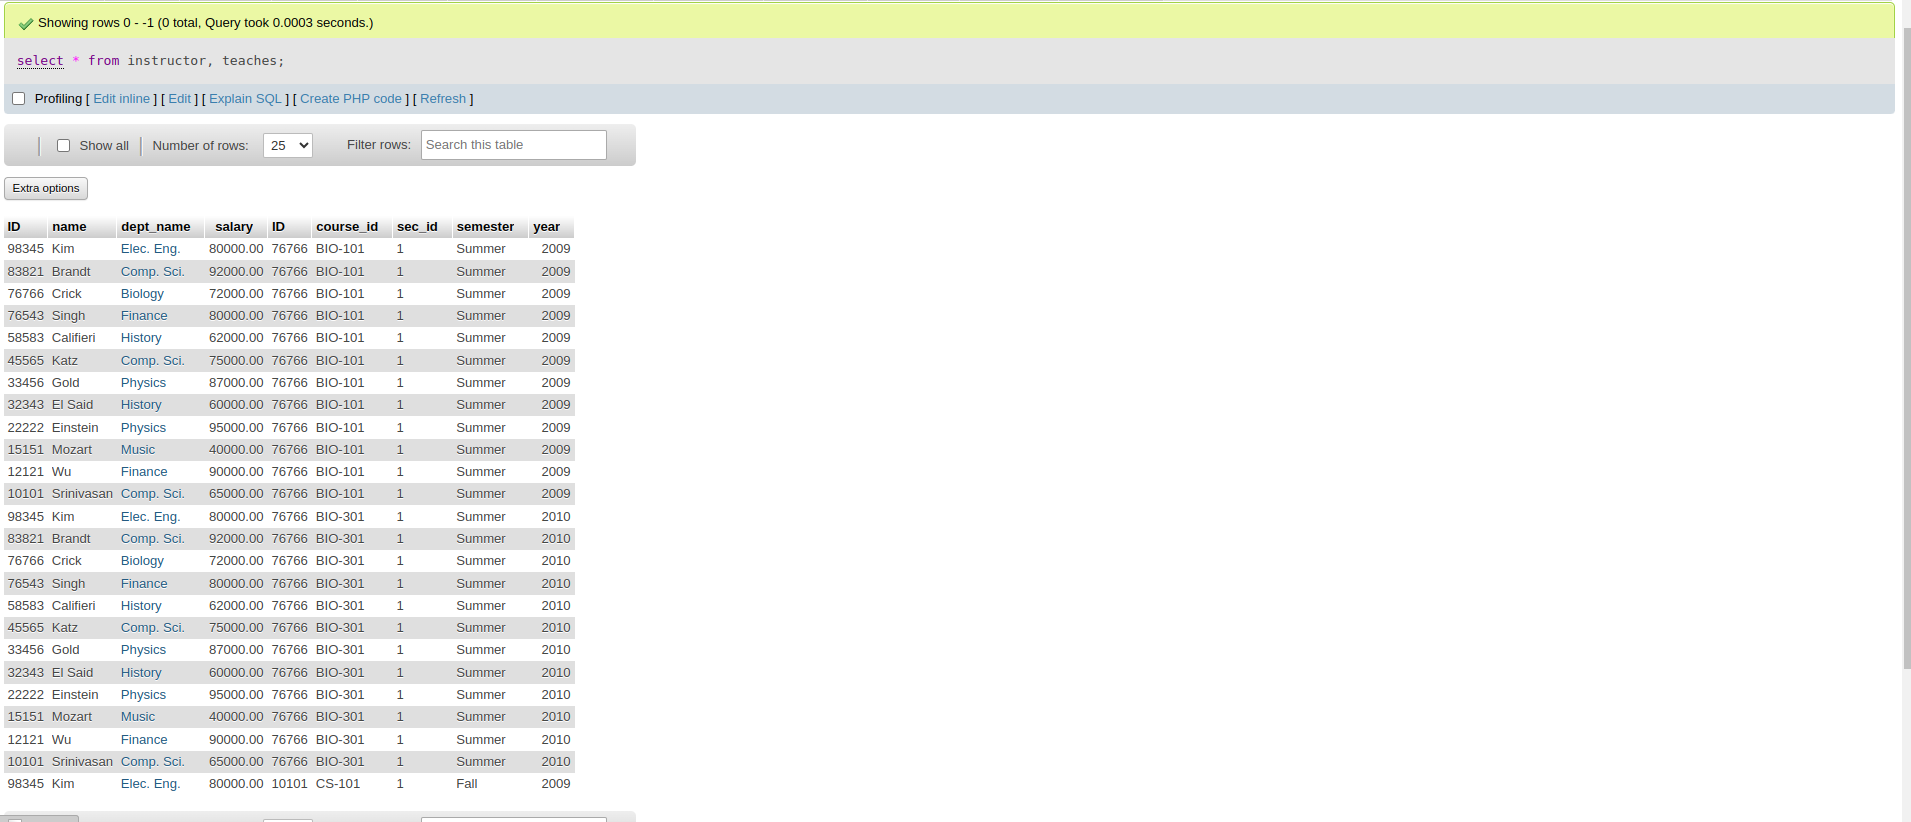
\includegraphics[width=1.0\textwidth]{fig/50.png}
\end{figure}

\begin{verbatim}
SELECT DISTINCT name 
FROM instructor 
ORDER BY name;
\end{verbatim}
\begin{figure}[H]
    \centering
    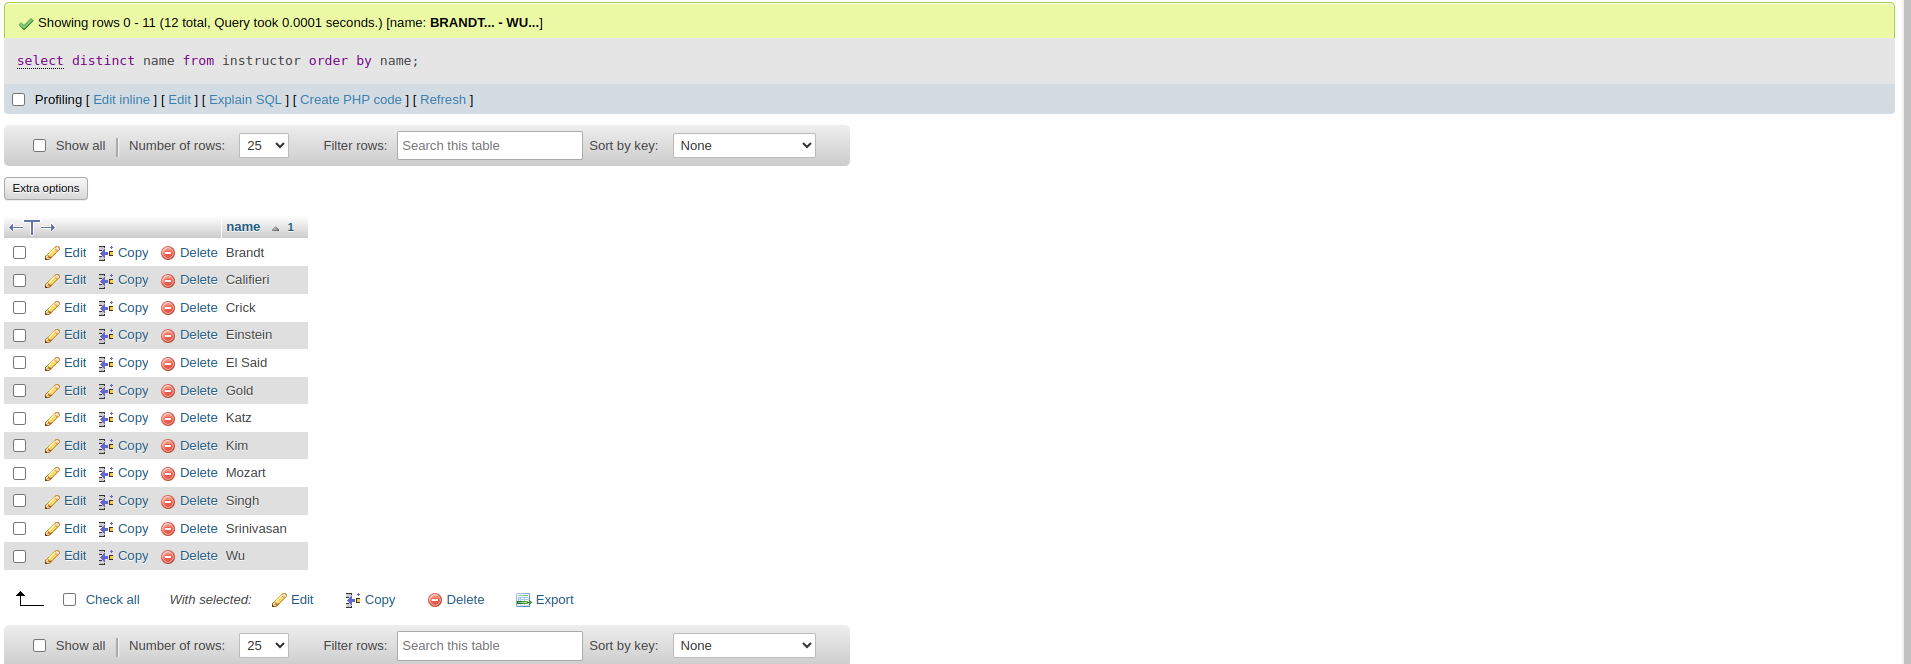
\includegraphics[width=1.0\textwidth]{fig/51.png}
\end{figure}

\begin{verbatim}
SELECT * 
FROM instructor 
ORDER BY salary DESC, name ASC;
\end{verbatim}
\begin{figure}[H]
    \centering
    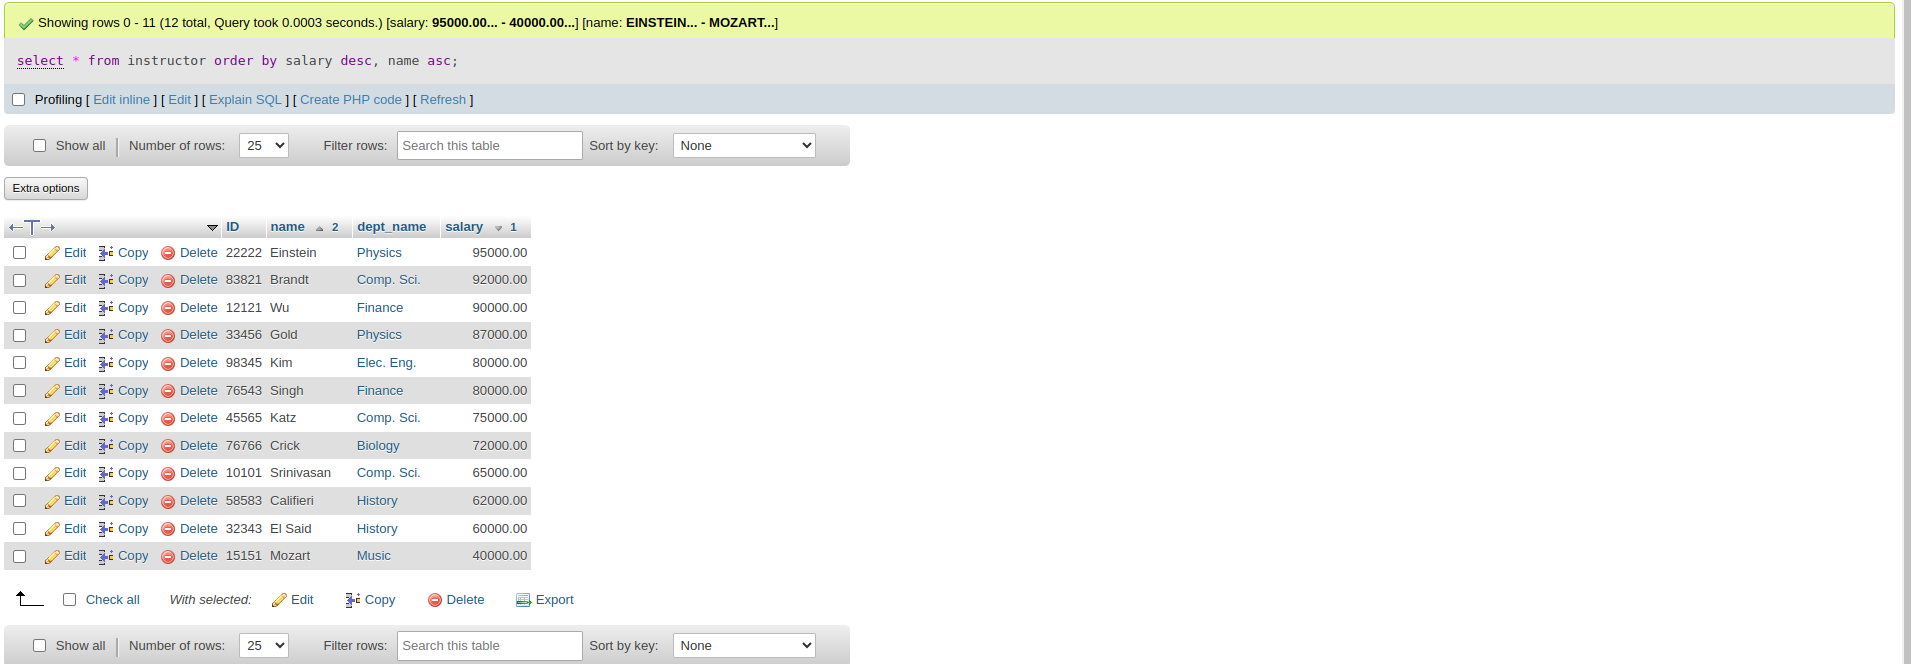
\includegraphics[width=1.0\textwidth]{fig/52.png}
\end{figure}
%%%%%%%%%%%%%%%%%%%%%%%%%%%%%%%%%%%%%%%%%%%%%%%%%%%%%%%%%%%%%%%%%%%%%%%%%%%%%%%%%%%%%%
%bahromiddin

\begin{verbatim}
SELECT name FROM instructor WHERE name LIKE '%dar%';
\end{verbatim}
\begin{figure}[H]
    \centering
    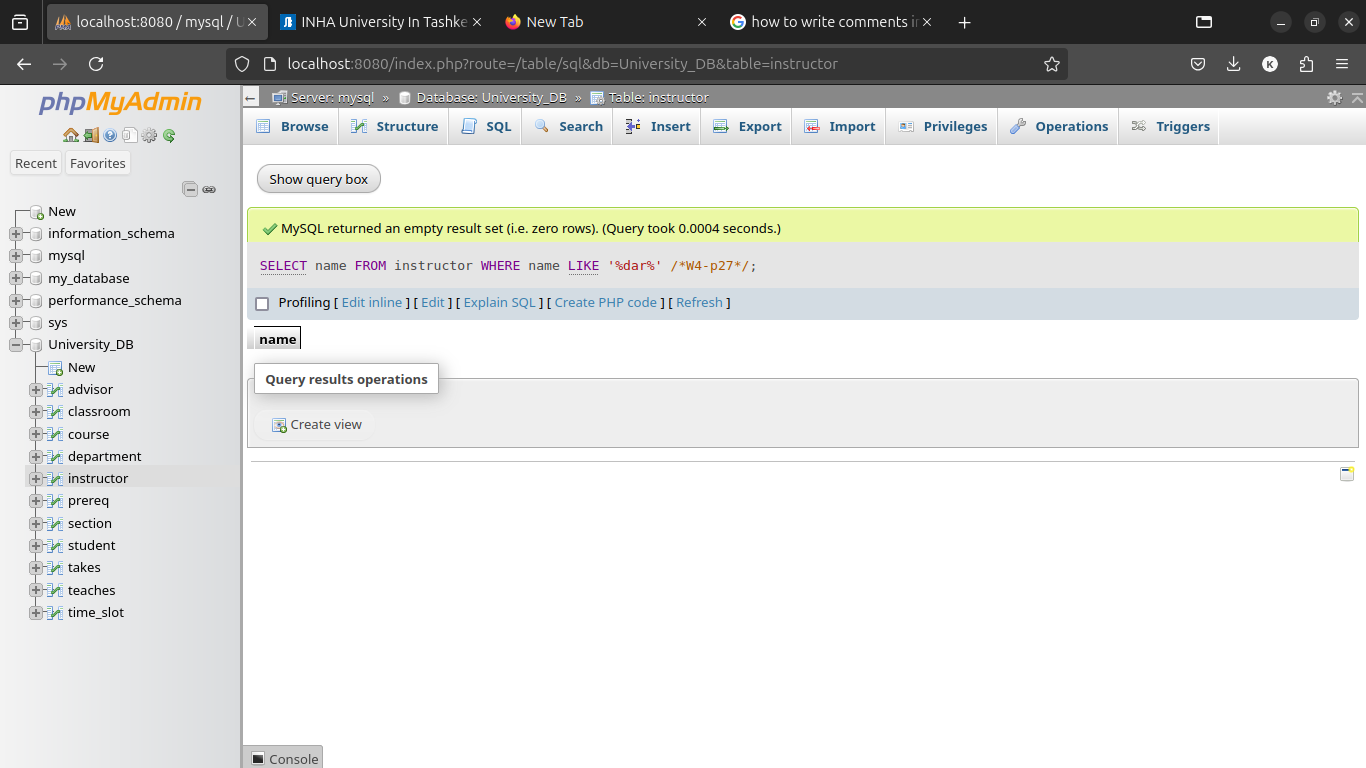
\includegraphics[width=1.0\textwidth]{fig/53.png}
\end{figure}

\begin{verbatim}
SELECT name FROM instructor WHERE salary BETWEEN 90000 AND 100000;
\end{verbatim}
\begin{figure}[H]
    \centering
    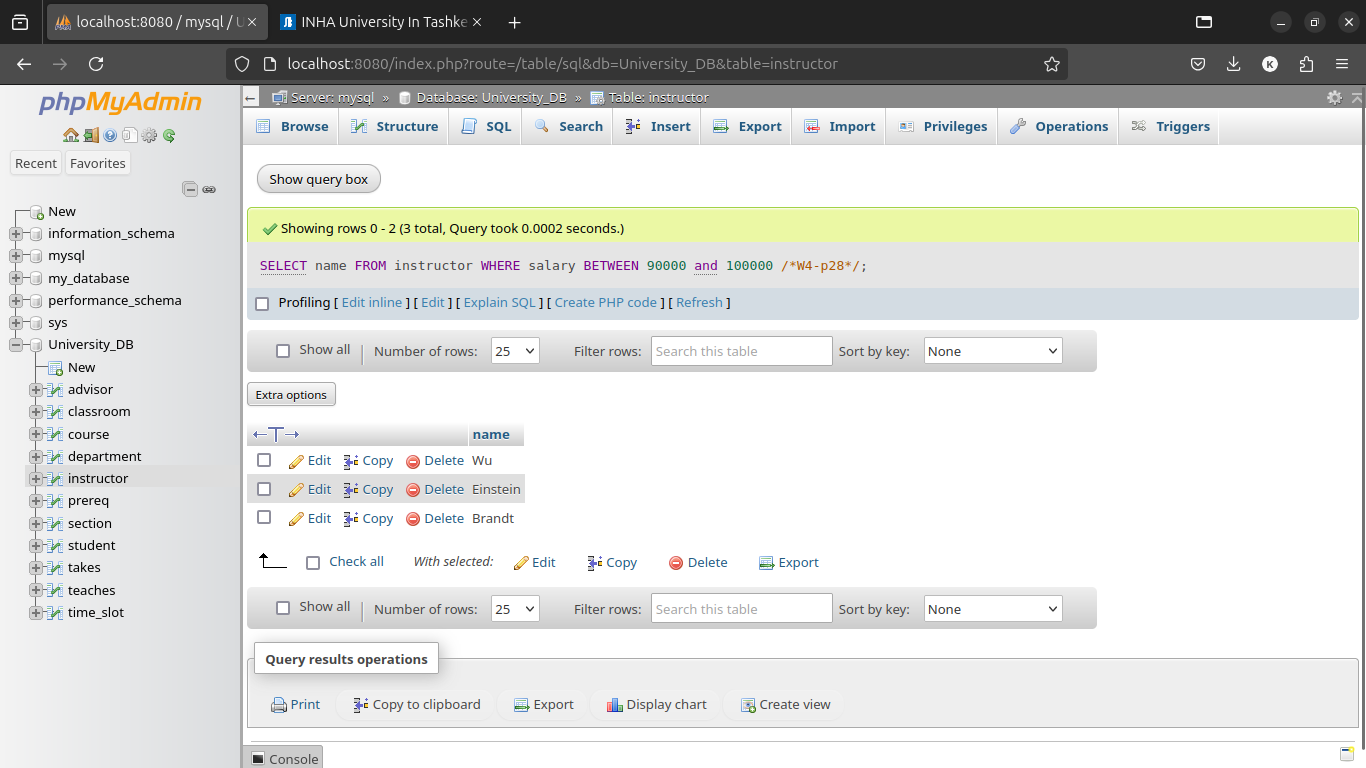
\includegraphics[width=1.0\textwidth]{fig/54.png}
\end{figure}

\begin{verbatim}
SELECT name, course_id 
FROM instructor, teaches 
WHERE instructor.ID = teaches.ID AND dept_name = 'Biology';
\end{verbatim}
\begin{figure}[H]
    \centering
    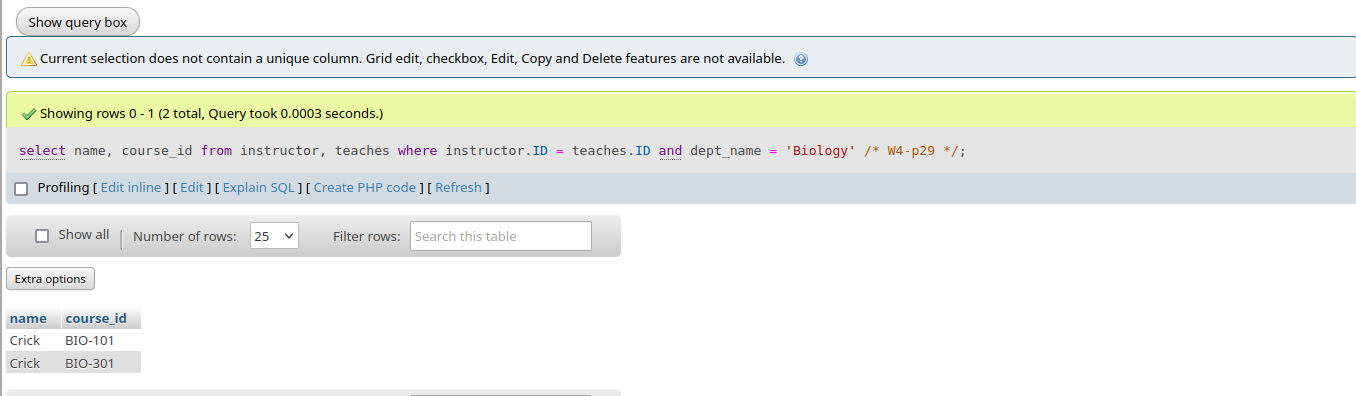
\includegraphics[width=1.0\textwidth]{fig/55.png}
\end{figure}

\begin{verbatim}
SELECT name, course_id 
FROM instructor, teaches 
WHERE (instructor.ID, dept_name) = (teaches.ID, 'Biology');
\end{verbatim}
\begin{figure}[H]
    \centering
    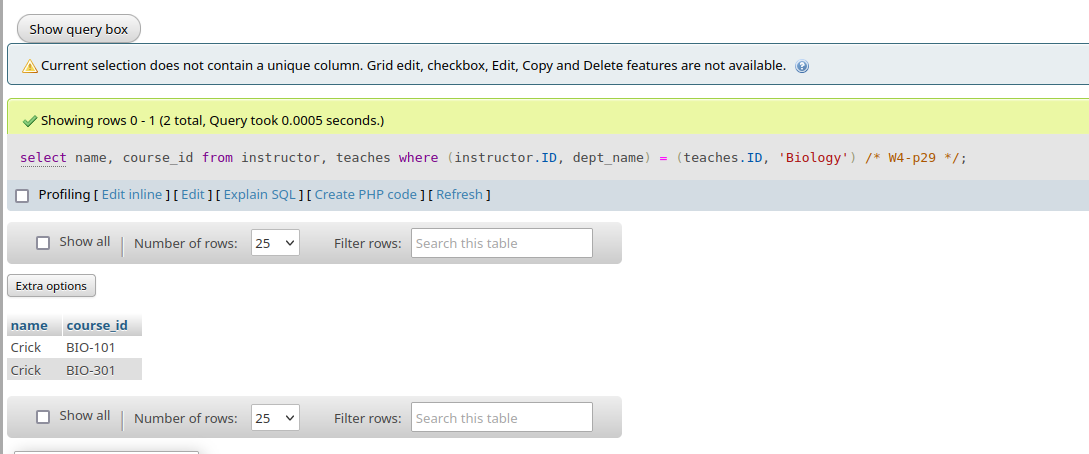
\includegraphics[width=1.0\textwidth]{fig/56.png}
\end{figure}

\begin{verbatim}
SELECT name FROM instructor WHERE salary IS NULL;
\end{verbatim}
\begin{figure}[H]
    \centering
    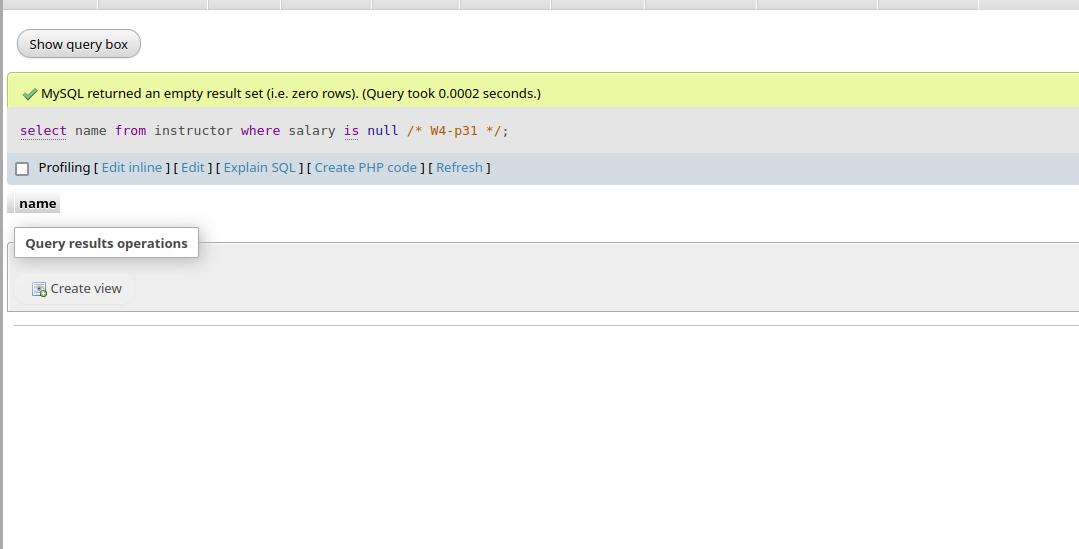
\includegraphics[width=1.0\textwidth]{fig/57.png}
\end{figure}

\begin{verbatim}
SELECT avg(salary) AS avg_salary 
FROM instructor 
WHERE dept_name = 'Comp. Sci.';
\end{verbatim}
\begin{figure}[H]
    \centering
    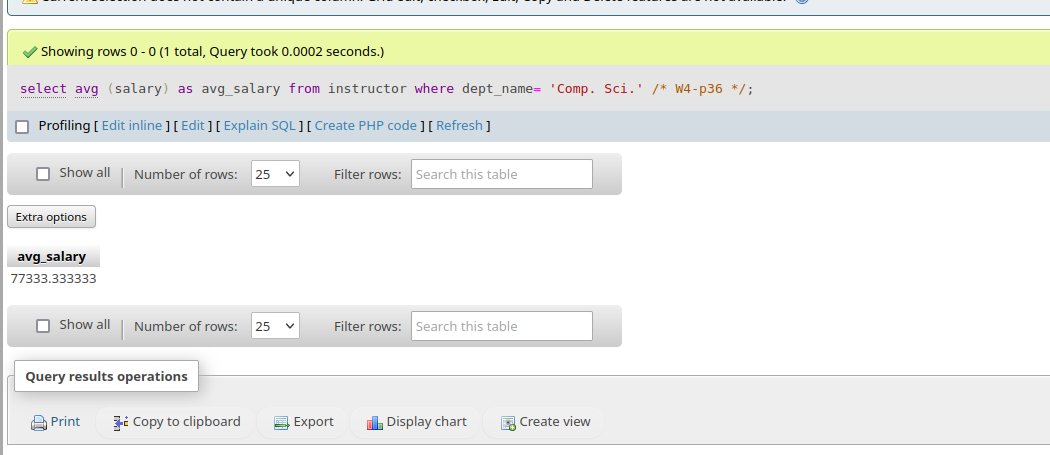
\includegraphics[width=1.0\textwidth]{fig/58.png}
\end{figure}

\begin{verbatim}
SELECT avg(salary) AS avg_salary 
FROM instructor 
WHERE dept_name = 'Comp. Sci.';
\end{verbatim}
\begin{figure}[H]
    \centering
    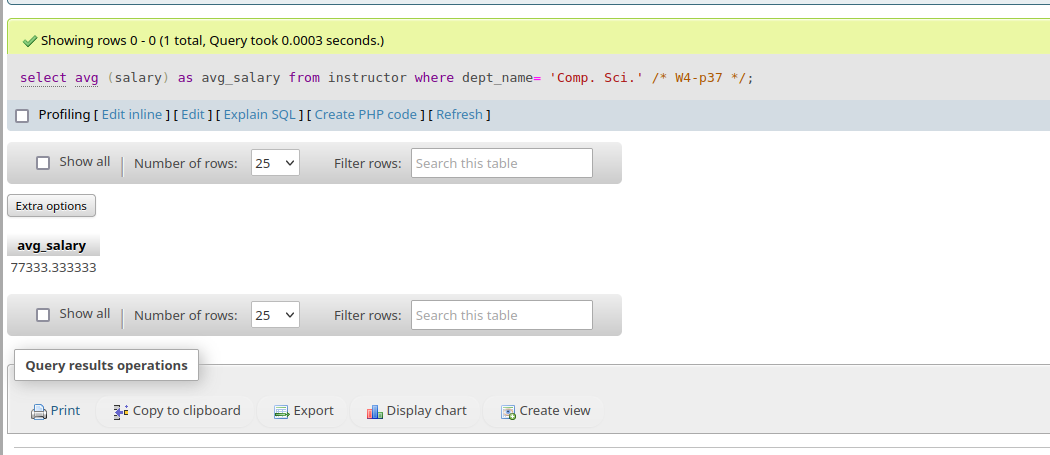
\includegraphics[width=1.0\textwidth]{fig/59.png}
\end{figure}

\begin{verbatim}
SELECT count(DISTINCT ID) 
FROM teaches 
WHERE semester = 'Spring' AND year = 2010;
\end{verbatim}
\begin{figure}[H]
    \centering
    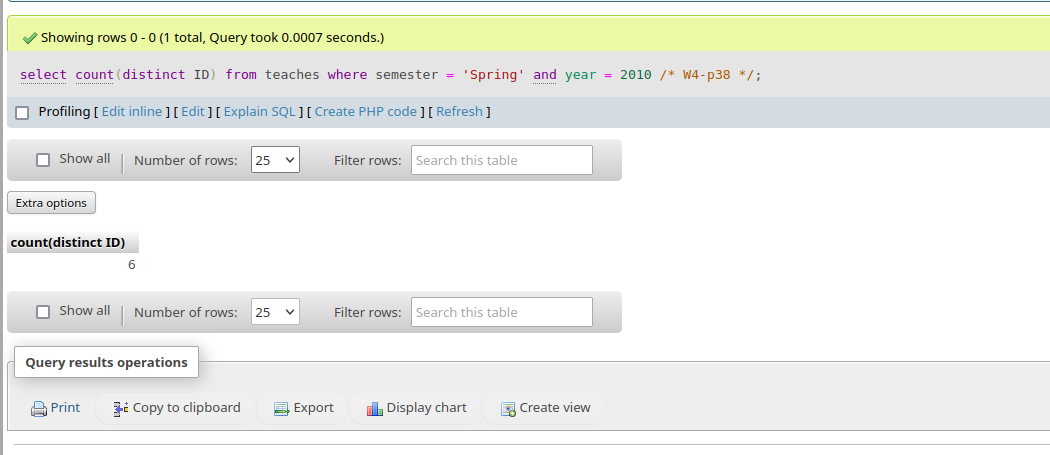
\includegraphics[width=1.0\textwidth]{fig/60.png}
\end{figure}

\begin{verbatim}
SELECT count(*) 
FROM course;
\end{verbatim}
\begin{figure}[H]
    \centering
    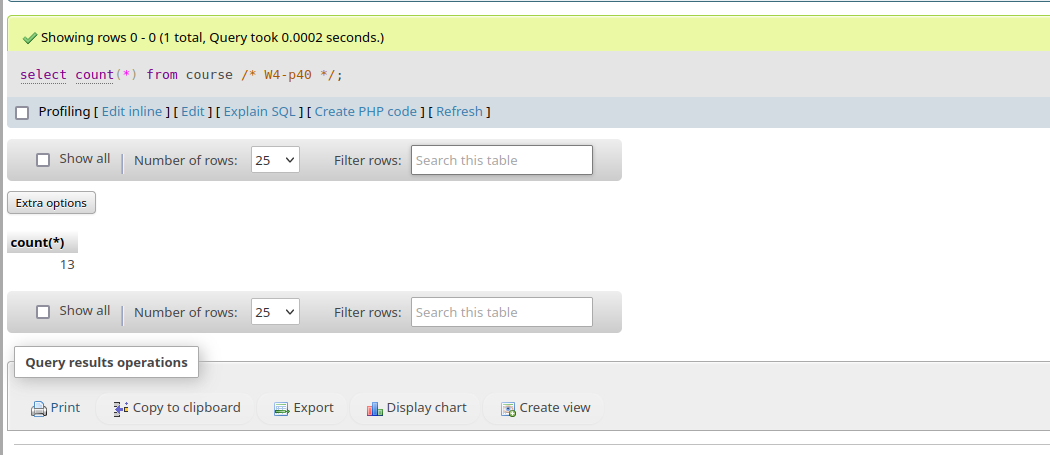
\includegraphics[width=1.0\textwidth]{fig/61.png}
\end{figure}

\begin{verbatim}
SELECT dept_name, avg(salary) AS avg_salary 
FROM instructor 
GROUP BY dept_name;
\end{verbatim}
\begin{figure}[H]
    \centering
    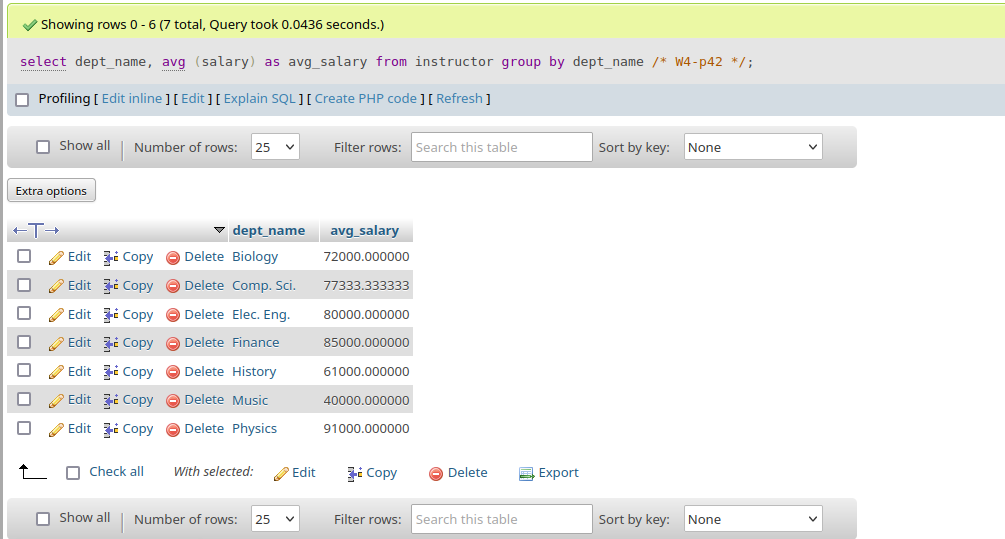
\includegraphics[width=1.0\textwidth]{fig/62.png}
\end{figure}

\begin{verbatim}
SELECT dept_name, ID, avg(salary) AS avg_salary 
FROM instructor 
GROUP BY dept_name, ID;
\end{verbatim}
\begin{figure}[H]
    \centering
    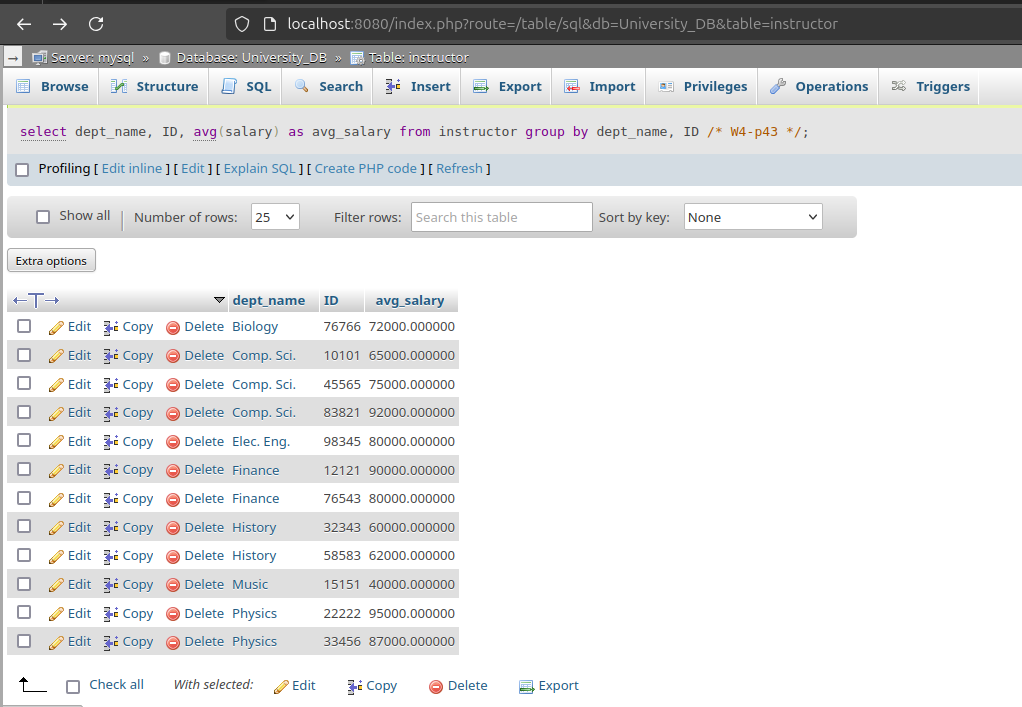
\includegraphics[width=1.0\textwidth]{fig/63.png}
\end{figure}

\begin{verbatim}
SELECT avg(salary) AS avg_salary 
FROM instructor;
\end{verbatim}
\begin{figure}[H]
    \centering
    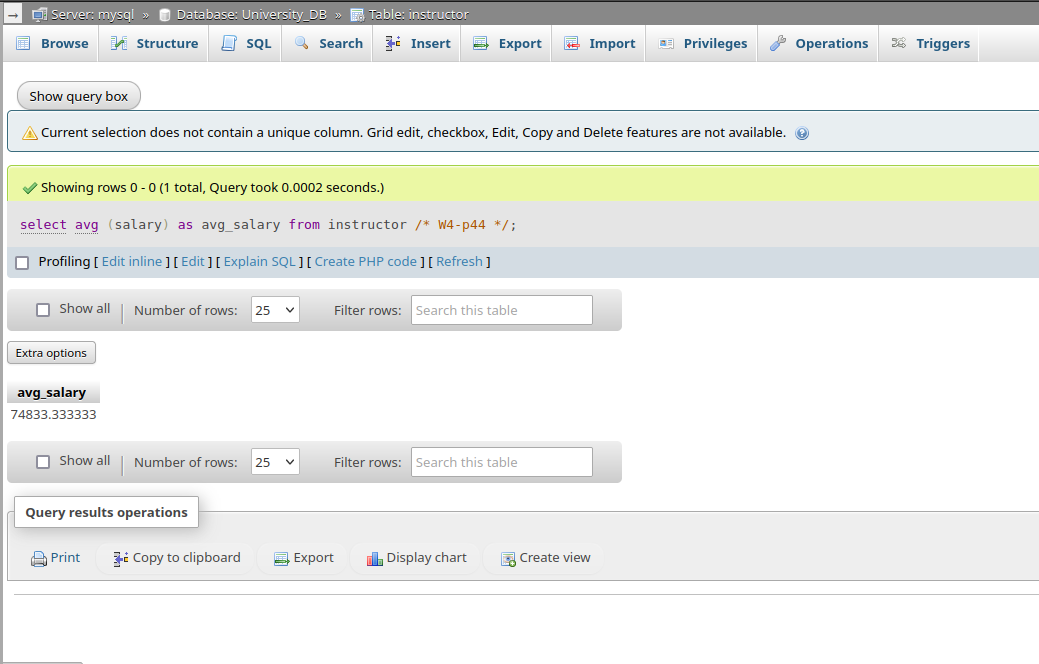
\includegraphics[width=1.0\textwidth]{fig/64.png}
\end{figure}

\begin{verbatim}
SELECT dept_name, count(DISTINCT ID) AS instr_count 
FROM instructor NATURAL JOIN teaches 
WHERE semester = 'Spring' AND year = 2010 
GROUP BY dept_name;
\end{verbatim}
\begin{figure}[H]
    \centering
    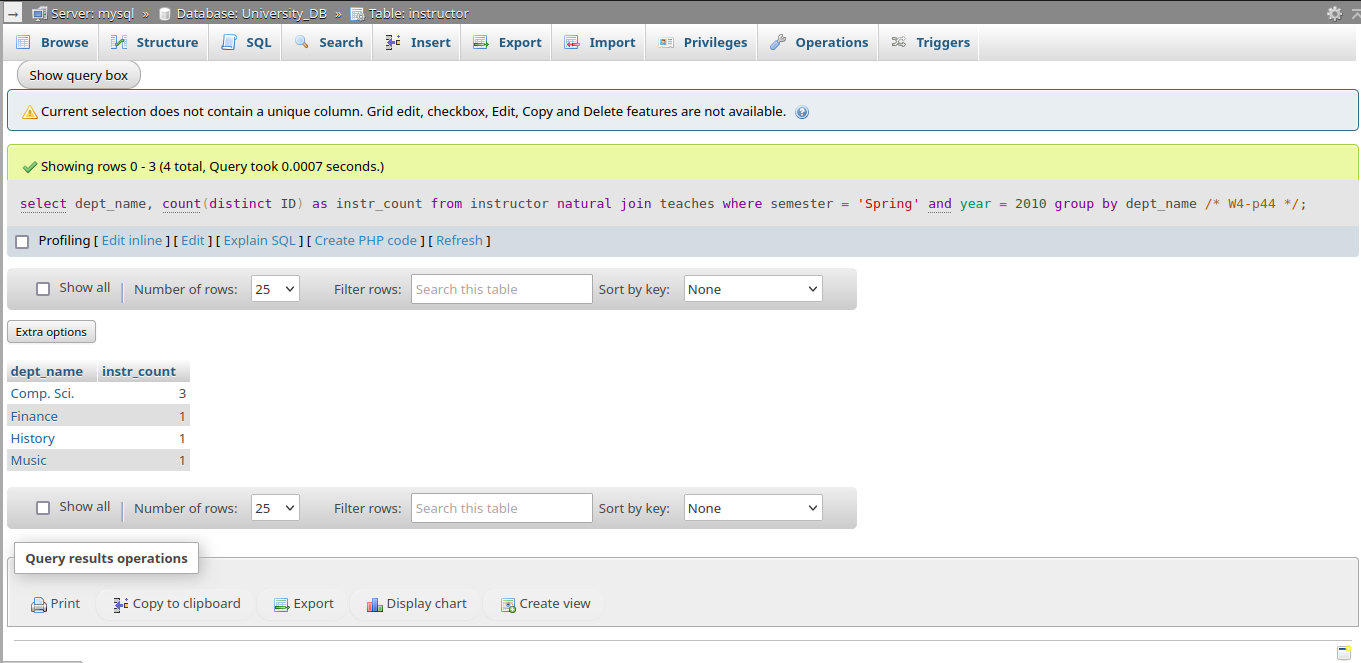
\includegraphics[width=1.0\textwidth]{fig/65.png}
\end{figure}

\begin{verbatim}
SELECT dept_name, avg(salary) AS avg_salary 
FROM instructor 
GROUP BY dept_name 
HAVING avg(salary) > 42000;
\end{verbatim}
\begin{figure}[H]
    \centering
    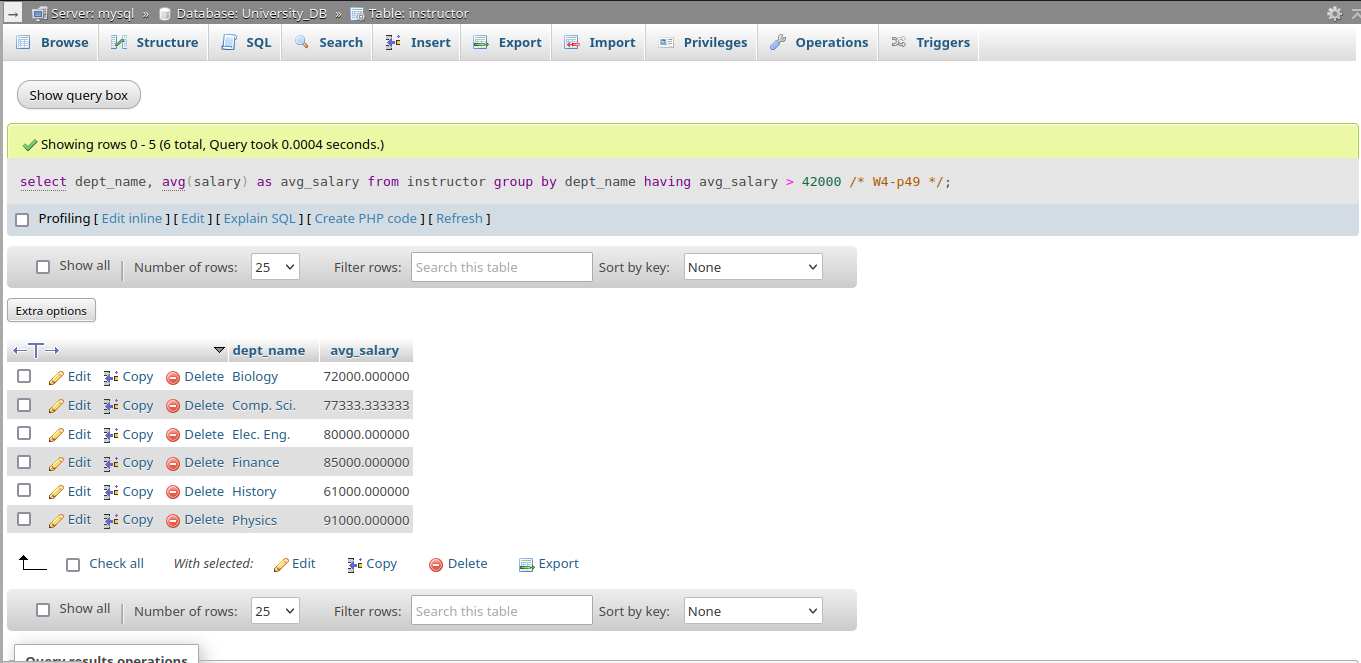
\includegraphics[width=1.0\textwidth]{fig/66.png}
\end{figure}

\begin{verbatim}
SELECT course_id, semester, year, sec_id, avg(tot_cred) AS avg_tot_cred 
FROM takes NATURAL JOIN student 
WHERE year = 2009 
GROUP BY course_id, semester, year, sec_id 
HAVING count(ID) >= 2;
\end{verbatim}
\begin{figure}[H]
    \centering
    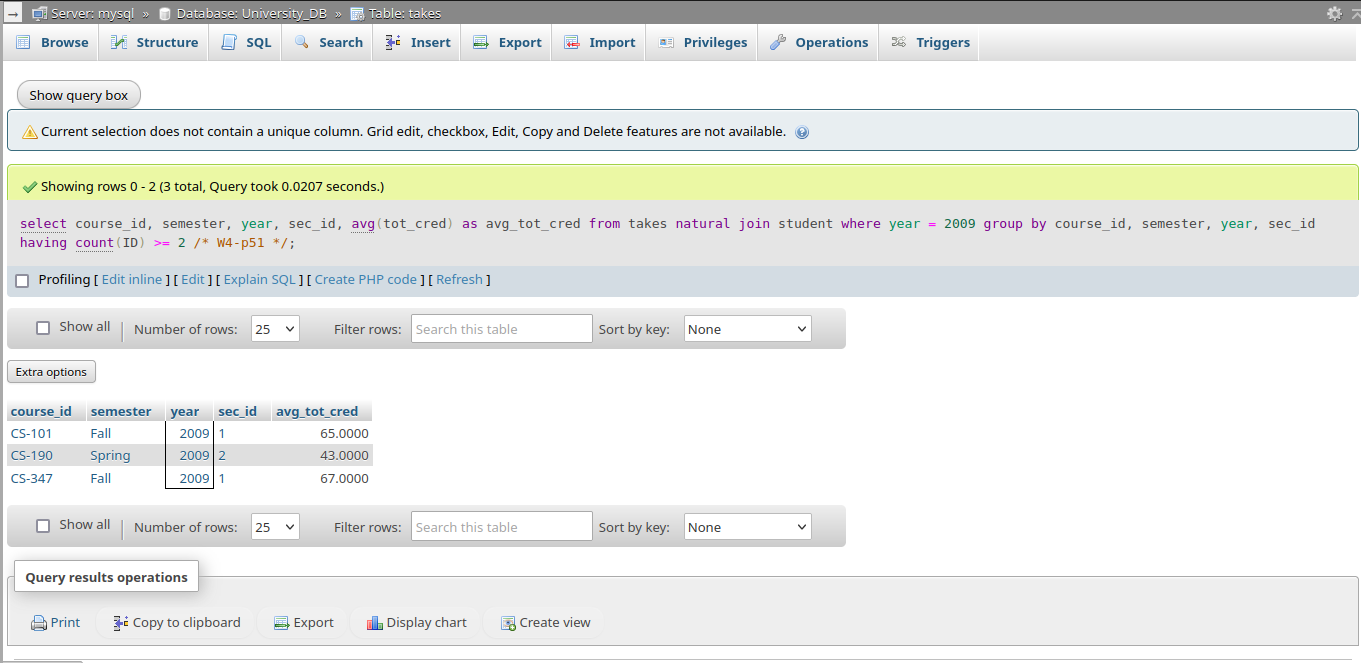
\includegraphics[width=1.0\textwidth]{fig/67.png}
\end{figure}

\begin{verbatim}
SELECT course_id 
FROM section 
WHERE semester = 'Fall' AND year = '2009'
INTERSECT
SELECT course_id 
FROM section 
WHERE semester = 'Spring' AND year = '2010';
\end{verbatim}
\begin{figure}[H]
    \centering
    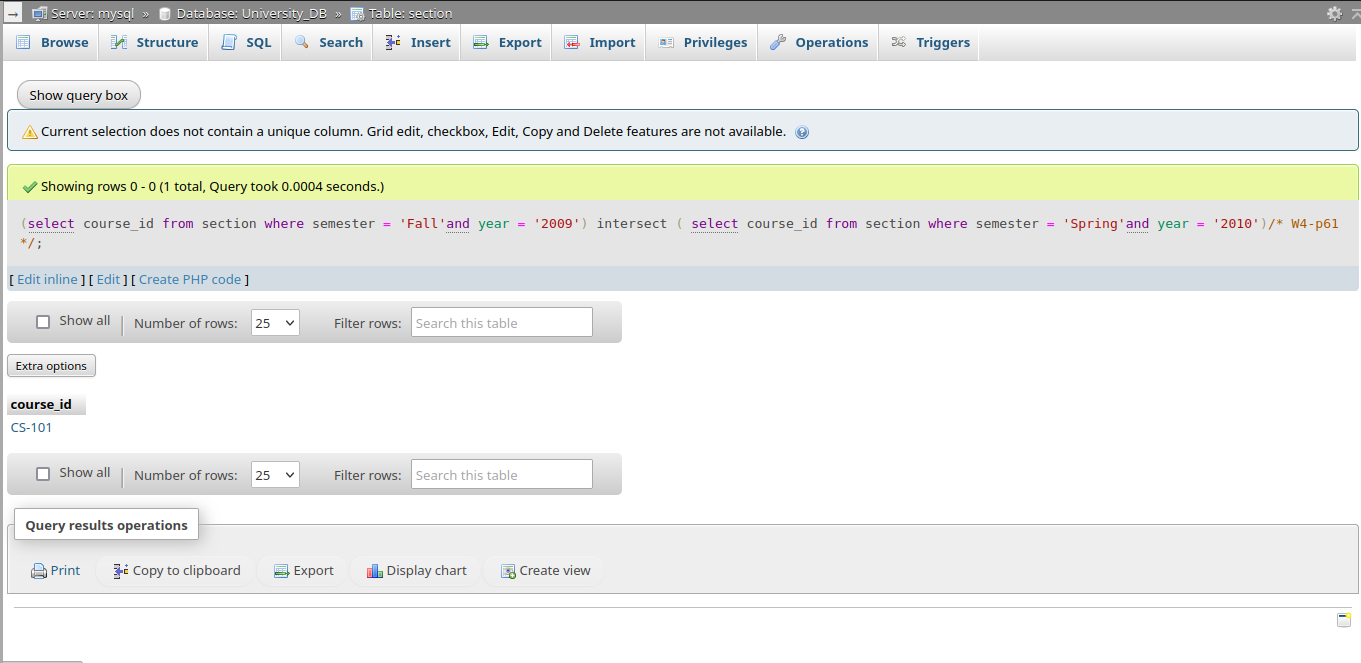
\includegraphics[width=1.0\textwidth]{fig/68.png}
\end{figure}

\begin{verbatim}
SELECT DISTINCT course_id 
FROM section AS S 
WHERE semester = 'Fall' AND year = 2009 
AND course_id IN (
    SELECT course_id 
    FROM section AS T 
    WHERE semester = 'Spring' AND year = 2010 
    AND T.course_id = S.course_id
);
\end{verbatim}
\begin{figure}[H]
    \centering
    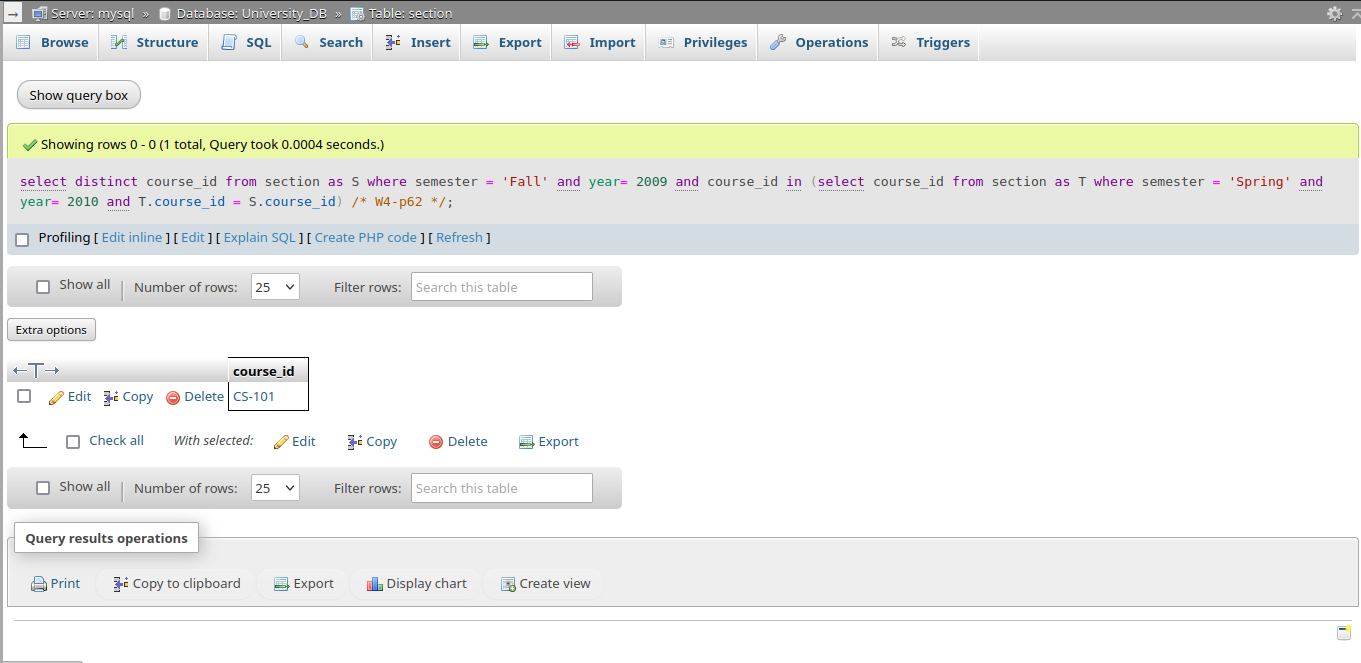
\includegraphics[width=1.0\textwidth]{fig/69.png}
\end{figure}

\begin{verbatim}
SELECT DISTINCT course_id 
FROM section 
WHERE semester = 'Fall' AND year = '2009'
EXCEPT
SELECT course_id 
FROM section 
WHERE semester = 'Spring' AND year = '2010';
\end{verbatim}
\begin{figure}[H]
    \centering
    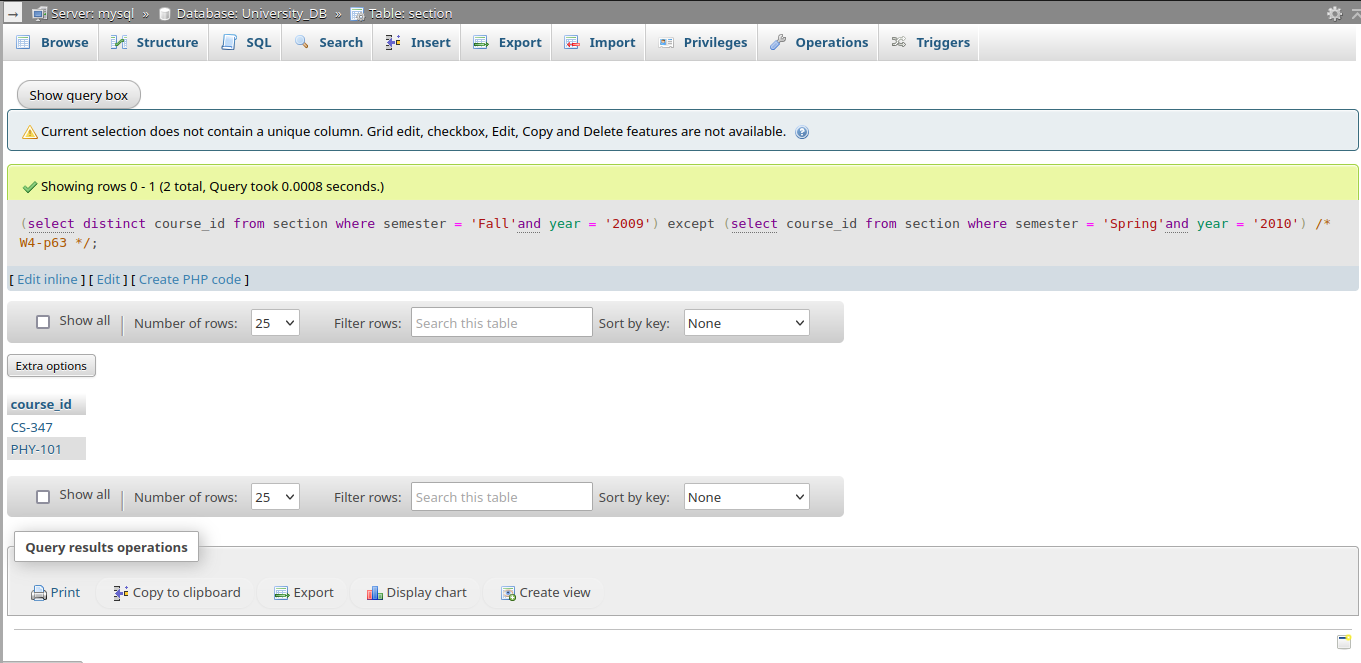
\includegraphics[width=1.0\textwidth]{fig/70.png}
\end{figure}

\begin{verbatim}
SELECT DISTINCT course_id 
FROM section 
WHERE semester = 'Fall' AND year = '2009' 
AND course_id NOT IN (
    SELECT course_id 
    FROM section 
    WHERE semester = 'Spring' AND year = 2010
);
\end{verbatim}
\begin{figure}[H]
    \centering
    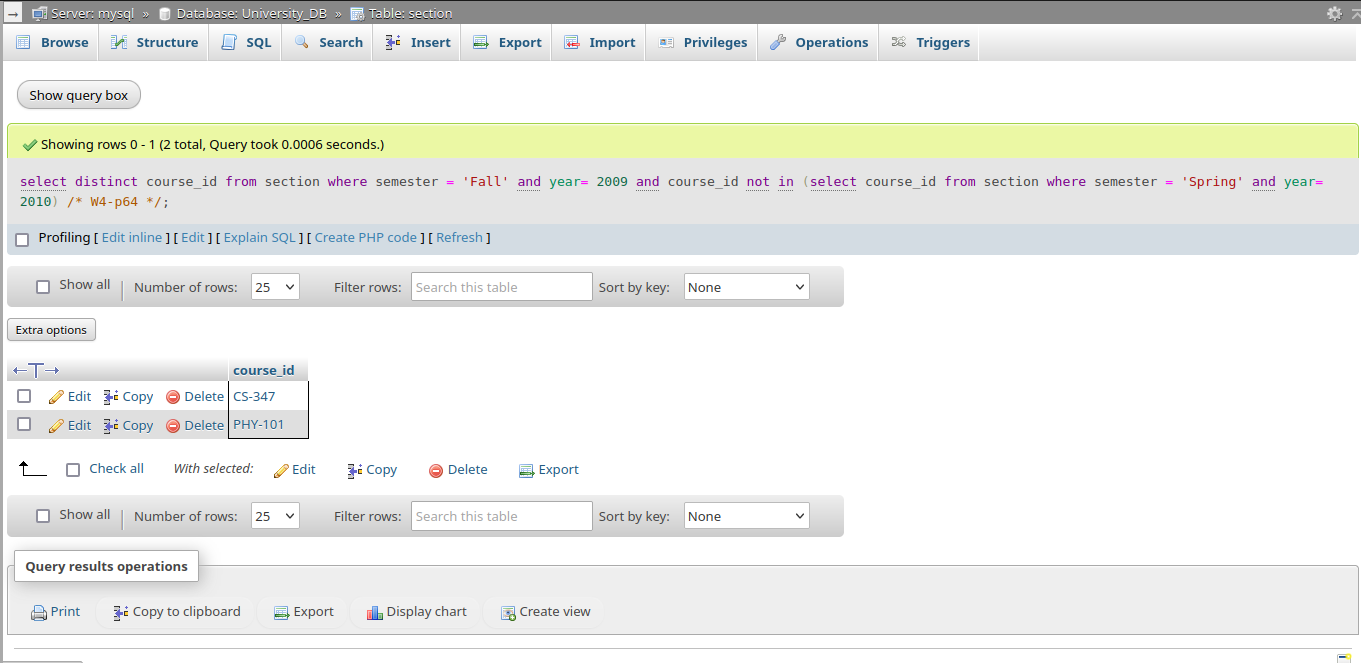
\includegraphics[width=1.0\textwidth]{fig/71.png}
\end{figure}

\begin{verbatim}
SELECT DISTINCT name 
FROM instructor 
WHERE name NOT IN ('Mozart', 'Einstein');
\end{verbatim}
\begin{figure}[H]
    \centering
    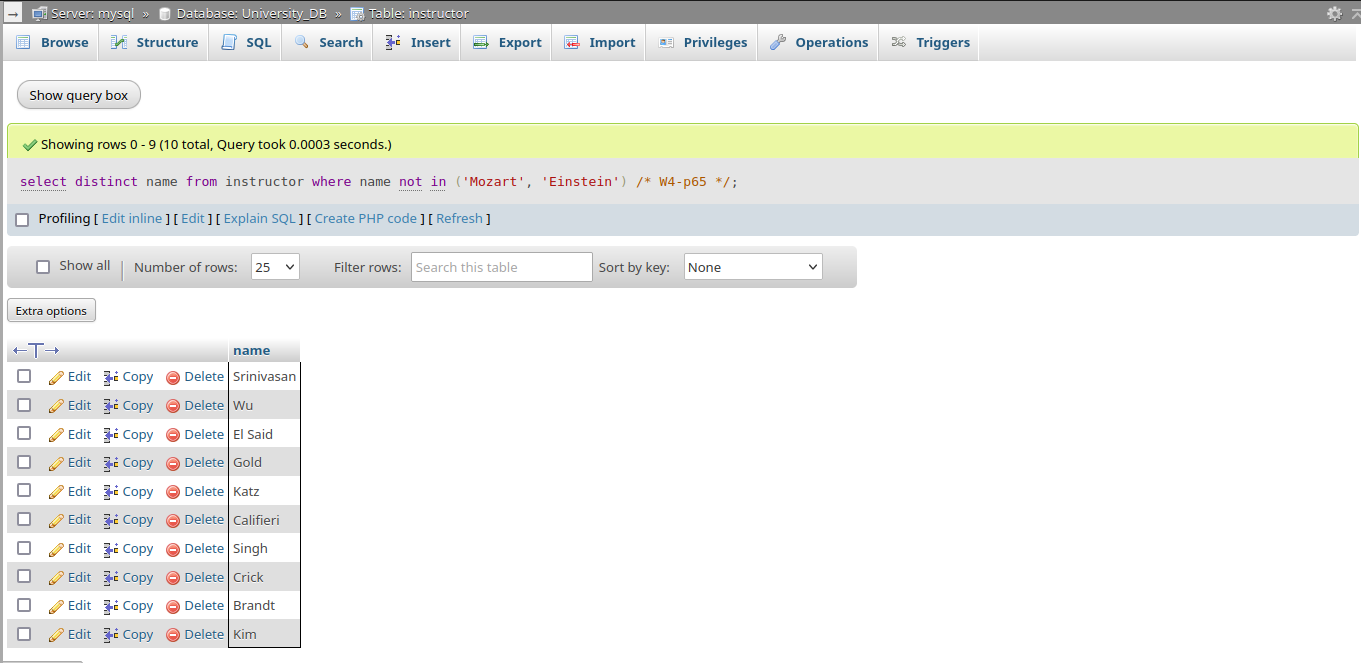
\includegraphics[width=1.0\textwidth]{fig/72.png}
\end{figure}
%%%%%%%%%%%%%%%%%%%%%%%%%%%%%%%%%%%%%%%%%%%%%%%%%%%%%%%%%%%%%%%%%%%%%%%%%%%%%%%%%%%%%%
%nargiza

\begin{verbatim}
73. SELECT COUNT(DISTINCT S.ID) FROM student as S, takes, section, teaches, instructor as I where I.ID='10101';
\end{verbatim}
\begin{figure}[h]
    \centering
    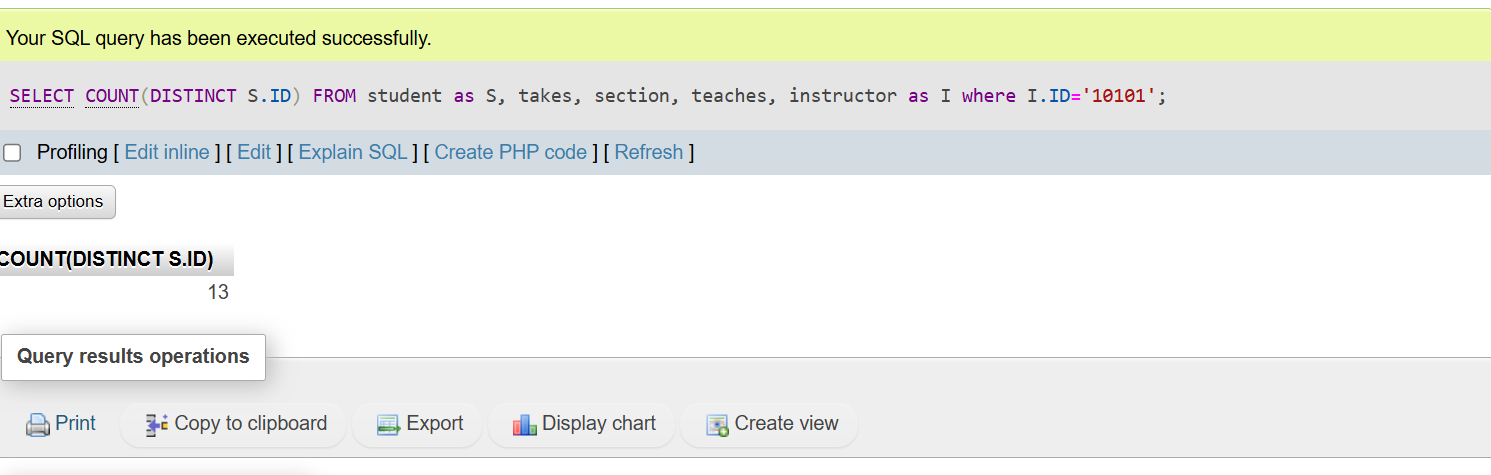
\includegraphics[width=1.0\textwidth]{fig/73.png}
    \caption{Query 73 Result}
\end{figure}

\begin{verbatim}
74. SELECT COUNT(DISTINCT S.ID) FROM takes AS S JOIN teaches AS I USING (course_id, sec_id, semester, year) WHERE I.ID = '10101';
\end{verbatim}
\begin{figure}[h]
    \centering
    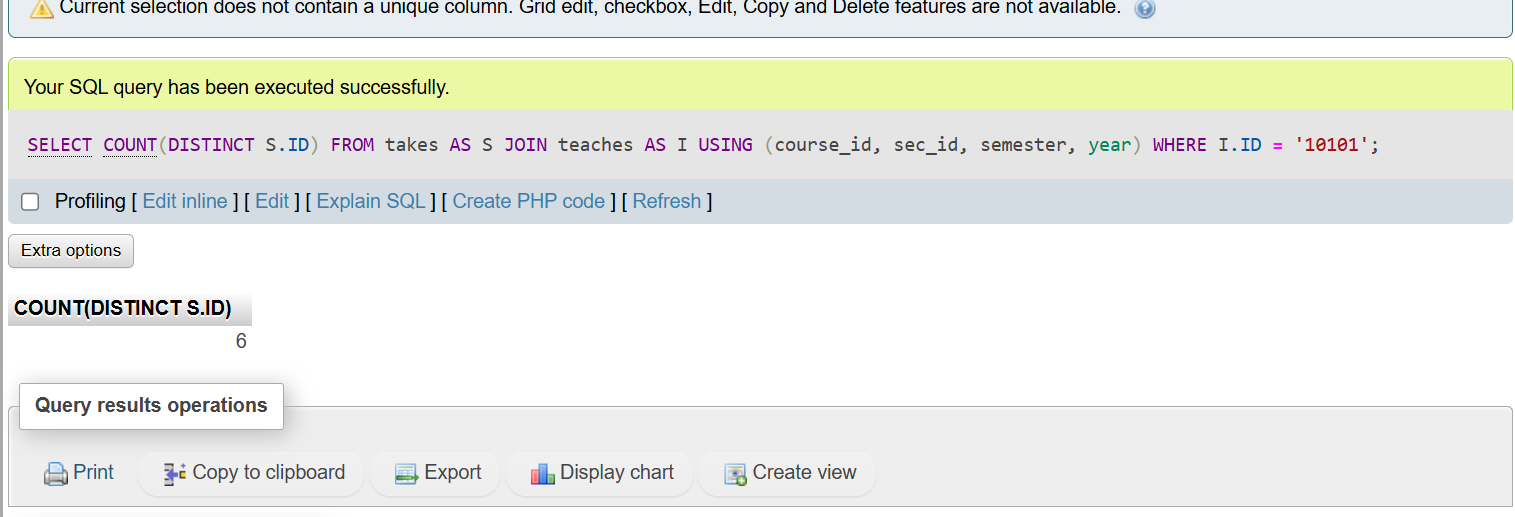
\includegraphics[width=1.0\textwidth]{fig/74.png}
    \caption{Query 74 Result}
\end{figure}

\begin{verbatim}
75. select count(distinct ID) from takes where (course_id, sec_id, semester, year) in (select course_id, sec_id, semester, year from teaches where teaches.ID=10101);
\end{verbatim}
\begin{figure}[h]
    \centering
    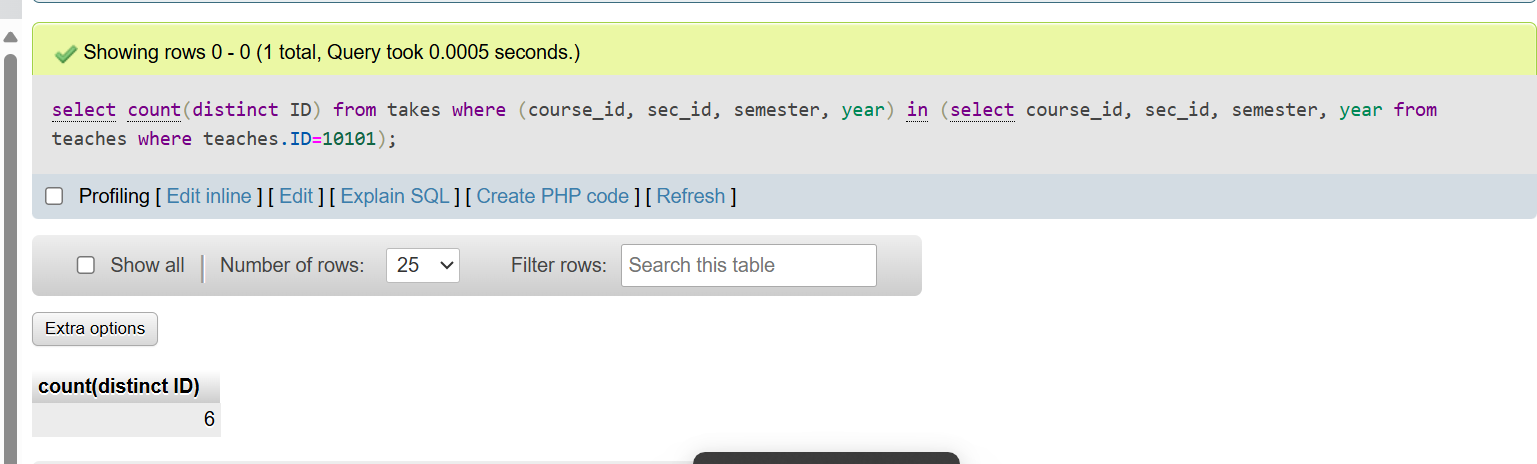
\includegraphics[width=1.0\textwidth]{fig/75.png}
    \caption{Query 75 Result}
\end{figure}

\begin{verbatim}
76. SELECT COUNT(DISTINCT ID) FROM takes WHERE (course_id, sec_id, semester, year) IN (SELECT course_id, sec_id, semester, year FROM teaches WHERE teaches.ID=10101);
\end{verbatim}
\begin{figure}[h]
    \centering
    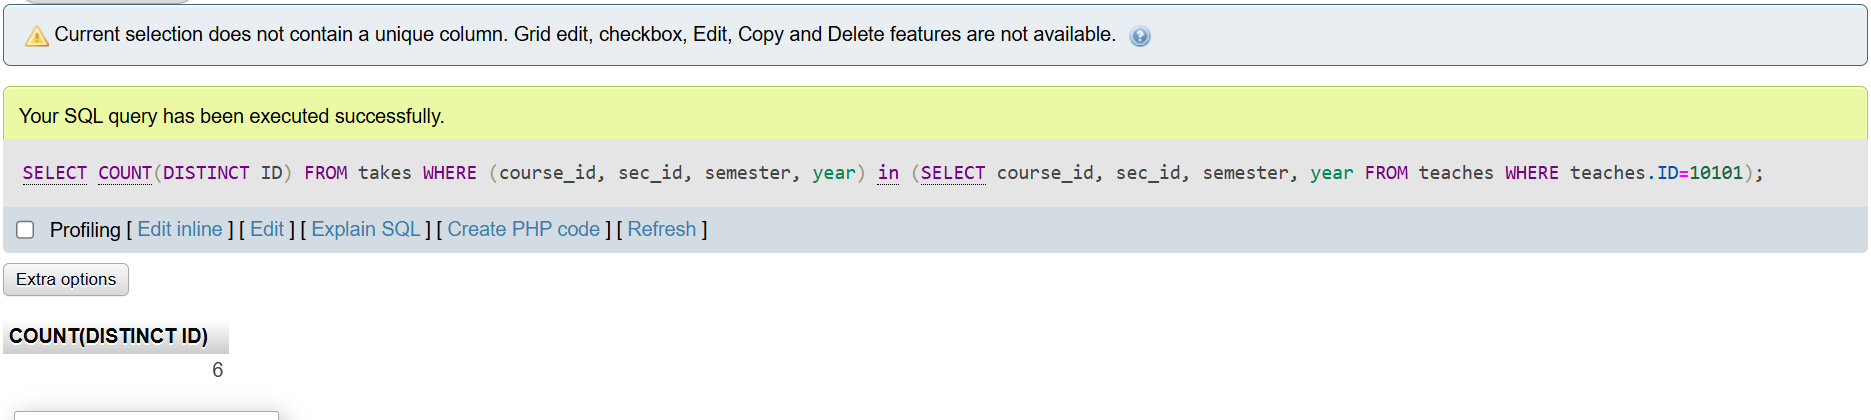
\includegraphics[width=1.0\textwidth]{fig/76.png}
    \caption{Query 76 Result}
\end{figure}

\begin{verbatim}
77. select DISTINCT T.name from instructor as T, instructor as S where T.salary > S.salary and S.dept_name='Biology';
\end{verbatim}
\begin{figure}[h]
    \centering
    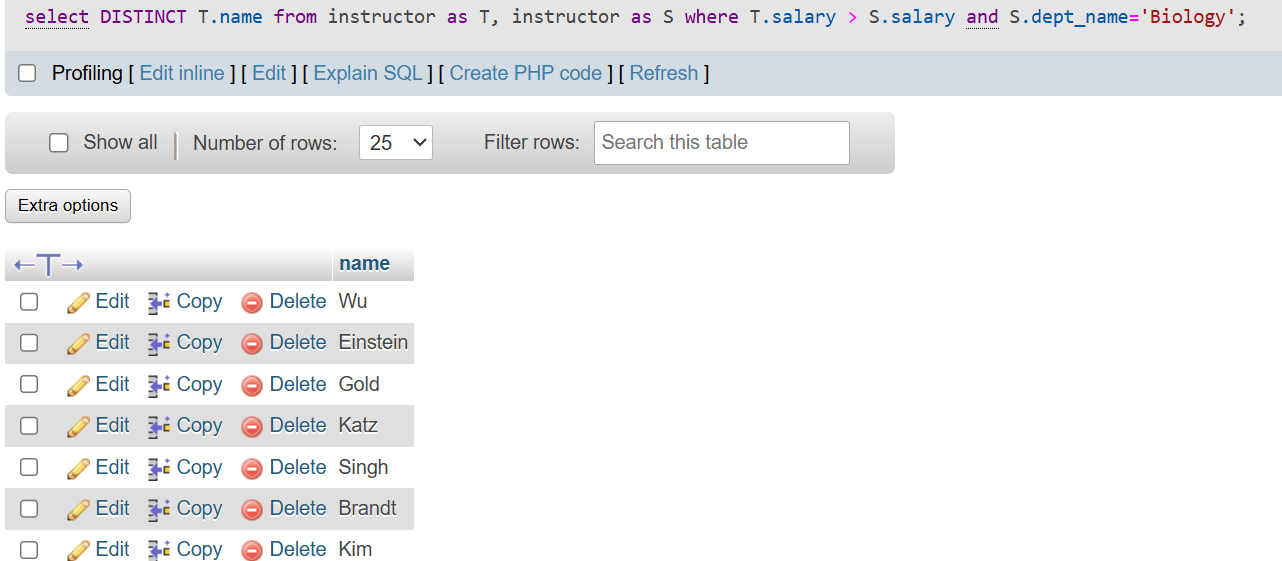
\includegraphics[width=1.0\textwidth]{fig/77.png}
    \caption{Query 77 Result}
\end{figure}

\begin{verbatim}
78. SELECT name FROM instructor WHERE salary > some (SELECT salary FROM instructor where dept_name='Biology');
\end{verbatim}
\begin{figure}[h]
    \centering
    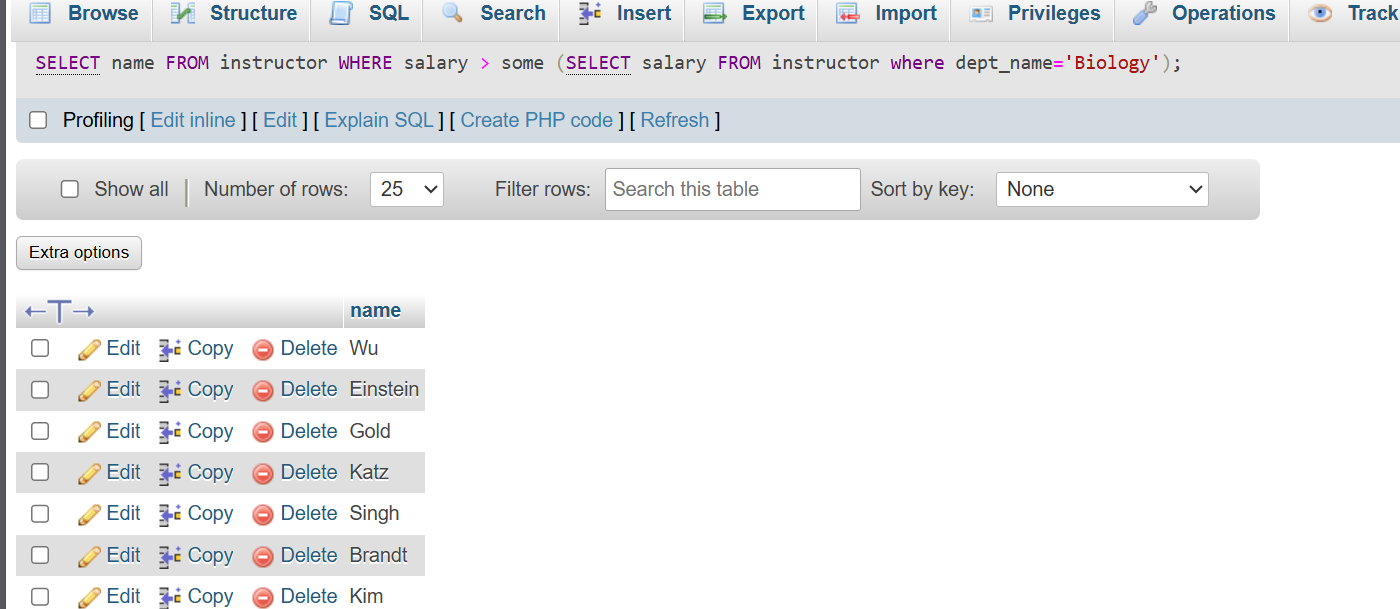
\includegraphics[width=1.0\textwidth]{fig/78.png}
    \caption{Query 78 Result}
\end{figure}

\begin{verbatim}
79. SELECT name FROM instructor WHERE salary > ALL (SELECT salary FROM instructor where dept_name='Biology');
\end{verbatim}
\begin{figure}[h]
    \centering
    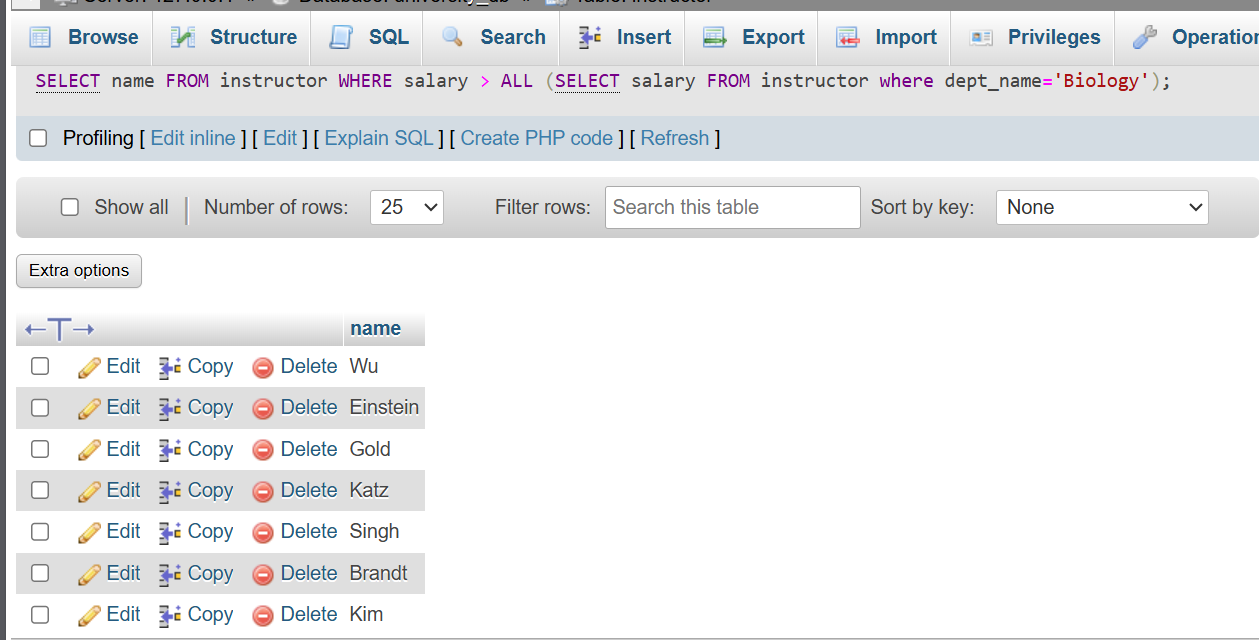
\includegraphics[width=1.0\textwidth]{fig/79.png}
    \caption{Query 79 Result}
\end{figure}

\begin{verbatim}
80. SELECT dept_name FROM instructor GROUP BY dept_name HAVING AVG (salary) >= ALL (SELECT AVG (salary) FROM instructor GROUP BY dept_name);
\end{verbatim}
\begin{figure}[h]
    \centering
    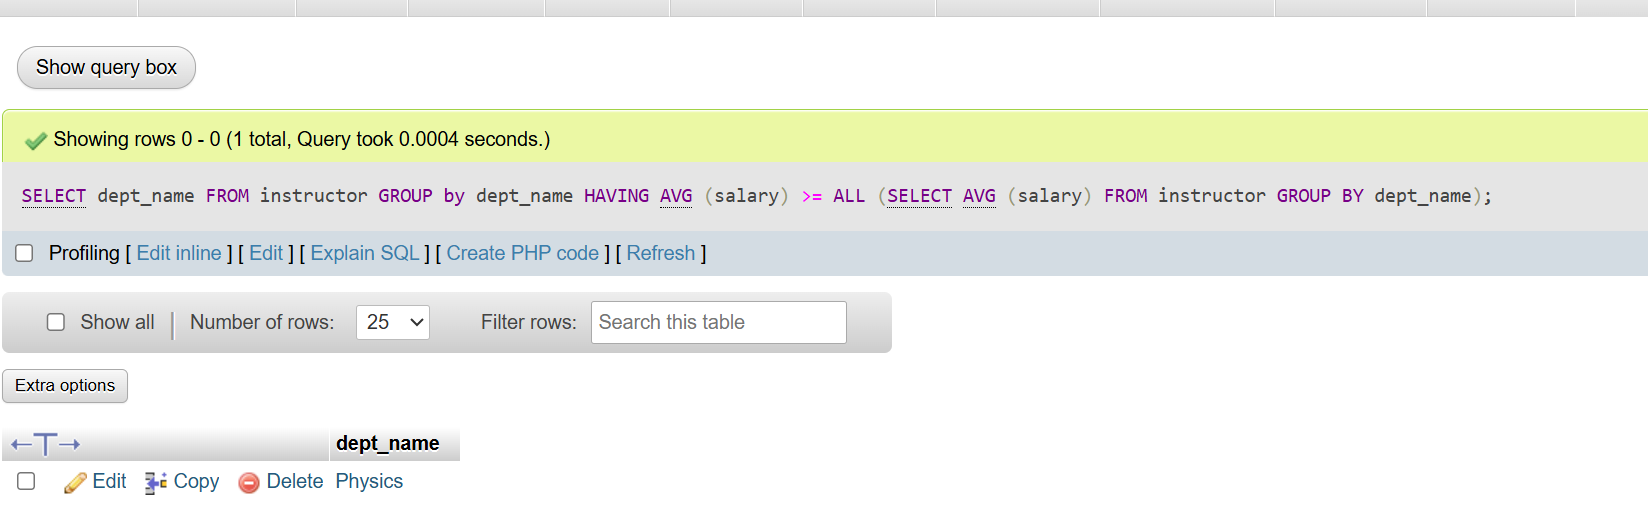
\includegraphics[width=1.0\textwidth]{fig/80.png}
    \caption{Query 80 Result}
\end{figure}

\begin{verbatim}
81. SELECT avg(salary) from instructor group by dept_name;
\end{verbatim}
\begin{figure}[h]
    \centering
    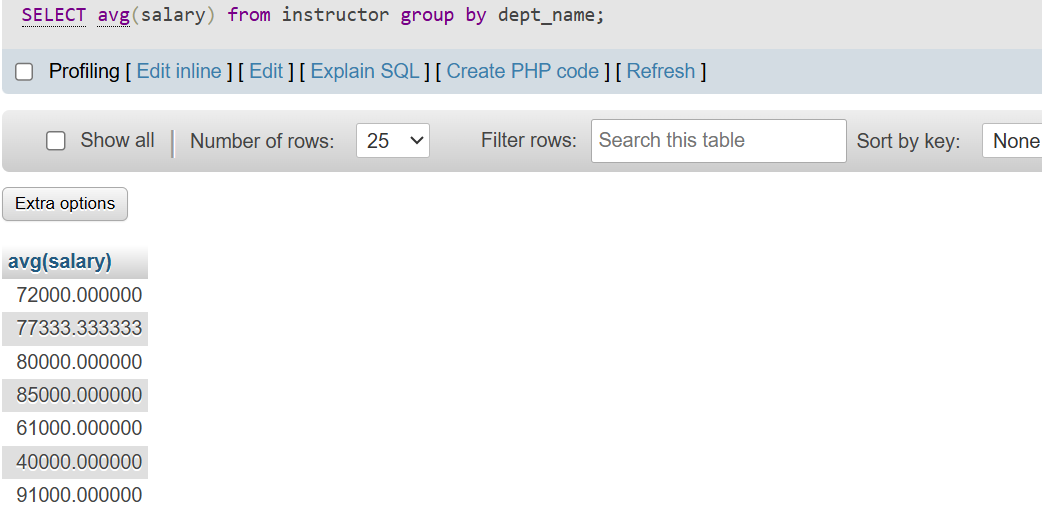
\includegraphics[width=1.0\textwidth]{fig/81.png}
    \caption{Query 81 Result}
\end{figure}

\begin{verbatim}
82. (select course_id from section where semester= 'Fall' and year='2009') intersect (select course_id from section where semester='Spring' and year='2010');
\end{verbatim}
\begin{figure}[h]
    \centering
    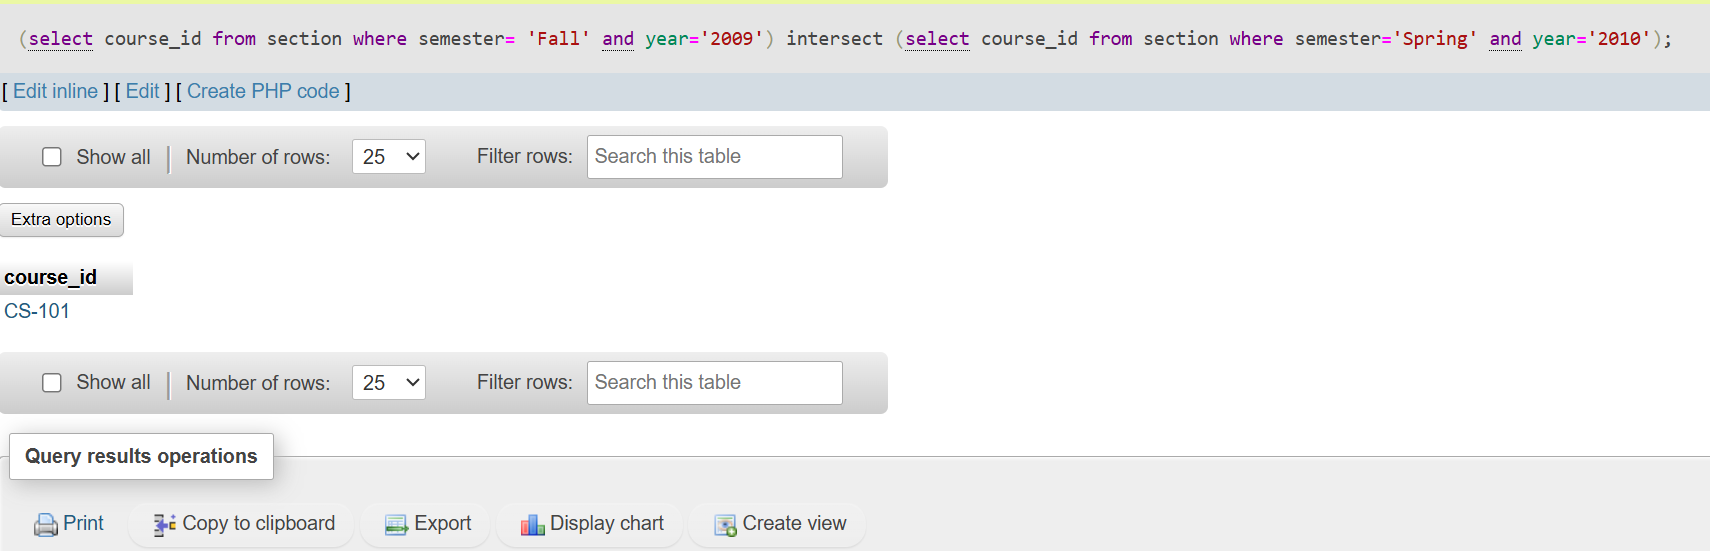
\includegraphics[width=1.0\textwidth]{fig/82.png}
    \caption{Query 82 Result}
\end{figure}

\begin{verbatim}
83. SELECT course_id 
FROM section AS S 
WHERE semester='Fall' AND year=2009 
AND EXISTS(
    SELECT * 
    FROM section AS T 
    WHERE semester='Spring' AND year=2010 
    AND S.course_id=T.course_id
);
\end{verbatim}
\begin{figure}[h]
    \centering
    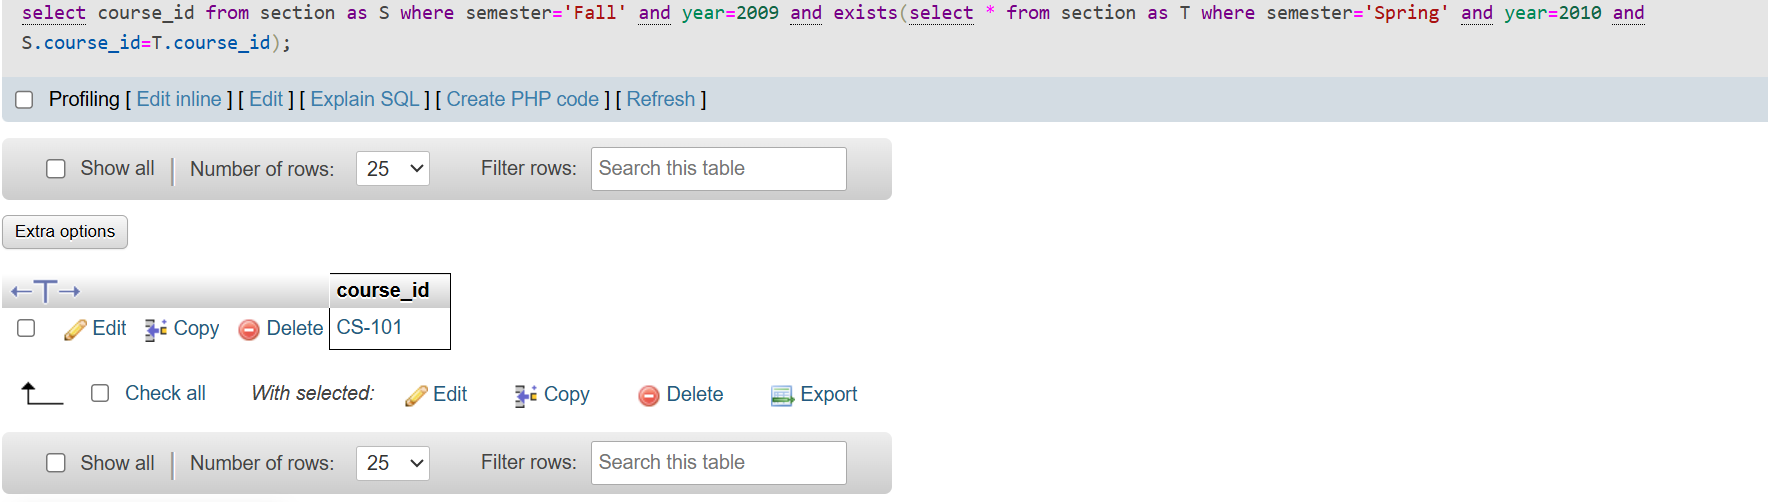
\includegraphics[width=1.0\textwidth]{fig/83.png}
    \caption{Query 83 Result}
\end{figure}

\begin{verbatim}
84. SELECT ID, name 
FROM student AS S 
WHERE NOT EXISTS(
    SELECT course_id 
    FROM course 
    WHERE dept_name='Biology'
) EXCEPT (
    SELECT T.course_id 
    FROM takes AS T 
    WHERE S.ID=T.ID
);
\end{verbatim}
\begin{figure}[h]
    \centering
    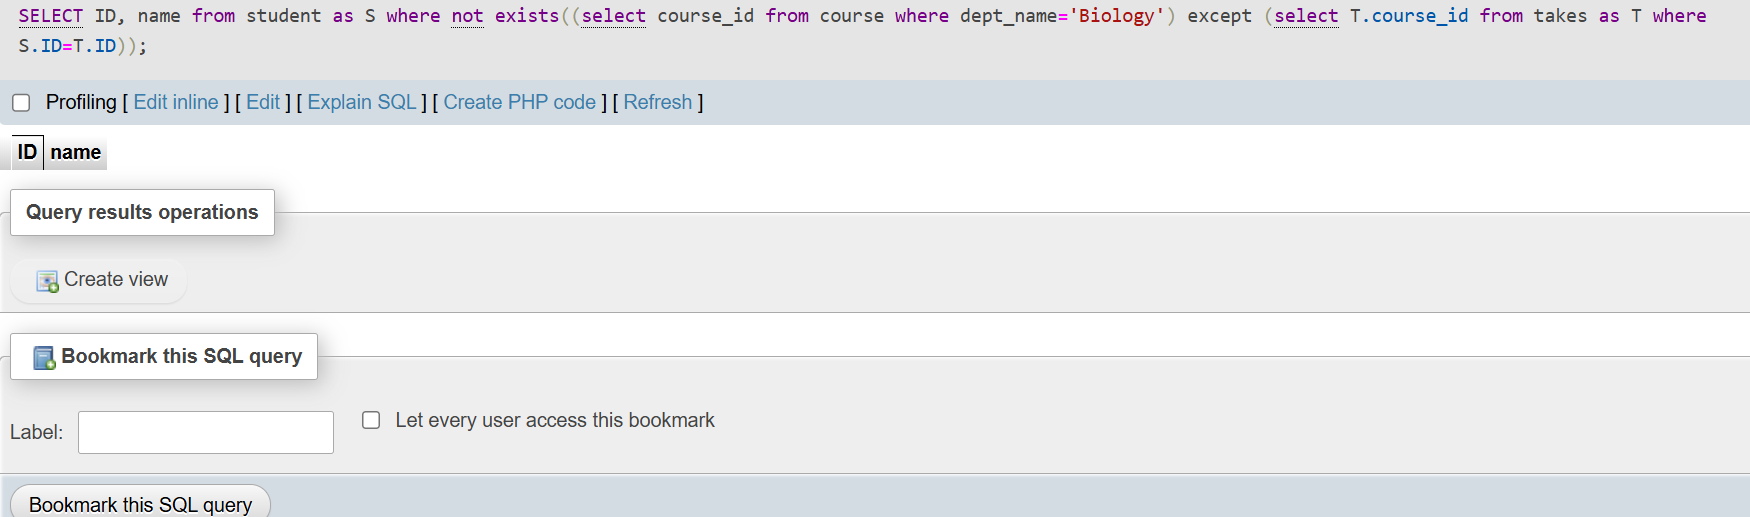
\includegraphics[width=1.0\textwidth]{fig/84.png}
    \caption{Query 84 Result}
\end{figure}

\begin{verbatim}
85. SELECT dept_name, AVG(salary) AS avg_salary 
FROM instructor 
GROUP BY dept_name 
HAVING avg_salary>42000;
\end{verbatim}
\begin{figure}[h]
    \centering
    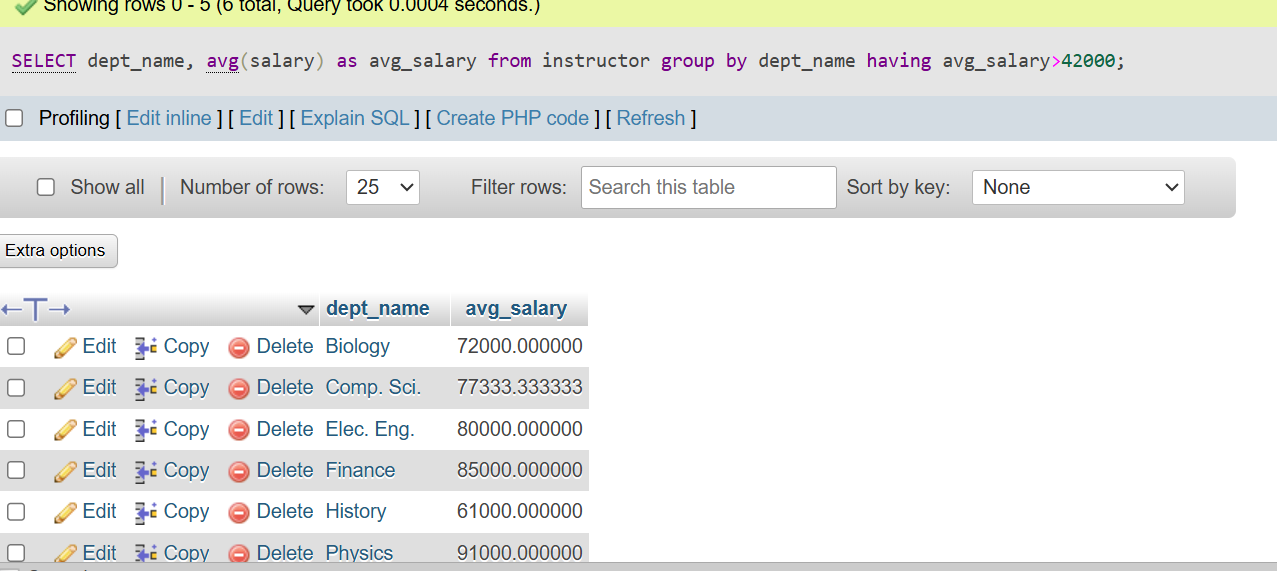
\includegraphics[width=1.0\textwidth]{fig/85.png}
    \caption{Query 85 Result}
\end{figure}

\begin{verbatim}
86. SELECT dept_name, avg_salary 
FROM (
    SELECT dept_name, AVG(salary) AS avg_salary 
    FROM instructor 
    GROUP BY dept_name
) AS subquery 
WHERE avg_salary>42000;
\end{verbatim}
\begin{figure}[h]
    \centering
    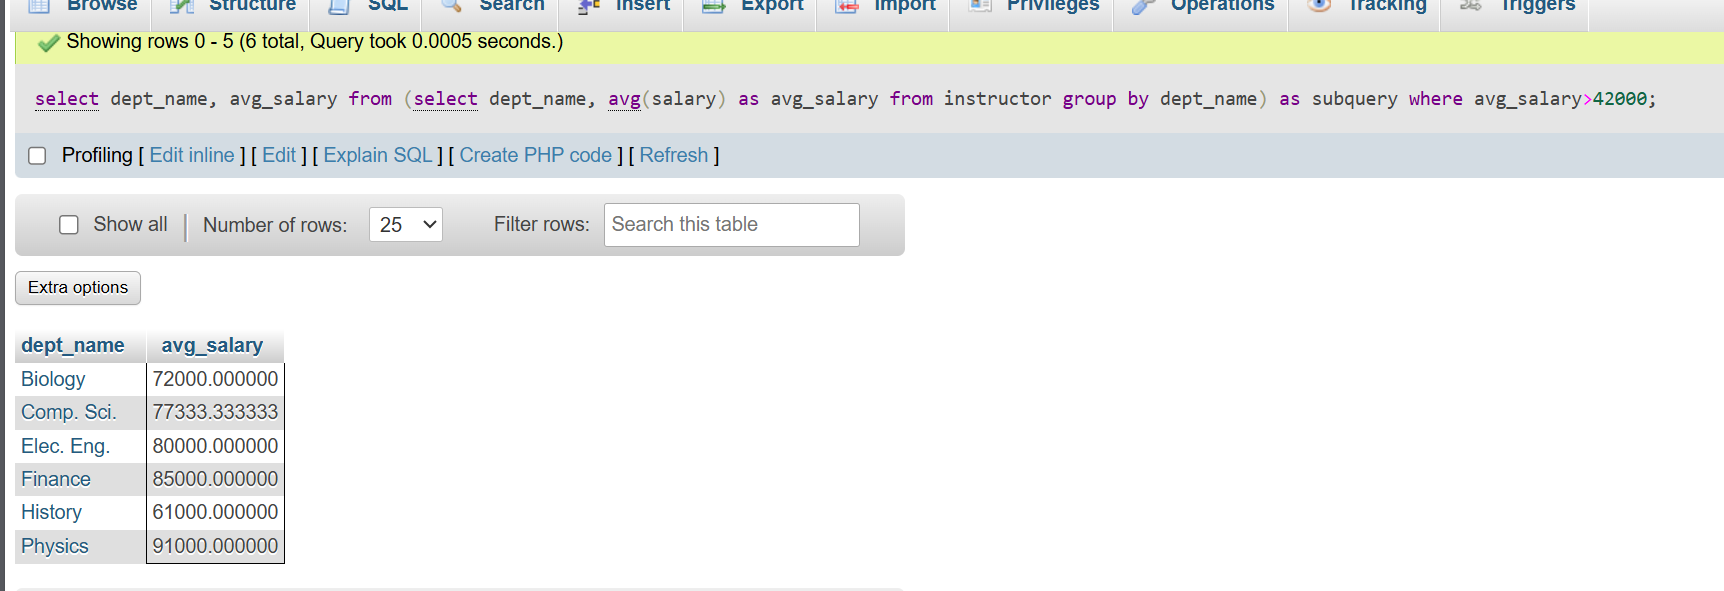
\includegraphics[width=1.0\textwidth]{fig/86.png}
    \caption{Query 86 Result}
\end{figure}

\begin{verbatim}
87. SELECT MAX(tot_salary) 
FROM (
    SELECT dept_name, SUM(salary) AS tot_salary 
    FROM instructor 
    GROUP BY dept_name
) AS subquery;
\end{verbatim}
\begin{figure}[h]
    \centering
    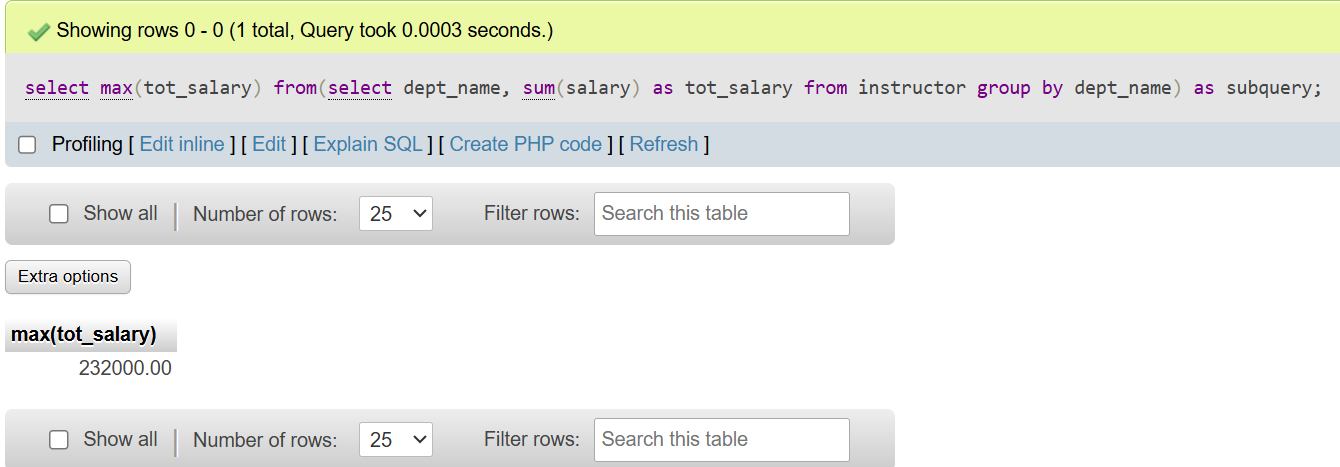
\includegraphics[width=1.0\textwidth]{fig/87.png}
    \caption{Query 87 Result}
\end{figure}

\begin{verbatim}
88. SELECT MAX(tot_salary) 
FROM (
    SELECT dept_name, SUM(salary) AS tot_salary 
    FROM instructor 
    GROUP BY dept_name
) AS dept_total;
\end{verbatim}
\begin{figure}[h]
    \centering
    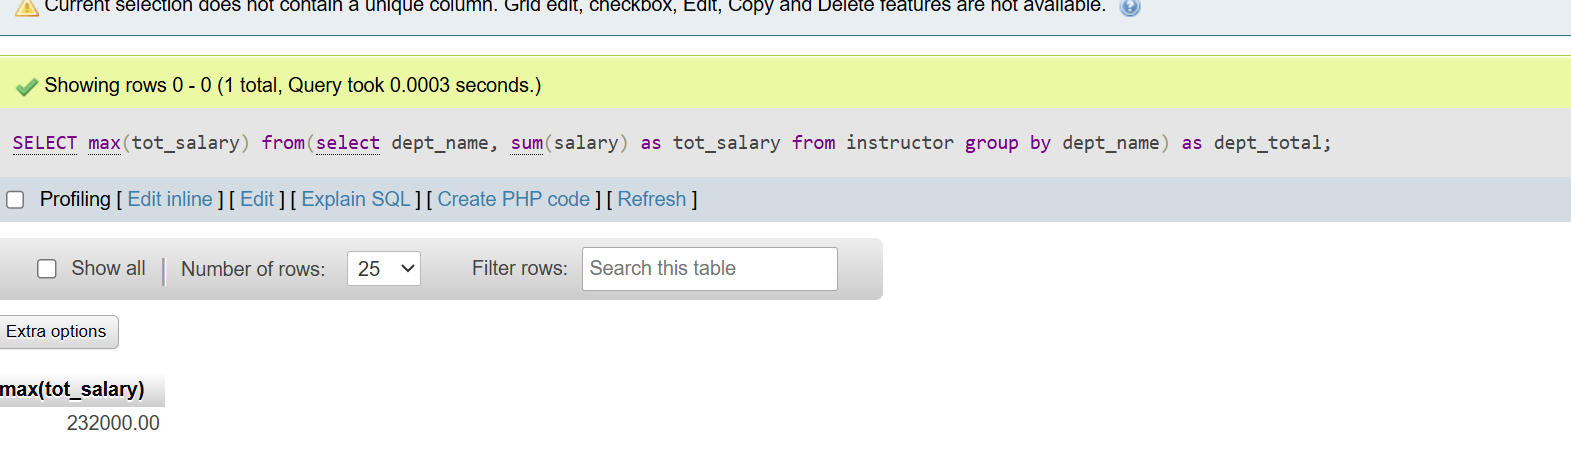
\includegraphics[width=1.0\textwidth]{fig/88.png}
    \caption{Query 88 Result}
\end{figure}

\begin{verbatim}
89. SELECT dept_name, (
    SELECT COUNT(*) 
    FROM instructor 
    WHERE department.dept_name = instructor.dept_name
) AS num_instructors 
FROM department;
\end{verbatim}
\begin{figure}[h]
    \centering
    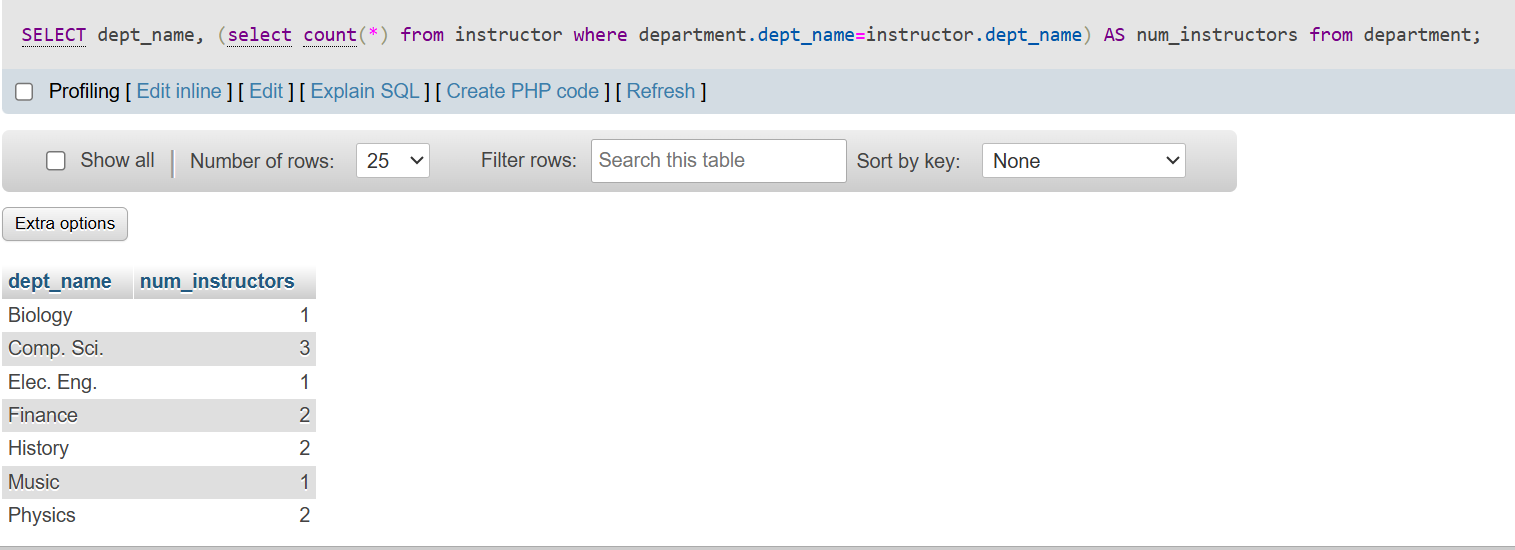
\includegraphics[width=1.0\textwidth]{fig/89.png}
    \caption{Query 89 Result}
\end{figure}
%%%%%%%%%%%%%%%%%%%%%%%%%%%%%%%%%%%%%%%%%%%%%%%%%%%%%%%%%%%%%%%%%%%%%%%%%%%%%%%%%%%%%%

\section{Second section}

%%%%%%%%%%%%%%%%%%%%%%%%%%%%%%%%%%%%%%%%%%%%%%%%%%%%%%%%%%%%%%%%%%%%%%%%%%%%%%%%%%%%%%%%%%%%
\begin{verbatim}
1. Find instructors with salary higher than their department's average
 and the difference.
SELECT instructor.ID, instructor.name, instructor.salary, 
       instructor.salary - dept_avg.avg_salary AS salary_difference,
       instructor.dept_name
FROM instructor
JOIN (
      SELECT dept_name, AVG(salary) AS avg_salary
      FROM instructor
      GROUP BY dept_name
     ) AS dept_avg ON instructor.dept_name = dept_avg.dept_name
WHERE instructor.salary > dept_avg.avg_salary
ORDER BY salary_difference DESC;
\end{verbatim}
\begin{figure}[h]
    \centering
    
\includegraphics[width=1.0\textwidth]{fig/task2/1.png}
    \caption{Query 1 Result}
\end{figure}

\begin{verbatim}
2. Courses taught in Fall 2009 and Spring 2010.
SELECT DISTINCT course.course_id, course.title
FROM course
JOIN section AS fall_section ON course.course_id = fall_section.course_id
JOIN section AS spring_section ON course.course_id = spring_section.course_id
WHERE fall_section.semester = 'Fall' 
  AND fall_section.year = 2009
  AND spring_section.semester = 'Spring' 
  AND spring_section.year = 2010;
\end{verbatim}
\begin{figure}[h]
    \centering
    
\includegraphics[width=1.0\textwidth]{fig/task2/2.png}
    \caption{Query 2 Result}
\end{figure}

\begin{verbatim}
3. Departments with total salary greater than budget.
SELECT department.dept_name, SUM(instructor.salary) AS total_salary, 
department.budget
FROM department
JOIN instructor ON department.dept_name = instructor.dept_name
GROUP BY department.dept_name, department.budget
HAVING SUM(instructor.salary) > department.budget;
\end{verbatim}
\begin{figure}[h]
    \centering
    
\includegraphics[width=1.0\textwidth]{fig/task2/3.png}
    \caption{Query 3 Result}
\end{figure}

\begin{verbatim}
4. Students who have taken courses from all departments.
SELECT student.ID, student.name
FROM student
WHERE NOT EXISTS (
    SELECT dept_name 
    FROM department
    EXCEPT
    SELECT DISTINCT course.dept_name
    FROM takes 
    JOIN course ON takes.course_id = course.course_id
    WHERE takes.ID = student.ID
);
\end{verbatim}
\begin{figure}[h]
    \centering
    
\includegraphics[width=1.0\textwidth]{fig/task2/4.png}
    \caption{Query 4 Result}
\end{figure}

\begin{verbatim}
5. Find the course with the highest number of students.
SELECT takes.course_id, course.title, COUNT(DISTINCT takes.ID) AS 
student_count
FROM takes
JOIN course ON takes.course_id = course.course_id
GROUP BY takes.course_id, course.title
HAVING COUNT(DISTINCT takes.ID) >= ALL (
    SELECT COUNT(DISTINCT ID)
    FROM takes
    GROUP BY course_id
);
\end{verbatim}
\begin{figure}[h]
    \centering
    
\includegraphics[width=1.0\textwidth]{fig/task2/5.png}
    \caption{Query 5 Result}
\end{figure}

\begin{verbatim}
6. Instructors who have never taught a course and their department's
 average salary.
SELECT instructor.ID, instructor.name, instructor.dept_name,
       AVG(dept_instructor.salary) AS dept_avg_salary
FROM instructor
LEFT JOIN teaches ON instructor.ID = teaches.ID
JOIN instructor AS dept_instructor ON instructor.dept_name = dept_instructor.dept_name
WHERE teaches.ID IS NULL
GROUP BY instructor.ID, instructor.name, instructor.dept_name;
\end{verbatim}
\begin{figure}[h]
    \centering
    
\includegraphics[width=1.0\textwidth]{fig/task2/6.png}
    \caption{Query 6 Result}
\end{figure}

\begin{verbatim}
7. Find students who have taken two courses in the same semester and year.
SELECT DISTINCT t1.ID, student.name, t1.semester, t1.year
FROM takes t1
JOIN takes t2 ON t1.ID = t2.ID 
              AND t1.course_id < t2.course_id
JOIN student ON t1.ID = student.ID
WHERE t1.semester = t2.semester 
  AND t1.year = t2.year;
\end{verbatim}
\begin{figure}[h]
    \centering
    
\includegraphics[width=1.0\textwidth]{fig/task2/7.png}
    \caption{Query 7 Result}
\end{figure}

\begin{verbatim}
8. Departments with the highest average student total credits and
instructor count.
SELECT student.dept_name, AVG(student.tot_cred) AS avg_credits,
       COUNT(DISTINCT instructor.ID) AS instructor_count
FROM student
LEFT JOIN instructor ON student.dept_name = instructor.dept_name
GROUP BY student.dept_name
HAVING AVG(student.tot_cred) >= ALL (
    SELECT AVG(tot_cred) 
    FROM student 
    GROUP BY dept_name
);
\end{verbatim}
\begin{figure}[h]
    \centering
    
\includegraphics[width=1.0\textwidth]{fig/task2/8.png}
    \caption{Query 8 Result}
\end{figure}

\begin{verbatim}
9. Courses that have never been taught and their department's 
total budget.
SELECT course.course_id, course.title, course.dept_name,
       department.budget AS dept_budget
FROM course
LEFT JOIN section ON course.course_id = section.course_id
JOIN department ON course.dept_name = department.dept_name
WHERE section.course_id IS NULL
ORDER BY department.budget DESC, course.course_id;
\end{verbatim}
\begin{figure}[h]
    \centering
    
\includegraphics[width=1.0\textwidth]{fig/task2/9.png}
    \caption{Query 9 Result}
\end{figure}

\begin{verbatim}
10. Find instructors who teach in every semester.
SELECT teaches.ID, instructor.name
FROM teaches
JOIN instructor ON teaches.ID = instructor.ID
GROUP BY teaches.ID, instructor.name
HAVING COUNT(DISTINCT semester) = (
    SELECT COUNT(DISTINCT semester) 
    FROM section
);
\end{verbatim}
\begin{figure}[h]
    \centering
    
\includegraphics[width=1.0\textwidth]{fig/task2/10.png}
    \caption{Query 10 Result}
\end{figure}

\begin{verbatim}
11. Students who have taken courses with all instructors in their 
department.
SELECT student.ID, student.name
FROM student
WHERE NOT EXISTS (
    SELECT instructor.ID
    FROM instructor
    WHERE instructor.dept_name = student.dept_name
    EXCEPT
    SELECT DISTINCT teaches.ID
    FROM takes 
    JOIN teaches ON takes.course_id = teaches.course_id
    WHERE takes.ID = student.ID
);
\end{verbatim}
\begin{figure}[h]
    \centering
    
\includegraphics[width=1.0\textwidth]{fig/task2/11.png}
    \caption{Query 11 Result}
\end{figure}

\begin{verbatim}
12. Find the building with the highest total classroom capacity and
 average room capacity.
SELECT classroom.building, 
       SUM(classroom.capacity) AS total_capacity,
       AVG(classroom.capacity) AS avg_capacity,
       COUNT(*) AS room_count
FROM classroom
GROUP BY classroom.building
HAVING SUM(classroom.capacity) >= ALL (
    SELECT SUM(capacity) 
    FROM classroom 
    GROUP BY building
);
\end{verbatim}
\begin{figure}[h]
    \centering
    
\includegraphics[width=1.0\textwidth]{fig/task2/12.png}
    \caption{Query 12 Result}
\end{figure}

\begin{verbatim}
13. Courses with more than 10 students and their average credits.
SELECT course.course_id, course.title, course.credits,
       COUNT(DISTINCT takes.ID) AS student_count
FROM course
JOIN takes ON course.course_id = takes.course_id
GROUP BY course.course_id, course.title, course.credits
HAVING COUNT(DISTINCT takes.ID) > 10
ORDER BY student_count DESC;
\end{verbatim}
\begin{figure}[h]
    \centering
    
\includegraphics[width=1.0\textwidth]{fig/task2/13.png}
    \caption{Query 13 Result}
\end{figure}

\begin{verbatim}
14. Find time slots with the most sections scheduled.
SELECT time_slot_id, COUNT(*) AS section_count
FROM section
GROUP BY time_slot_id
HAVING COUNT(*) >= ALL (
    SELECT COUNT(*)
    FROM section
    GROUP BY time_slot_id
);
\end{verbatim}
\begin{figure}[h]
    \centering
    
\includegraphics[width=1.0\textwidth]{fig/task2/14.png}
    \caption{Query 14 Result}
\end{figure}

\begin{verbatim}
15. Students who have taken every course in their department.
SELECT student.ID, student.name
FROM student
WHERE NOT EXISTS (
    SELECT course.course_id
    FROM course
    WHERE course.dept_name = student.dept_name
    EXCEPT
    SELECT takes.course_id
    FROM takes
    WHERE takes.ID = student.ID
);
\end{verbatim}
\begin{figure}[h]
    \centering
    
\includegraphics[width=1.0\textwidth]{fig/task2/15.png}
    \caption{Query 15 Result}
\end{figure}

\begin{verbatim}
16. Find the names of all students who have taken any 'Biology' 
course ever. With no duplicate names in the result.
SELECT DISTINCT name 
FROM student NATURAL JOIN takes NATURAL JOIN course 
WHERE dept_name = 'Biology';
\end{verbatim}
\begin{figure}[h]
    \centering
    
\includegraphics[width=1.0\textwidth]{fig/task2/16.png}
    \caption{Query 16 Result}
\end{figure}

\begin{verbatim}
17. Find the names of all instructors who have never taught a course.
SELECT name 
FROM instructor 
WHERE ID NOT IN (SELECT id FROM teaches);
\end{verbatim}
\begin{figure}[h]
    \centering
    
\includegraphics[width=1.0\textwidth]{fig/task2/17.png}
    \caption{Query 17 Result}
\end{figure}

\begin{verbatim}
18. For the student with ID 19991 and 98765, show all course_id 
and title of all courses registered for by the students.
SELECT course_id, title 
FROM course NATURAL JOIN takes 
WHERE ID IN (98765, 19991);
\end{verbatim}
\begin{figure}[h]
    \centering
    
\includegraphics[width=1.0\textwidth]{fig/task2/18.png}
    \caption{Query 18 Result}
\end{figure}

\begin{verbatim}
19. Find the names of courses in the Music department which have 3 credits.
SELECT title 
FROM course 
WHERE dept_name = 'Music' AND credits = 3;
\end{verbatim}
\begin{figure}[h]
    \centering
    
\includegraphics[width=1.0\textwidth]{fig/task2/19.png}
    \caption{Query 19 Result}
\end{figure}

\begin{verbatim}
20. Find the ID of the students that are taught by professor with ID 83821.
SELECT DISTINCT ID 
FROM takes 
WHERE (course_id, sec_id, semester, year) IN (
    SELECT course_id, sec_id, semester, year 
    FROM teaches 
    WHERE teaches.ID = 83821
); 
\end{verbatim}
\begin{figure}[h]
    \centering
    
\includegraphics[width=1.0\textwidth]{fig/task2/20.png}
    \caption{Query 20 Result}
\end{figure}
%%%%%%%%%%%%%%%%%%%%%%%%%%%%%%%%%%%%%%%%%%%%%%%%%%%%%%%%%%%%%%%%%%%%%%%%%%%%%%%%%%%%%%%%%%%%



\newpage

\endgroup
\end{document}
